%\documentclass[handout,ignorenonframetext,red]{beamer}
\documentclass[ignorenonframetext,red]{beamer}
%\documentclass[class=article, a4paper]{beamer}
%\documentclass[handout]{beamer} %pour sortie papier


\usepackage[french]{babel}
\usepackage{pgf,pgfarrows,pgfn odes,pgfautomata,pgfheaps,pgfs hade}
\usepackage{amsmath,amssymb}
\usepackage[utf8]{inputenc}
\usepackage{stmaryrd}
\usepackage{url}


%\documentclass[svgnames,ignorenonframetext]{beamer}
%\usepackage{times}
\usepackage{listings}
\usepackage{amsmath,multicol}
\usepackage{verbatim}
%\usepackage{beamerarticle}
\usepackage{longtable}
%\usepackage{ucs}
%\usepackage[utf8]{inputenc}
\usepackage{pdfpages}

\setcounter{tocdepth}{1}

\mode<presentation>
{
  \usetheme{Warsaw}
  \setbeamercovered{transparent}
  \AtBeginSection[]
  {
    \begin{frame}<beamer>
       \setcounter{tocdepth}{2}
       \tableofcontents[currentsection,currentsubsection,hideothersubsections]
    \end{frame}
  }

  \AtBeginSubsection[]
  {
    \begin{frame}<beamer>
    \frametitle{\thesection. \insertsectionhead}
       \tableofcontents[sectionstyle=hide/hide,subsectionstyle=show/shaded/hide ]
    \end{frame}
  }
  
  \addtobeamertemplate{footline}{\insertframenumber/\inserttotalframenumber}

}

%\mode<handout>{  \setbeamercolor{background canvas}{bg=black!5}} }


\logo{\vspace{-.10cm} \includegraphics[scale=0.1]{../illustration/logo_cnam.png}}
\date{\today}
\author{Rémi LEBLOND\\ \url{http://remileblond.fr/SMB137}}
\institute{Conservatoire National des Arts et Métiers - Centre de Strasbourg}



\title{SMB137 - Troisième partie}
\subtitle{Gestion des données}

\begin{document}
\frame[plain]{\titlepage}


\begin{frame}
 \frametitle{Plan}
 \tableofcontents
\end{frame} 

\section{Mémoire principale}

\subsection{Indexation des objets en mémoire}

\begin{frame}
 \frametitle{Von Neumann et mémoire principale}
2 idées de l’architecture Von Neumann :
\begin{itemize}
	\item Programme enregistré : 
	\begin{itemize}
	\item Toute instruction doit se trouver en mémoire pour pouvoir être exécutée
	\end{itemize}
	\item Mémoire adressable :
	\begin{itemize}
	\item L’unité centrale ne désigne jamais une valeur, mais l’adresse de la mémoire centrale dans laquelle celle-ci est stockée.
	\end{itemize}
\end{itemize}
 \end{frame}

\begin{frame}
\frametitle{Mémoire principale}
\begin{itemize}
\item <1> Mémoire à accès direct
\begin{itemize}
\item Structure de stockage directement adressable par le processeur
\item Seule structure externe au processeur accessible directement
\item Utilisation d'adresses mémoire
\end{itemize}

\item <2> Finalités de la mémoire principale :
\begin{itemize}
	\item Stockage d'informations (données / programmes)
	\item Indexation d'objets en mémoire
	\item Restitution d'informations
\end{itemize}

\end{itemize}
\end{frame}


\begin{frame}
\frametitle{Représentation de la mémoire}
\begin{itemize}
\item <1> Le bit : Unité d'information élémentaire (0 ou 1)
\item <2> Mémoire = tableau :
\begin{itemize}
\item chaque case mémorise un \textbf{bit} (chiffre binaire)
\item les bits sont regroupés en \textbf{cellules} (8, 12, 16, 32 ou 64 bits)
\item chaque cellule est identifiée par son \textbf{adresse}
\end{itemize}
\item <3> Capacité mémoire :
\begin{itemize}
\item quantité d’info pouvant y être stockées (en bits)
\item nombre de cellules pouvant être adressé
\end{itemize}
\end{itemize}
\end{frame}


\begin{frame}
\frametitle{Organisation de la mémoire principale}
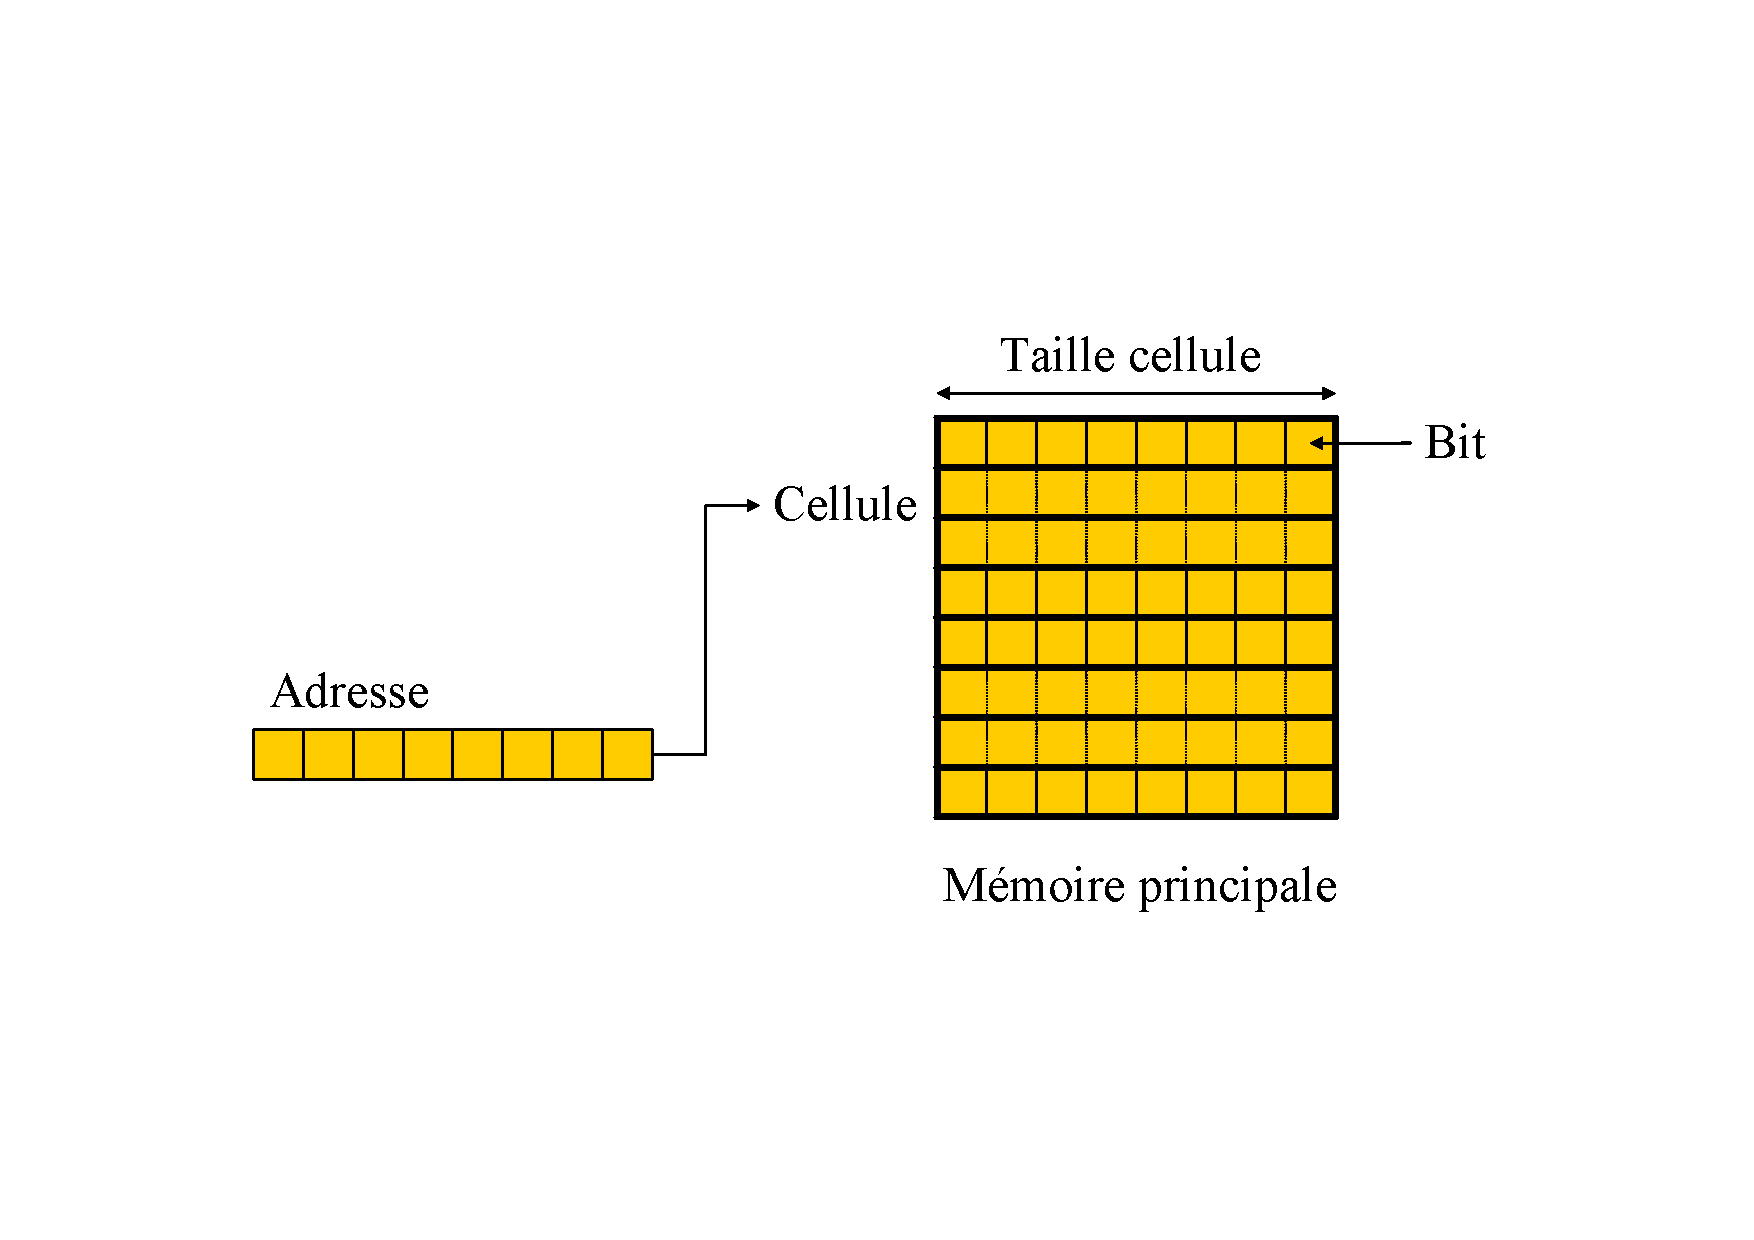
\includegraphics[width=\textwidth]{../illustration/memoire_principale_organisation.pdf}
\end{frame}

\begin{frame}
\frametitle{Adressage de la mémoire}
\begin{itemize}
\item Cellule : plus petite unité adressable
\item Adresse sur k bits $\rightarrow$ adressage de $2^k$ mots mémoire
\end{itemize}

\begin{block}{Correspondances pratiques}
\begin{tabular}{c|r}
Taille de l'adresse & Nombre de mots adressables \\
\hline
8 bits & 256 \\
16 bits & 65 536 \\
32 bits & 4 294 967 296 \\
64 bits & 18 446 744 073 709 600 000 \\
\end{tabular}
\end{block}
\end{frame}



\begin{frame}
\frametitle{Exemples de structures de stockage pour 96 bits}
12 cellules de 8 bits / 8 cellules de 12 bits / 6 cellules de 16 bits

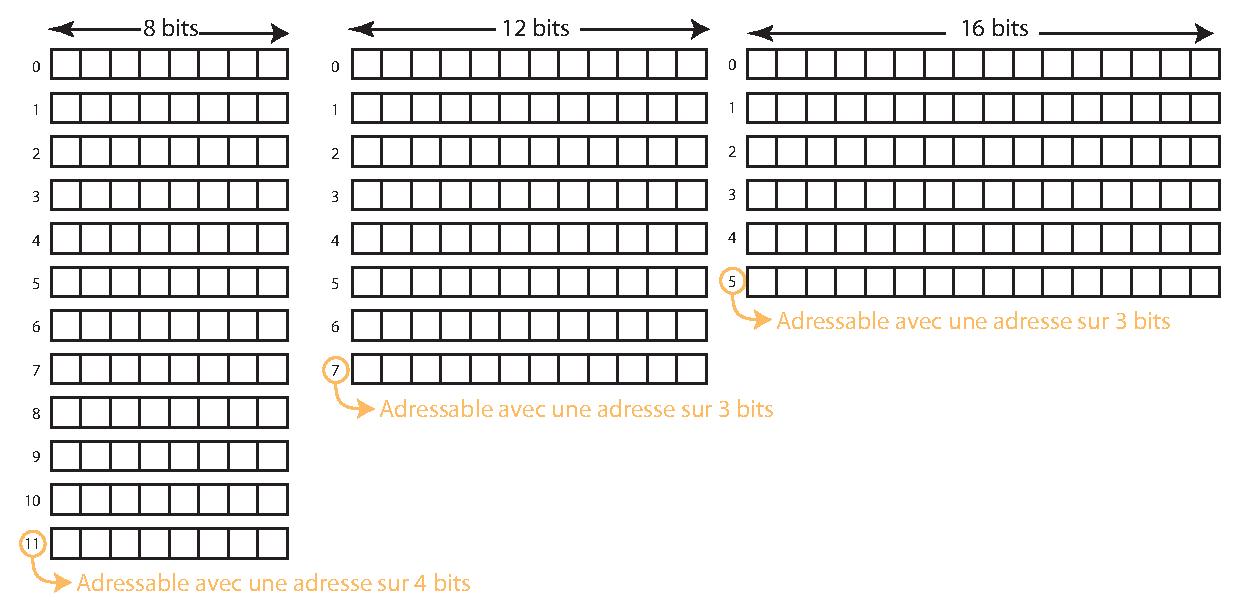
\includegraphics[width=\textwidth]{../illustration/stockage96bits.pdf}
\end{frame}

\begin{frame}
\frametitle{Exemples de tailles de cellules}
\begin{table}[htdp]
\begin{center}
\begin{tabular}{|c|c|}
\hline
Ordinateur & Bits par cellule \\
\hline
Burrought B1700 & 1 \\
IBM PC & \textbf{8} \\
DEC PDP-8 & 12 \\
DEC PDP-15 & 18 \\
XDS Sigma 9 & 32 \\
CDC Cyber & 60 \\
\hline
\end{tabular}
\end{center}
\label{default}
\end{table}
Aujourd'hui, l'utilisation de cellules de 8 bits (un octet) est devenu la norme
\end{frame}

\begin{frame}
 \frametitle{Burrought B1700}
 \begin{figure}[htbp]
\begin{center}
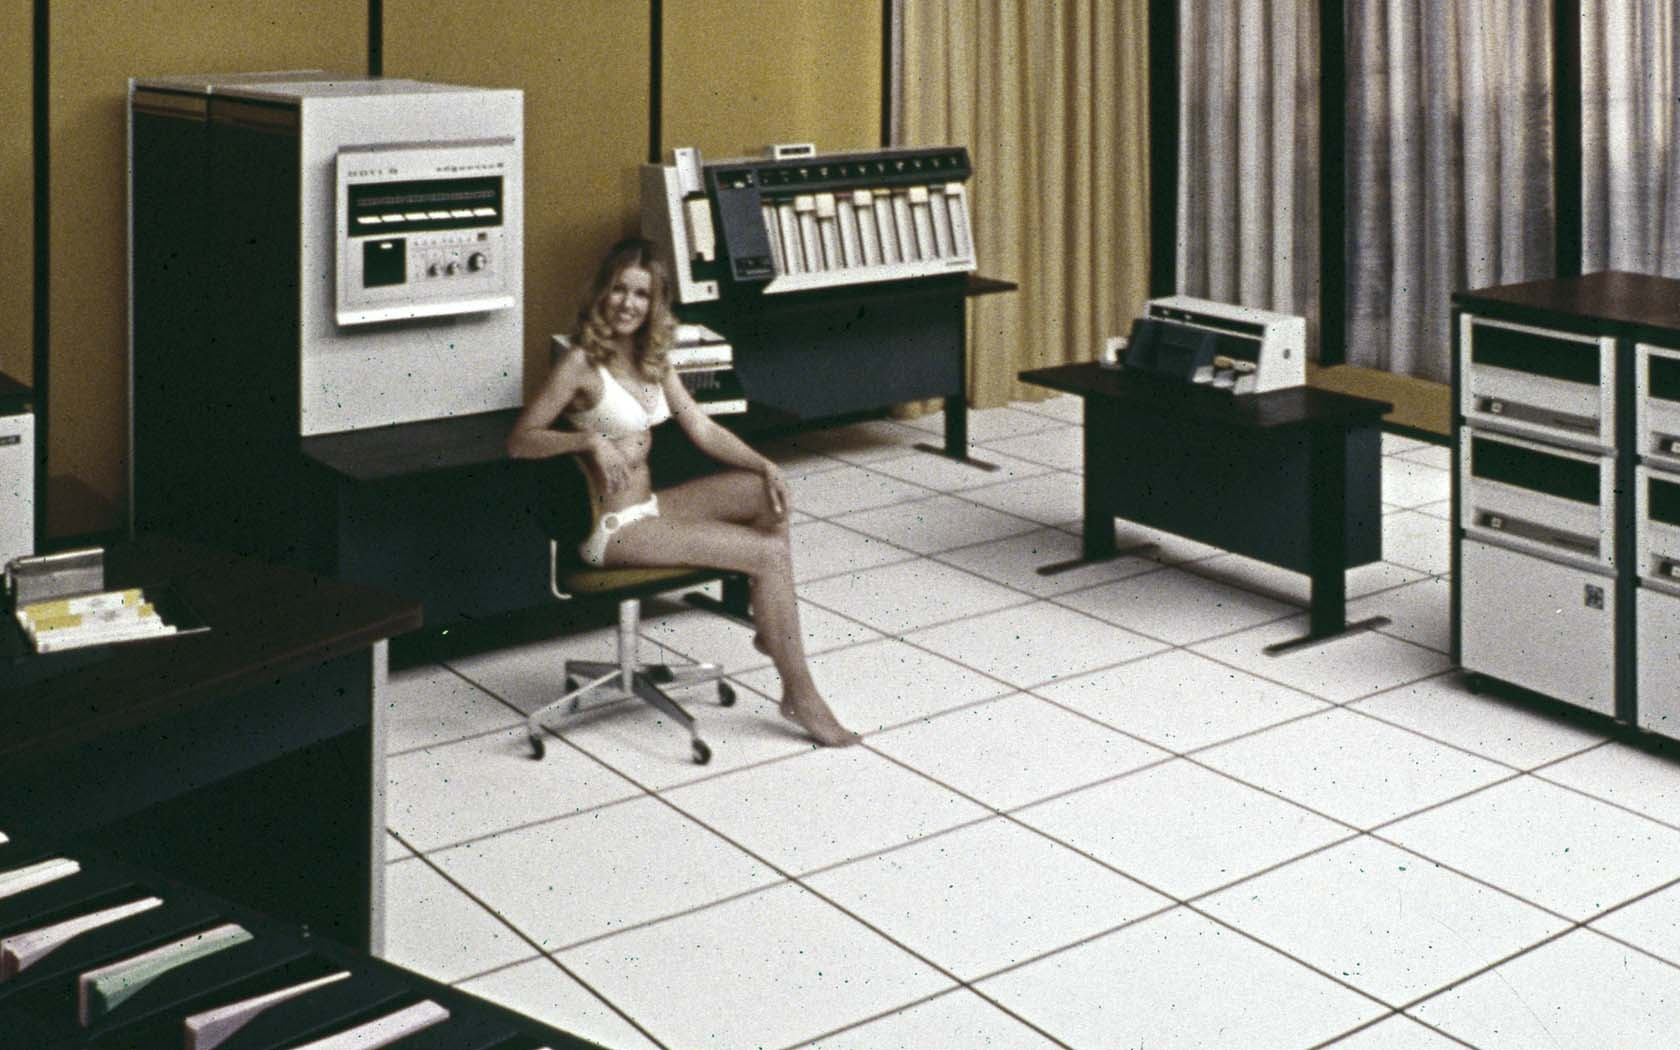
\includegraphics[width=.9\textwidth]{../illustration/BurroughtB1700.jpg}
\caption{Photo publicitaire du Burroughs B1700 (1972)\cite{B1700}}
\label{default}
\end{center}
\end{figure}
\end{frame}

\begin{frame}
\frametitle{Regroupement des octets en mots}
Avec des cellules de 8 bits (un octet) :
\begin{itemize}
\item Chaque cellule contient un octet
\item Les octets sont regroupés en mots
\begin{itemize}
\item machines 32 bits $\rightarrow$ mots de 4 octets
\item machines 64 bits $\rightarrow$ mots de 8 octets
\end{itemize}
\item La plupart des instructions manipule des mots entiers (addition, par exemple)
\end{itemize}
\end{frame}


\begin{frame}
\frametitle{Ordonnancement des octets}
Au sein d'un mot, les octets sont numérotés :
\begin{itemize}
\item <1> \textbf{Big endian} : de gauche à droite $\longmapsto$
\begin{itemize}
\item gros-boutiste\footnote{"Les voyages de Gulliver", de Jonathan Swift.}
\item octet de poids fort en tête
\end{itemize}
\small{\textit{Exemples : Sparc, Motorola 68000, Mainframe IBM, JVM, IP...}}

\item <2> \textbf{Little endian} : de droite à gauche $\longmapsfrom$
\begin{itemize}
\item petit-boutisme
\item octet de poids faible en tête
\end{itemize}
\small{\textit{Exemple : Intel}}
\end{itemize}
\end{frame}

\begin{frame}
\frametitle{Ordonnancement des octets}
\begin{exampleblock}{Ex. : 192.168.0.1}
\begin{itemize}
\item Big endian : octet de poids fort à gauche 

192.168.0.1
\item Little endian : octet de poids fort à droite

1.0.168.192
\end{itemize}
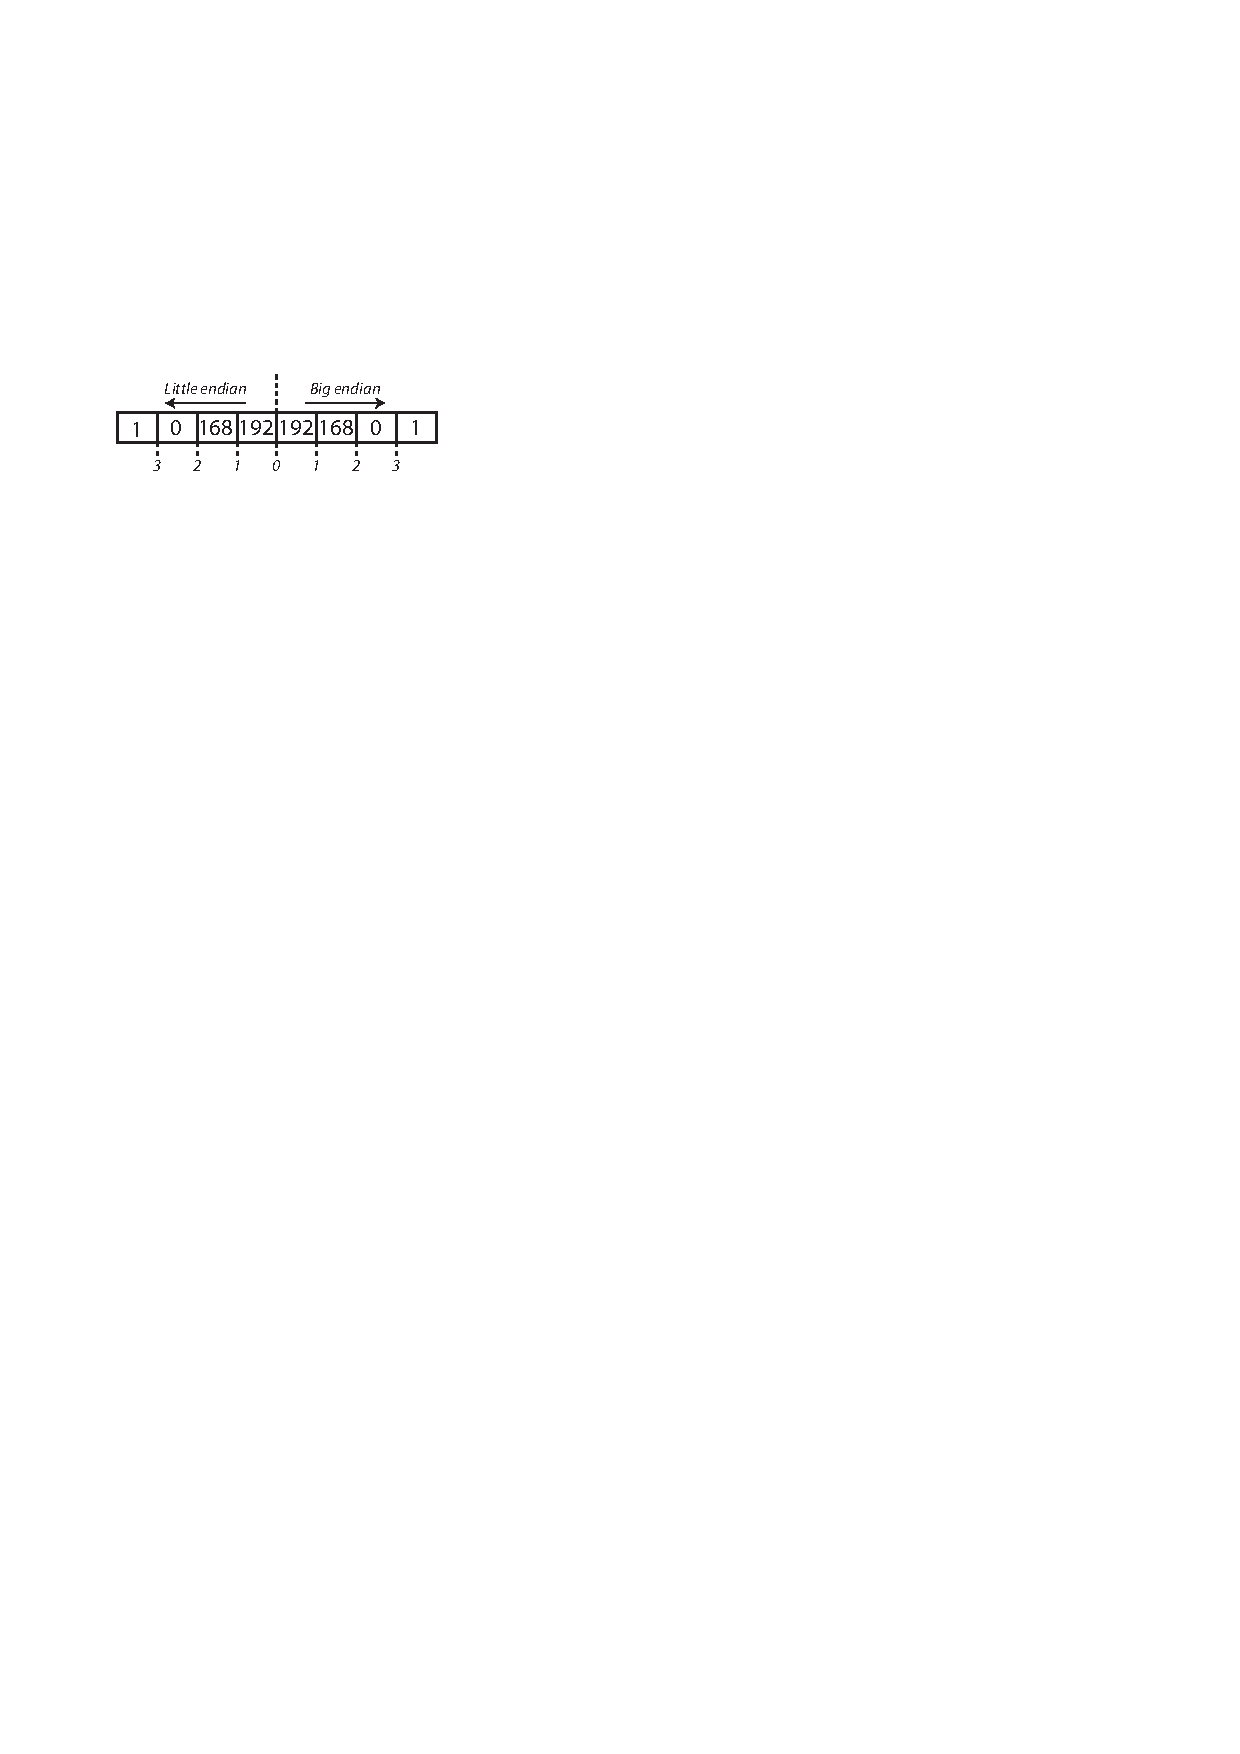
\includegraphics[width=\textwidth]{../illustration/little_big_endian.pdf}
\end{exampleblock}
\end{frame}


\begin{frame}
\frametitle{Ordonnancement des octets}
\textbf{Bi-endian}, bytesexual ou biboutiste
\begin{itemize}
\item choix de l'octet de poids fort par logiciel et/ou matériel
\end{itemize}

\begin{exampleblock}{Exemples}
\begin{itemize}
\item PowerPC (IBM)
\item ARM
\item DEC Alpha
\item MIPS
\item PA-RISC (HP)
\item IA-64 (Intel)
\end{itemize}

\end{exampleblock}
\end{frame}

\begin{frame}
\frametitle{Ordonnancement des octets}
Problème de compatibilité :
\begin{itemize}
\item dès que les échanges portent sur plus d'un octet
\begin{itemize}
\item incompatibilité binaire
\end{itemize}
\item échange via un réseau
\begin{itemize}
\item protocole IP : big endian
\end{itemize}

\item conversions complexes et coûteuses
\end{itemize}
\end{frame}

\begin{frame}
\frametitle{Codes correcteurs d'erreurs}
\begin{itemize}
\item <1> Codes détecteurs/correcteurs d'erreurs
\begin{itemize}
\item bits supplémentaires (redondance)
\item protocole de validation
\item vérification systèmatique et interruption en cas d'erreur
\end{itemize}
\item <2> Distance de Hamming\footnote{Richard HAMMING, 1950} :
\begin{itemize}
\item comparaison de mots binaires par OU exclusif
\item exemple : \texttt{11100101} et \texttt{00100100} sont distants de 3 bits
\item qualification des algorithmes : 
\begin{itemize}
\item 1 bit de parité $\rightarrow$ DH2
\end{itemize}
\end{itemize}
\end{itemize}
\end{frame}

\begin{frame}
\frametitle{Algorithme de détection/correction de Hamming}
Regroupement des données par zones
\begin{itemize}
\item Ajout d'un bit de parité dans chaque zone
\item Calcul de la parité de chaque zone
\item Détection et correction d'erreur
\end{itemize}
\begin{exampleblock}{Exemple : Stockage de la chaîne \texttt{0111}}
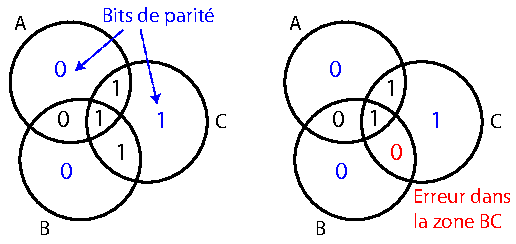
\includegraphics{../illustration/hamming.pdf}
\end{exampleblock}
\end{frame}

\begin{frame}
\frametitle{Algorithme de détection/correction de Hamming}
\begin{itemize}
\item Cas pratique \cite{tanen} :
\begin{itemize}
\item prise en charge d'un mot de 16 bits : \texttt{1111000010101110}
\item ajout de 5 bits de parité (1, 2, 4, 8 et 16)
\item $\rightarrow$ stockage sur 21 bits
\end{itemize}
\item Correspondance du contrôle de parité :
\begin{itemize}
\item bit 5 $\rightarrow$ 4 et 1 ($4+1=5$)
\item bit 6 $\rightarrow$ 4 et 2 ($4+2=6$)
\end{itemize}
\end{itemize}

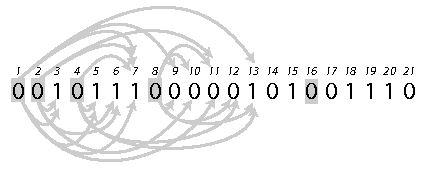
\includegraphics{../illustration/hamming_exemple.pdf}
\end{frame}


\begin{frame}
\frametitle{Représentation des adresses mémoire}
\begin{itemize}
\item Code source :
\begin{itemize}
\item Adresses symboliques
\begin{itemize}
\item Variable "compteur"
\end{itemize}
\end{itemize}
\item <2->Module objet :
\begin{itemize}
\item Adresses translatables
\begin{itemize}
\item "50$^{eme}$ mot depuis le début espace de l'espace d'adressable du module"
\end{itemize}
\end{itemize}
\item <3->Liaison, chargement :
\begin{itemize}
\item Adresses absolues
\begin{itemize}
\item Emplacement mémoire situé à l’adresse "xxxx"
\end{itemize}
\end{itemize}
\end{itemize}
\end{frame}


\begin{frame}
\frametitle{Liaison d’adresses}
\begin{itemize}
\item Programme réside sur disque 
\begin{itemize}
\item Fichier exécutable $\rightarrow$ adressage logique
\end{itemize}
\item Chargé en mémoire pour être exécuté
\begin{itemize}
\item Emplacements mémoire $\rightarrow$ adressage physique
\end{itemize}
\item Peut résider dans une partie quelconque de la mémoire
\begin{itemize}
\item Programmes translatables
\item Exceptions : 
\begin{itemize}
\item \texttt{.com} de MS/DOS (compilation statique)
\item Chargement paramètré (\texttt{himem.sys})
\end{itemize}
\end{itemize}
\end{itemize}
\end{frame}

\begin{frame}
\frametitle{Adressage logique ou physique}
\begin{itemize}
\item <1>L’unité centrale manipule des \textbf{adresses logiques} (emplacement relatif à l'espace d'adressage)
\begin{itemize}
\item Les programmes ne connaissent que des adresses logiques, ou virtuelles
\end{itemize}
\item <2>L’unité mémoire manipule des \textbf{adresses physiques} (emplacement physique de la mémoire)
\begin{itemize}
\item Les adresses physiques ne sont jamais vues par les programmes utilisateurs
\item Ils ne peuvent pas connaître l'emplacement mémoire physique 
\end{itemize}
\end{itemize}
\end{frame}


\begin{frame}
\frametitle{Adressage logique ou physique}
Pour un processus :
\begin{itemize}
\item Espace d’adressage logique (virtuel) :
\begin{itemize}
\item Ensemble des adresses pouvant être générées par un programme
\end{itemize}
\item Espace d’adressage physique :
\begin{itemize}
\item Ensemble des adresses physiques correspondant à l'ensemble des adresses logiques
\end{itemize}
\end{itemize}
\end{frame}


\begin{frame}
\frametitle{La gestion de la mémoire}
La gestion de la mémoire a trois objets :
\begin{itemize}
\item <1> \textbf{Traduire} les adresses logiques $\rightarrow$ adresses physiques
\begin{itemize}
\item Mise en place des paramètres de calcul d'adresse permettant la translation des adresses
\item Traduction à la volée
\end{itemize}

\item <2> \textbf{Protéger} la mémoire allouée aux différents processus

\item <3> \textbf{Partager}  la mémoire entre les différents processus du système
\begin{itemize}
\item Ressource sensible et toujours limitée
\end{itemize}

\end{itemize}
\end{frame}

\begin{frame}
\frametitle{Virtualisation des adresses mémoire}
\begin{itemize}
\item <1>Exécution du programme sans modification
\begin{itemize}
\item Chargement tel quel à partir du fichier
\item Sans traduction des adresses
\end{itemize}

\item <2>Permet de faire abstraction de l’emplacement physique du processus en mémoire physique
\item <3>La virtualisation de l’accès à la mémoire permet :
\begin{itemize}
\item d’écrire des programmes portables
\begin{itemize}
\item indépendants de l’architecture physique
\end{itemize}

\item d'utiliser un même programme dans plusieurs processus différents
\end{itemize}
\end{itemize}
\end{frame}

\begin{frame}
\frametitle{Fonction de calcul d’adresse}
\begin{itemize}
\item <1>Réalisée lors du décodage de l’instruction courante
\begin{itemize}
\item Fournit l’adresse logique de l’objet recherché en mémoire
\item Traduction adresse logique $\rightarrow$ adresse physique
\item La CPU ne désigne jamais une valeur, mais son index de classement dans l’espace d’adressage logique
\end{itemize}
\item <2>Impossible sans l'aide du matériel
\begin{itemize}
\item Protection mémoire
\item Unité de gestion de la mémoire
\end{itemize}
\end{itemize}
\end{frame}


\begin{frame}
\frametitle{Fonction de calcul d'adresse}
\begin{itemize}
\item Ne doit pas ralentir les accès à la mémoire
\item Transformation adresse virtuelle $\rightarrow$ adresse physique : matériel
\item Lors de l'exécution des instructions (runtime)
\end{itemize}
\end{frame}



%-----------------------------------------------
\subsection{Mémoire linéaire}
%-----------------------------------------------


\begin{frame}
\frametitle{Cas des machines mono-programmées}
\begin{itemize}
\item Un seul utilisateur possible
\begin{itemize}
\item Totale disponibilité de la mémoire pour l'utilisateur
\end{itemize}
\item Pas de matériel spécifique pour la gestion de la mémoire
\begin{itemize}
\item Impossible de protéger le programme contre les débordements des autres
\end{itemize}
\item Cohabitation de programmes difficile
\end{itemize}
\end{frame}


\begin{frame}
\frametitle{Cas des machines mono-programmées}
\begin{itemize}
\item Solution simple et rapide en exécution
\item Solution retenue par :
\begin{itemize}
\item Les premiers systèmes à traitement par lot
\item Les premiers ordinateurs personnel
\end{itemize}
\item Taille maximale d'un programme limitée par la taille mémoire (découpage overlay)
\end{itemize}
\end{frame}


\begin{frame}
\frametitle{Machine mono programmée}
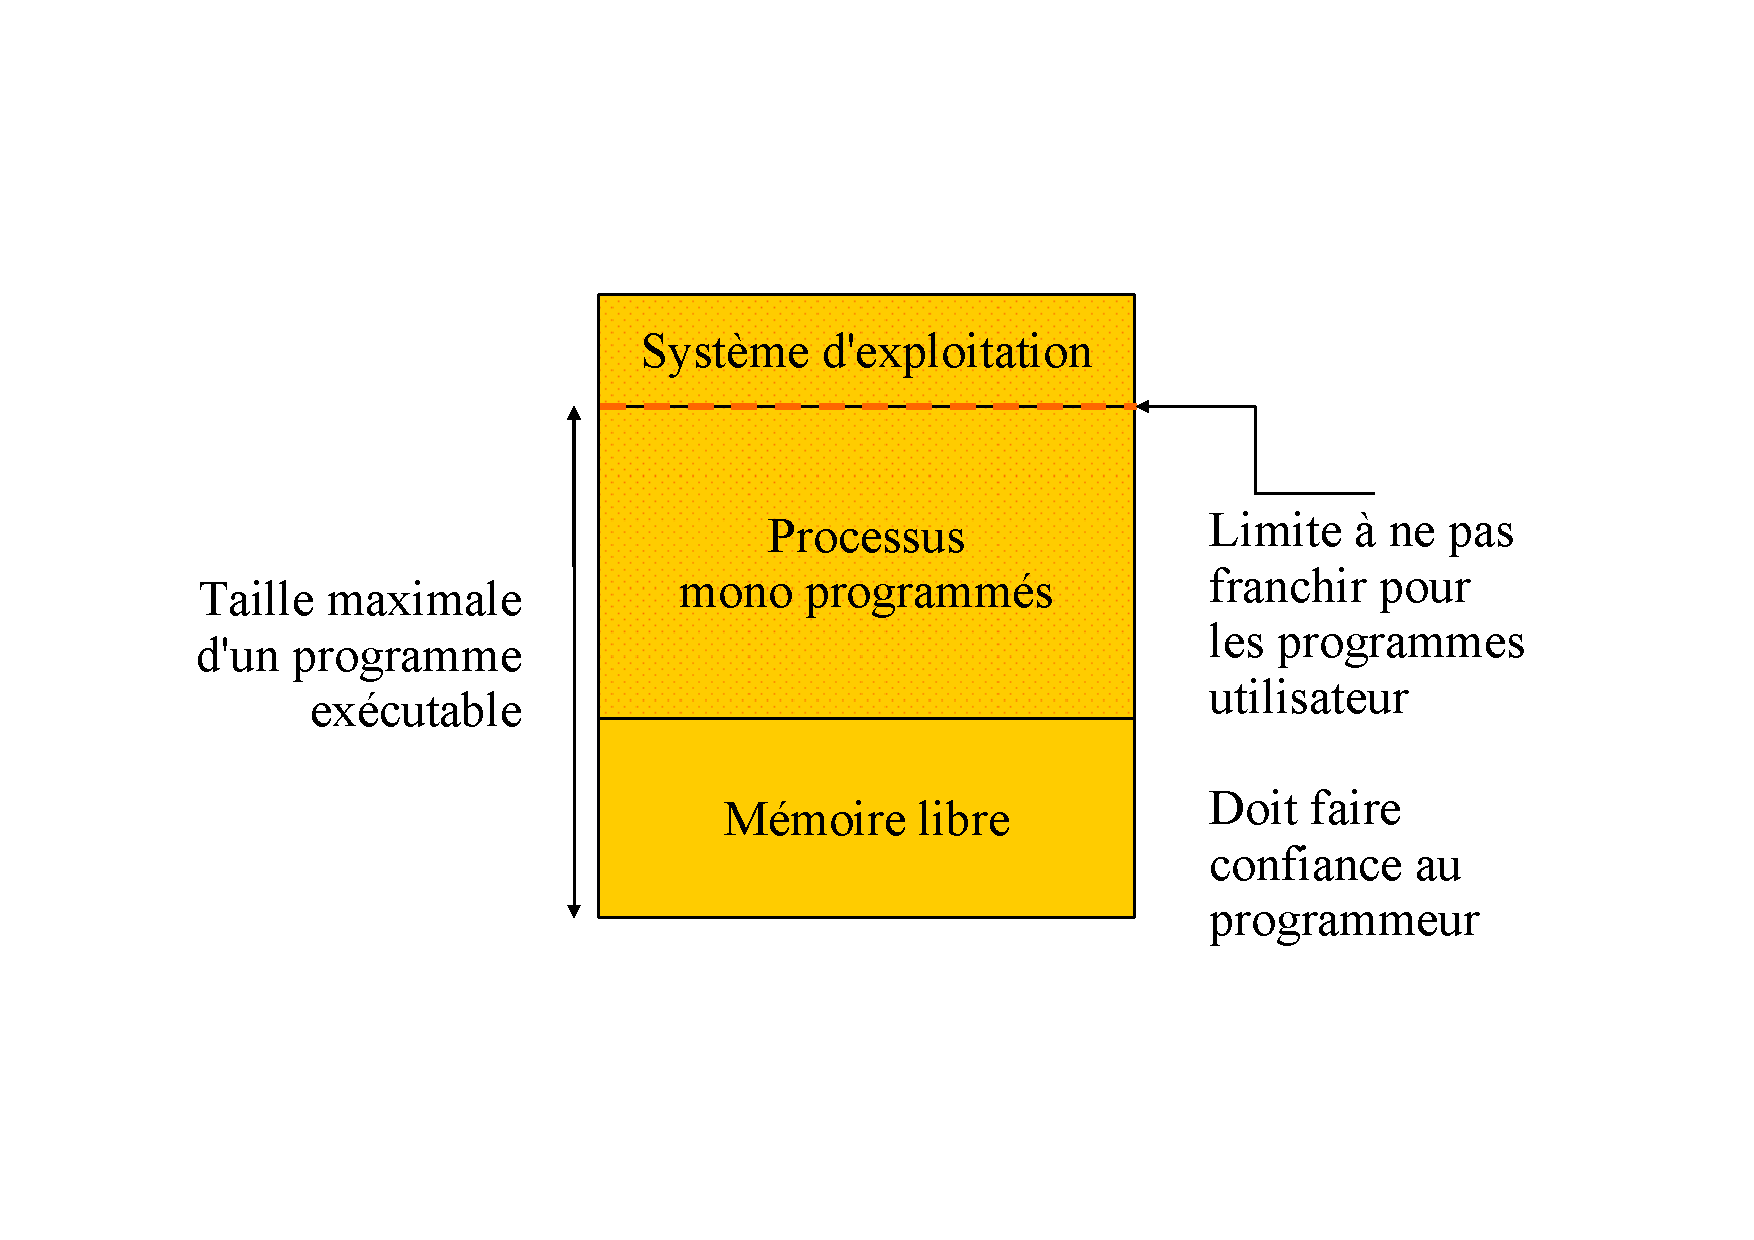
\includegraphics[width=.9\textwidth]{../illustration/memoire_principale_monoprogramme.pdf}
\end{frame}


\begin{frame}
\frametitle{L'unité de gestion de la mémoire}
\begin{itemize}
\item MMU : Memory Management Unit
\begin{itemize}
\item Périphérique matériel
\item Traduction adresse logique $\rightarrow$ adresse physique
\item Contrôle la validité de l'adresse logique
\item A la volée, pendant l'exécution de l'instruction
\end{itemize}
\item Plusieurs niveaux d'implémentation
\begin{itemize}
\item Registre de séparation, base et limite ou étendue
\item Segmentation, mémoire paginée...
\end{itemize}
\end{itemize}
\end{frame}



\begin{frame}
\frametitle{Registre de séparation}
\begin{itemize}
\item But :
\begin{itemize}
\item Séparer la mémoire système de la mémoire utilisateur
\end{itemize}
\item Registre de séparation :
\begin{itemize}
\item Contient l'adresse de la limite entre la zone système et la zone utilisateur
\end{itemize}
\item Calcul d'adresse effectué à la volée, pendant l'exécution 
\end{itemize}
\end{frame}

\begin{frame}
\frametitle{Registre de séparation}
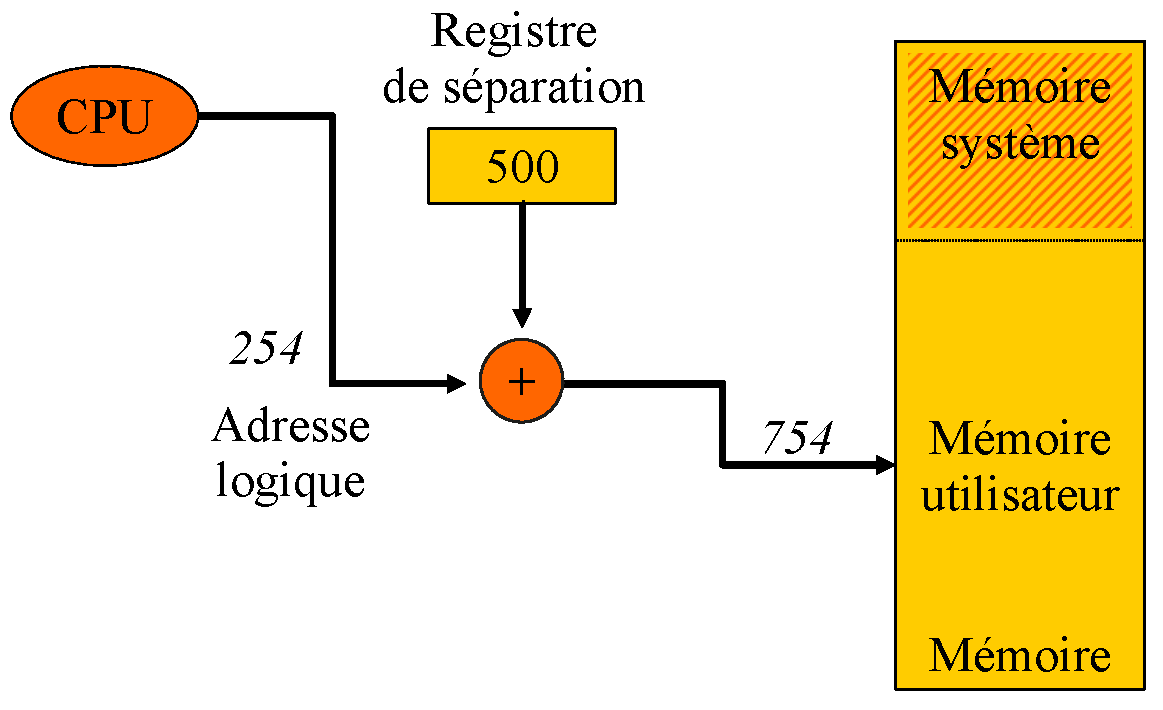
\includegraphics[width=\textwidth]{../illustration/memoire_principale_registre_sep.pdf}
\end{frame}


\begin{frame}
\frametitle{Registre base et étendue}
\begin{itemize}
\item Registre de base :
\begin{itemize}
\item Registre de base du processus
\begin{itemize}
\item Adresse physique du premier mot du programme
\end{itemize}
\item Adresse logique $\rightarrow$ adresse physique
\begin{itemize}
\item Adresse logique + valeur contenue dans le registre de translation
\item Translation d'adresse
\end{itemize}
\end{itemize}
\item Registre étendue :
\begin{itemize}
\item Taille zone mémoire du processus
\end{itemize}
\end{itemize}
\end{frame}


\begin{frame}
\frametitle{Registre base et étendue}
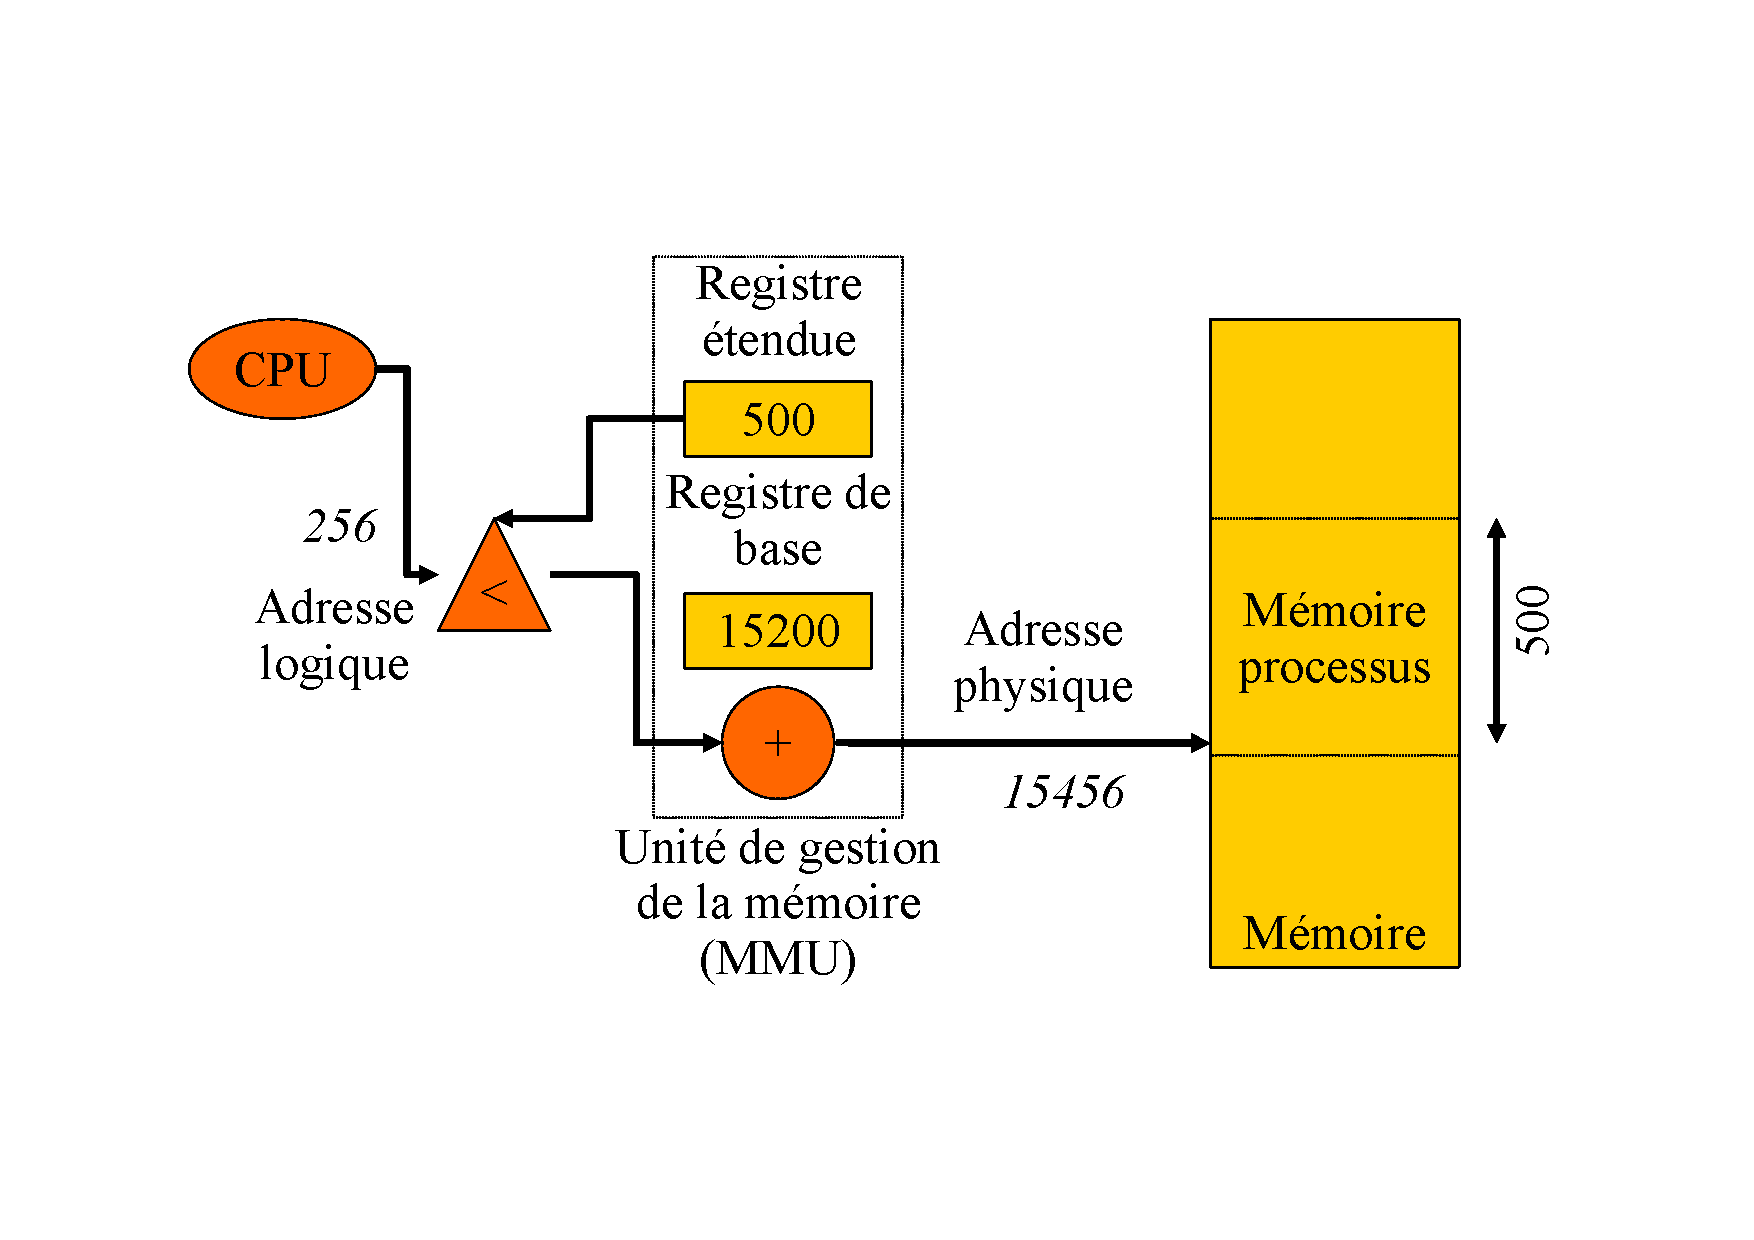
\includegraphics[width=\textwidth]{../illustration/memoire_principale_base_etendue.pdf}
\end{frame}


\begin{frame}
\frametitle{Registre base et étendue}
\begin{itemize}
\item Permet la partition de la mémoire entre les usagers
\begin{itemize}
\item Évite la propagation des erreurs entre processus
\item Autorise la multiprogrammation
\item Chargement des registres \textit{base} et \textit{étendue} à chaque commutation
\end{itemize}
\item Translation dynamique de processus
\begin{itemize}
\item Modification du registre de base
\end{itemize}
\end{itemize}
\end{frame}


\begin{frame}
\frametitle{Allocation mémoire}
\begin{itemize}
\item Avant et après le chargement d’un programme :
\begin{itemize}
\item Allocation mémoire par le système
\item Libération à la fin du programme
\item Possibilité d'allocation et de libération dynamique
\end{itemize}
\item Nécessité de connaître l'état mémoire
\begin{itemize}
\item Zones libres et occupées
\end{itemize}
\item Exploitation de :
\begin{itemize}
\item Stratégie d’allocation
\item Procédures de libération
\end{itemize}
\end{itemize}
\end{frame}

\begin{frame}
\frametitle{État de la mémoire}
\begin{itemize}
\item État des emplacements occupés de la mémoire
\item Solutions possibles :
\begin{itemize}
\item Table de bits
\item Liste chaînée
\item Subdivisions
\end{itemize}
\item La mémoire découpée :
\begin{itemize}
\item En unités (blocs d’allocation)
\end{itemize}
\end{itemize}
\end{frame}


\begin{frame}
\frametitle{Représentation de l'état mémoire par table de bits}
\begin{itemize}
\item Tableau de bits
\begin{itemize}
\item Représente l'état des blocs de mémoire
\end{itemize}
\item Unités libres notées par 0
\begin{itemize}
\item Unités occupées par un 1 (ou inverse)
\item Simple à implanter
\end{itemize}
\item Peu performant
\begin{itemize}
\item occupation mémoire
\item coût de parcours
\end{itemize}
\end{itemize}
\end{frame}


\begin{frame}
\frametitle{Représentation de l'état mémoire par table de bits}
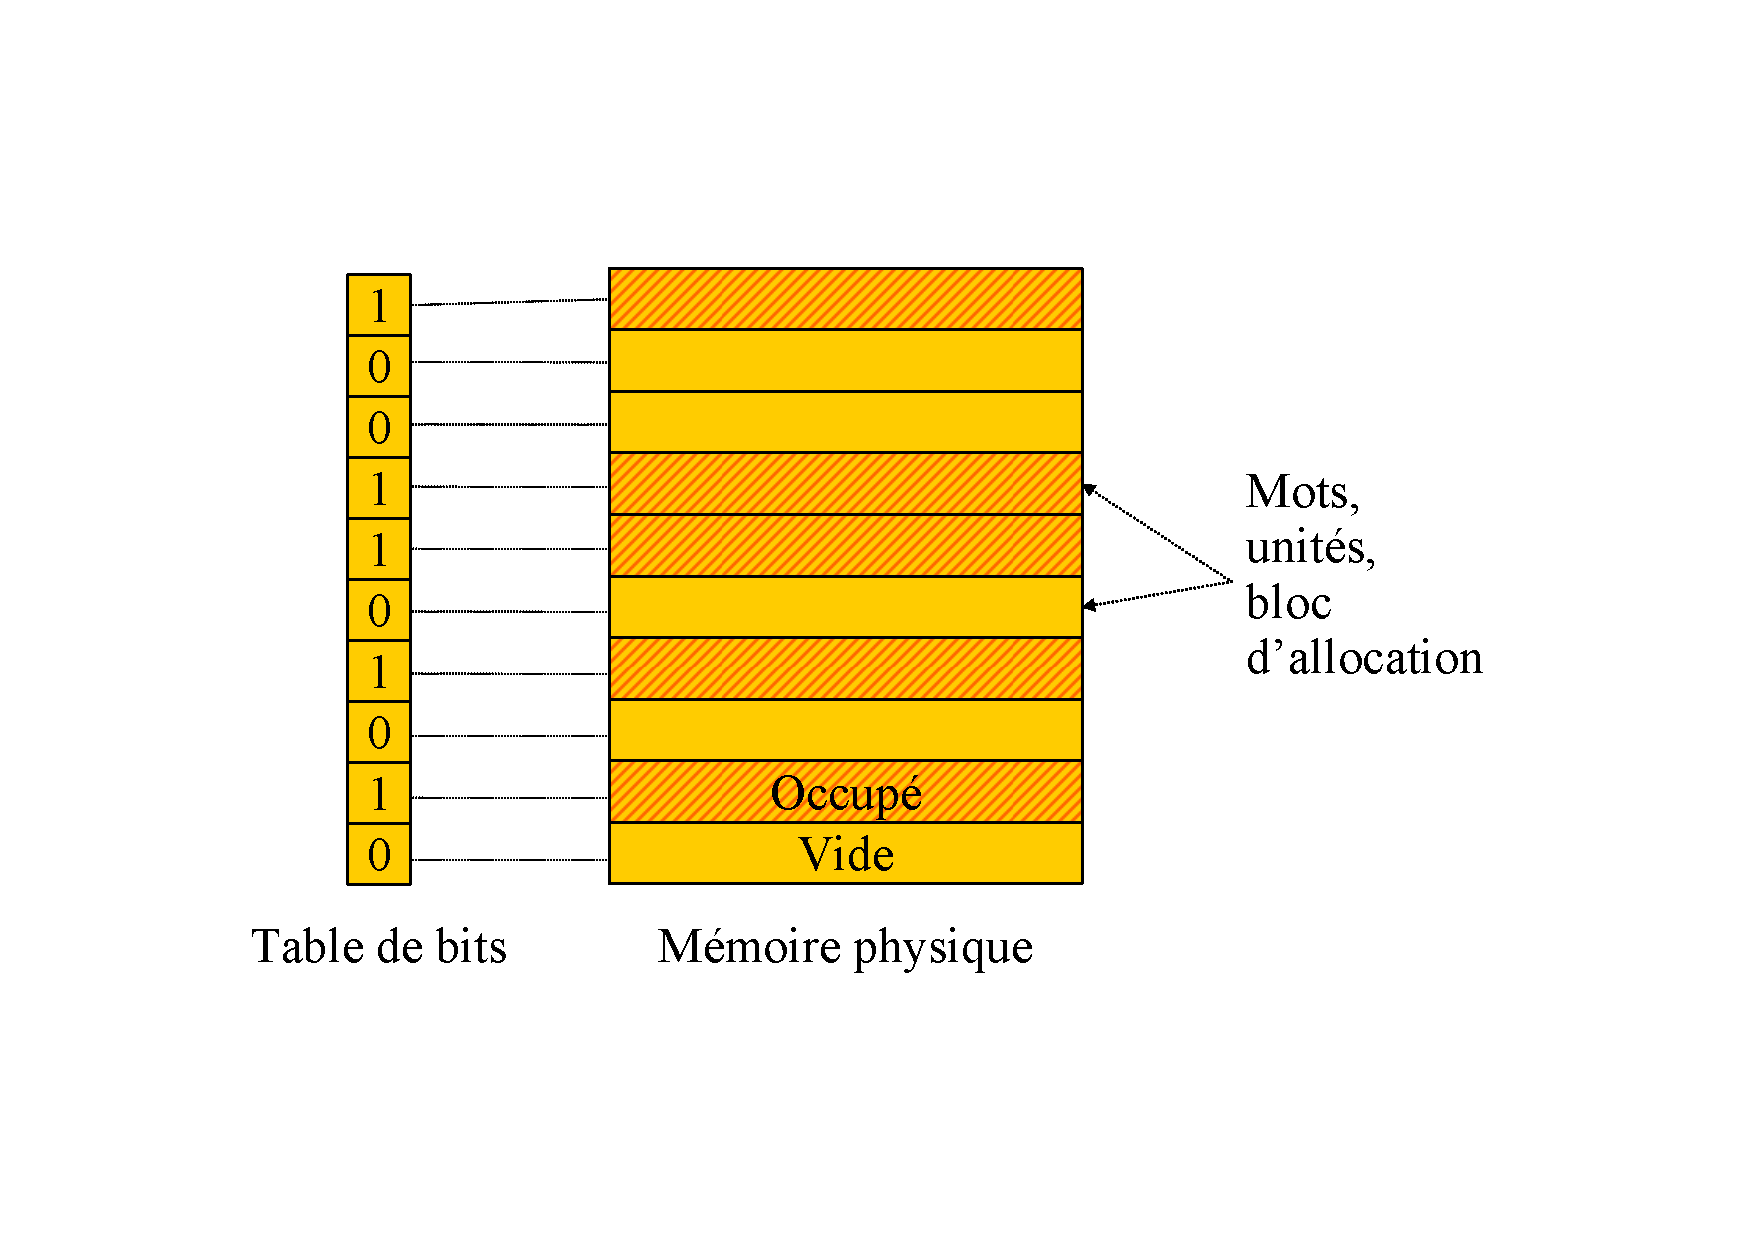
\includegraphics[width=.9\textwidth]{../illustration/memoire_principale_table_bit.pdf}
\end{frame}


\begin{frame}
\frametitle{Représentation de l'état mémoire par table de bits}
\begin{itemize}
\item Difficile à dimensionner
\begin{itemize}
\item Unité d’allocation petite :
\begin{itemize}
\item Moins de pertes lors des allocations
\item Table d ’allocation volumineuse
\end{itemize}
\item Unité d'allocation grande :
\begin{itemize}
\item Utilisation moins efficace de la mémoire
\item Table d'allocation plus compacte
\end{itemize}
\end{itemize}
\item Taille fixe quelle que soit l’occupation mémoire
\item Méthode peu utilisée
\end{itemize}
\end{frame}


\begin{frame}
\frametitle{Représentation de l'état mémoire par listes chaînées}
\begin{itemize}
\item Mémoire : liste chaînée dont chaque élément porte :
\begin{itemize}
\item Type (libre ou occupé)
\item Adresse de début
\item Longueur
\item Pointeur sur l’élément suivant
\end{itemize}
\item Utilisation possible d'une des deux listes :
\begin{itemize}
\item Une pour les zones libres
\item Une pour les zones utilisées
\end{itemize}
\end{itemize}
\end{frame}


\begin{frame}
\frametitle{Représentation de l'état mémoire par listes chaînées}
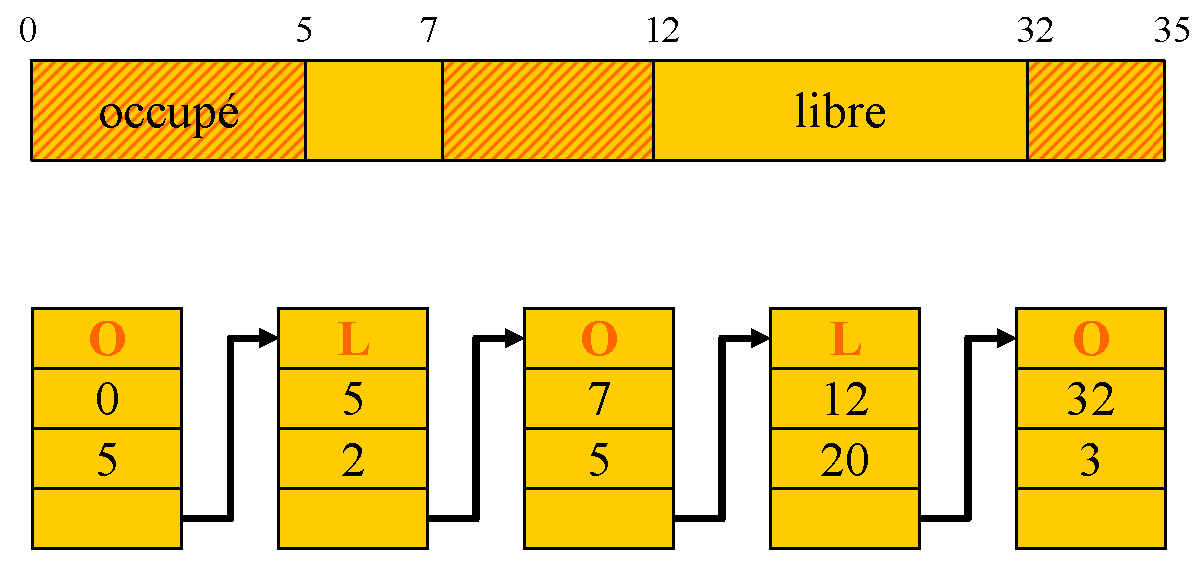
\includegraphics[width=\textwidth]{../illustration/memoire_principale_liste_chainee.pdf}
\end{frame}


\begin{frame}
\frametitle{Représentation de l'état mémoire par listes chaînées}
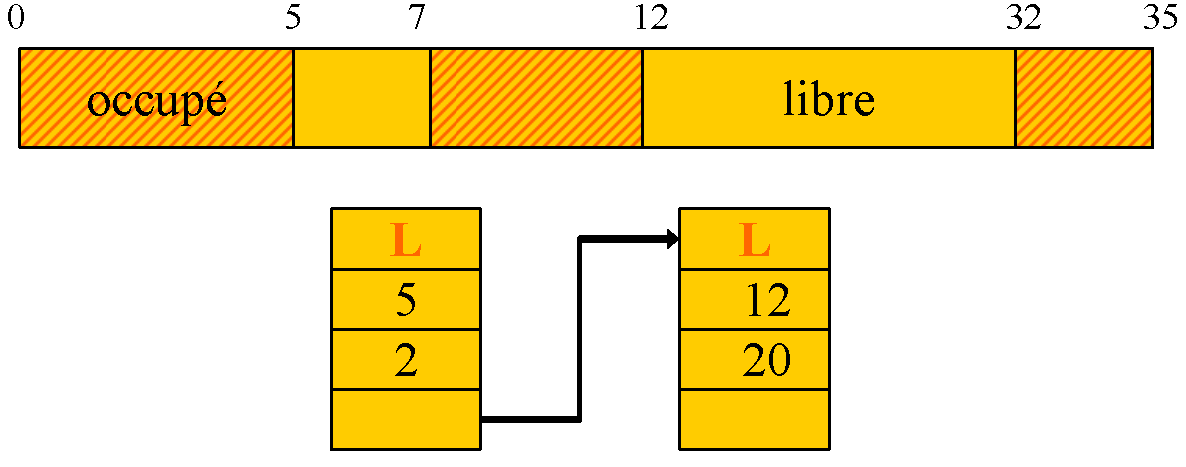
\includegraphics[width=\textwidth]{../illustration/memoire_principale_liste_chainee2.pdf}
\end{frame}


\begin{frame}
\frametitle{Allocation de partitions de taille variable}
\begin{itemize}
\item Partition :
\begin{itemize}
\item Segment de mémoire attribué à un processus
\item Taille variable en fonction de la demande
\end{itemize}
\item Partition éventuellement translatables
\item Déplacement dynamique en cours d'exécution
\begin{itemize}
\item Changement de l'adresse de base de la partition
\end{itemize}
\end{itemize}
\end{frame}


\begin{frame}
\frametitle{Politiques d’allocation}
\begin{itemize}
\item Recherche un espace libre pour un processus
\item Quatre stratégies possibles :
\begin{itemize}
\item Premier ajustement
\item Meilleur ajustement
\item Pire ajustement
\item Méthode des subdivisions
\end{itemize}
\end{itemize}
\end{frame}

\begin{frame}
\frametitle{Politique du premier ajustement}
\begin{columns}
\column{0.6\textwidth}
\begin{itemize}
\item Premier bloc libre de la liste pouvant contenir la partition demandée
\item La recherche peut débuter :
\begin{itemize}
\item Au début de la mémoire
\item A l'endroit de la dernière allocation
\end{itemize}
\end{itemize}
\column{0.4\textwidth}
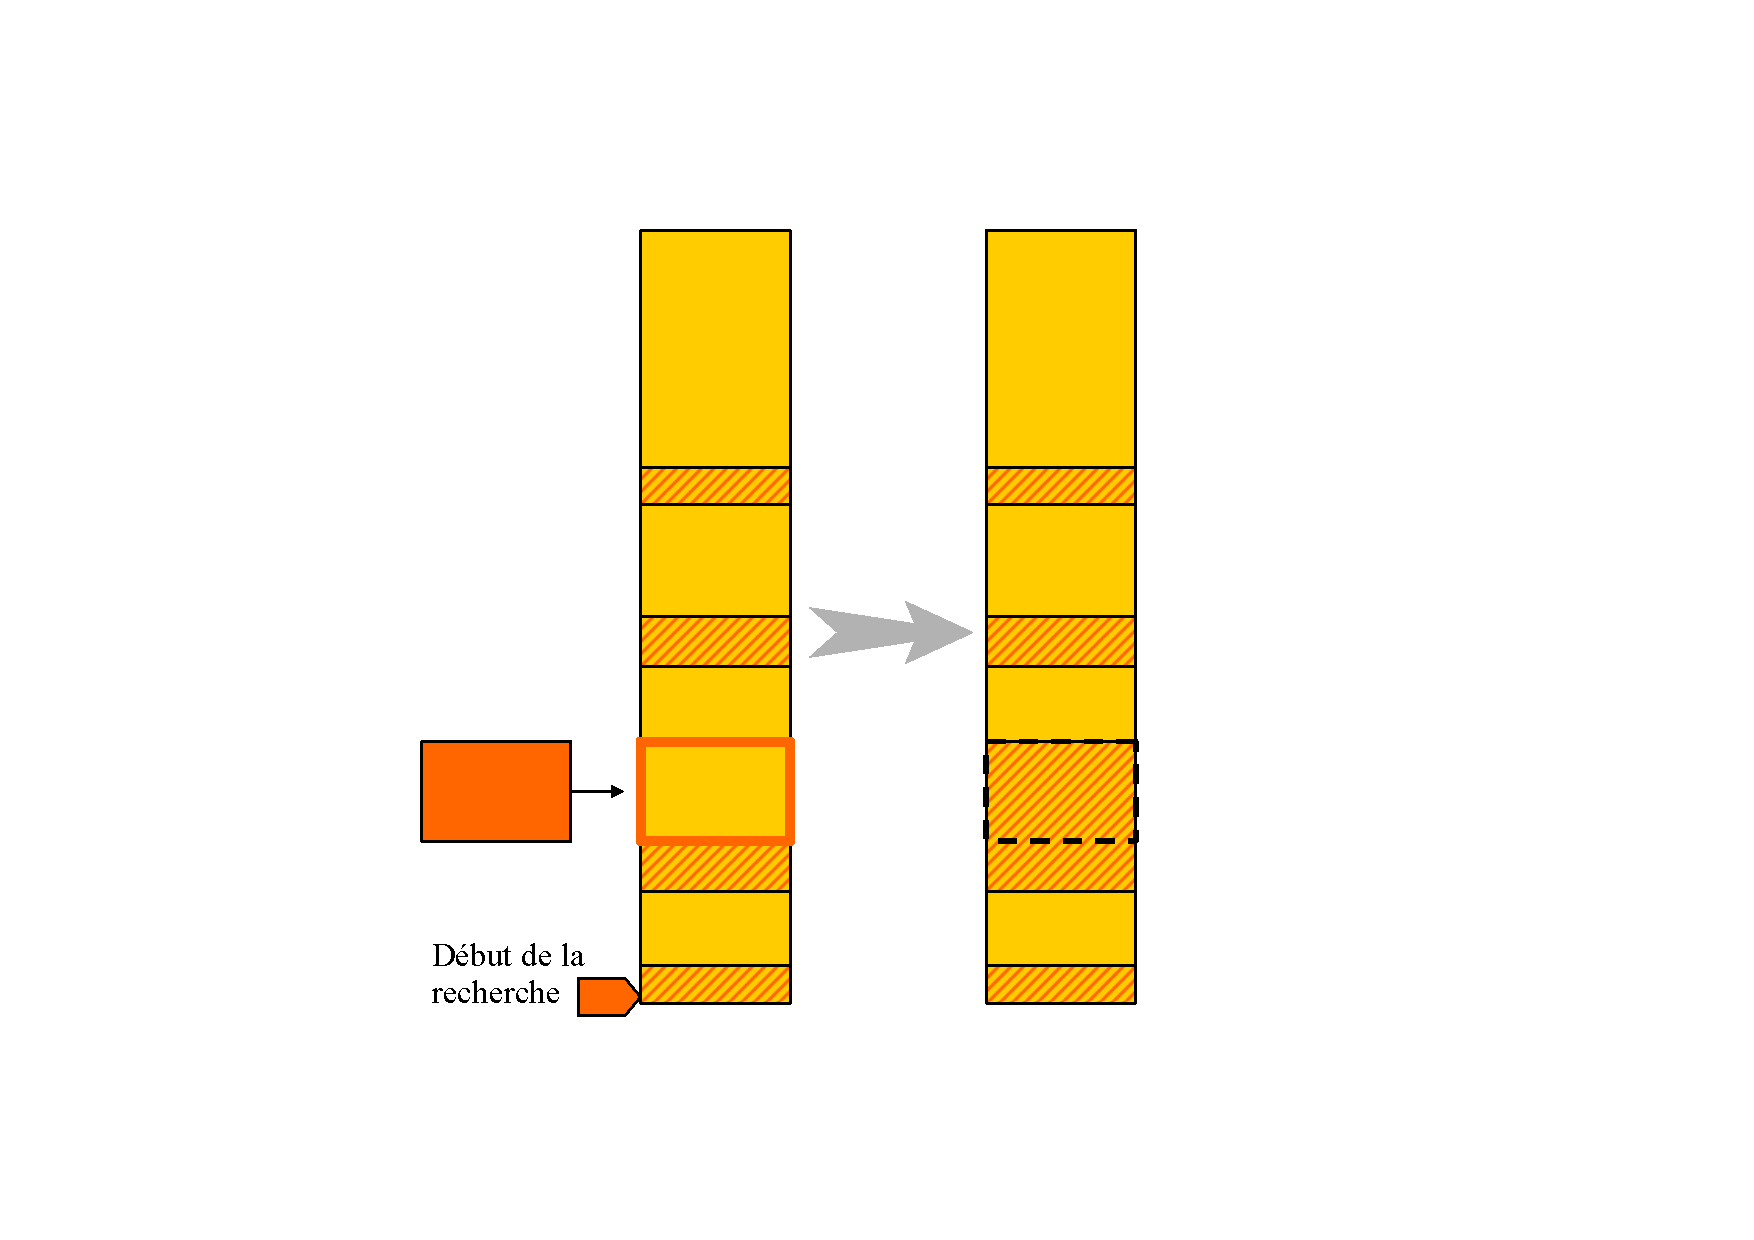
\includegraphics[height=.6\textheight]{../illustration/memoire_principale_premier_ajustement.pdf}
\end{columns}
\end{frame}


\begin{frame}
\frametitle{Politique du premier ajustement}
\begin{itemize}
\item Économique - rapide
\begin{itemize}
\item parcours mémoire limité
\end{itemize}
\item Pas de contrôle de l'occupation mémoire
\end{itemize}
\end{frame}


\begin{frame}
\frametitle{Politique du meilleur ajustement}
\begin{itemize}
\item Tente d’allouer au processus l’espace mémoire le plus petit qui puisse contenir le processus
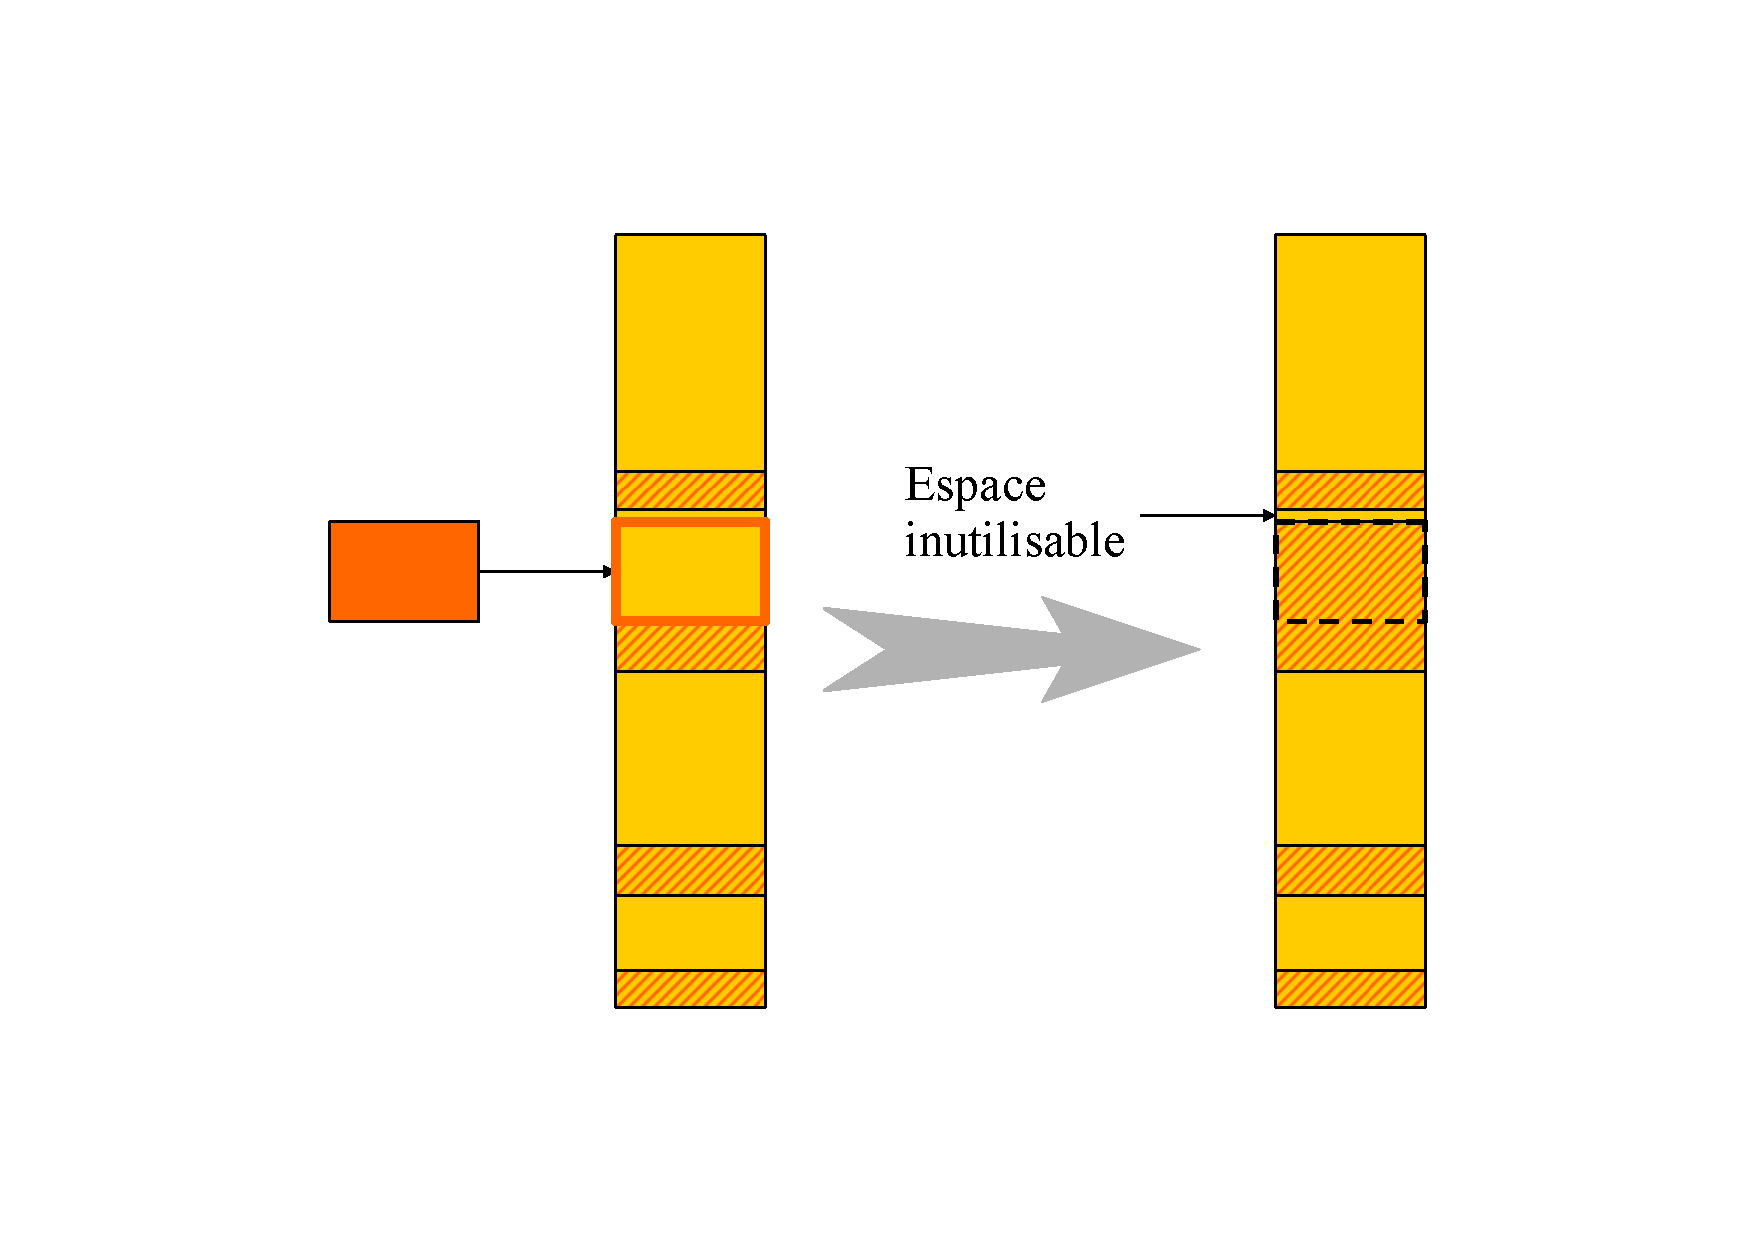
\includegraphics[width=.7\textwidth]{../illustration/memoire_principale_meilleur_ajustement.pdf}
\end{itemize}
\end{frame}


\begin{frame}
\frametitle{Politique du meilleur ajustement}
\begin{itemize}
\item Algorithme coûteux
\begin{itemize}
\item parcours de toute la mémoire
\end{itemize}
\item Génère une importante fragmentation
\begin{itemize}
\item création de petits espaces inutilisables
\item fragmentation externe
\end{itemize}
\end{itemize}
\end{frame}


\begin{frame}
\frametitle{Politique du pire ajustement}
Recherche le plus grand bloc d ’espace mémoire disponible

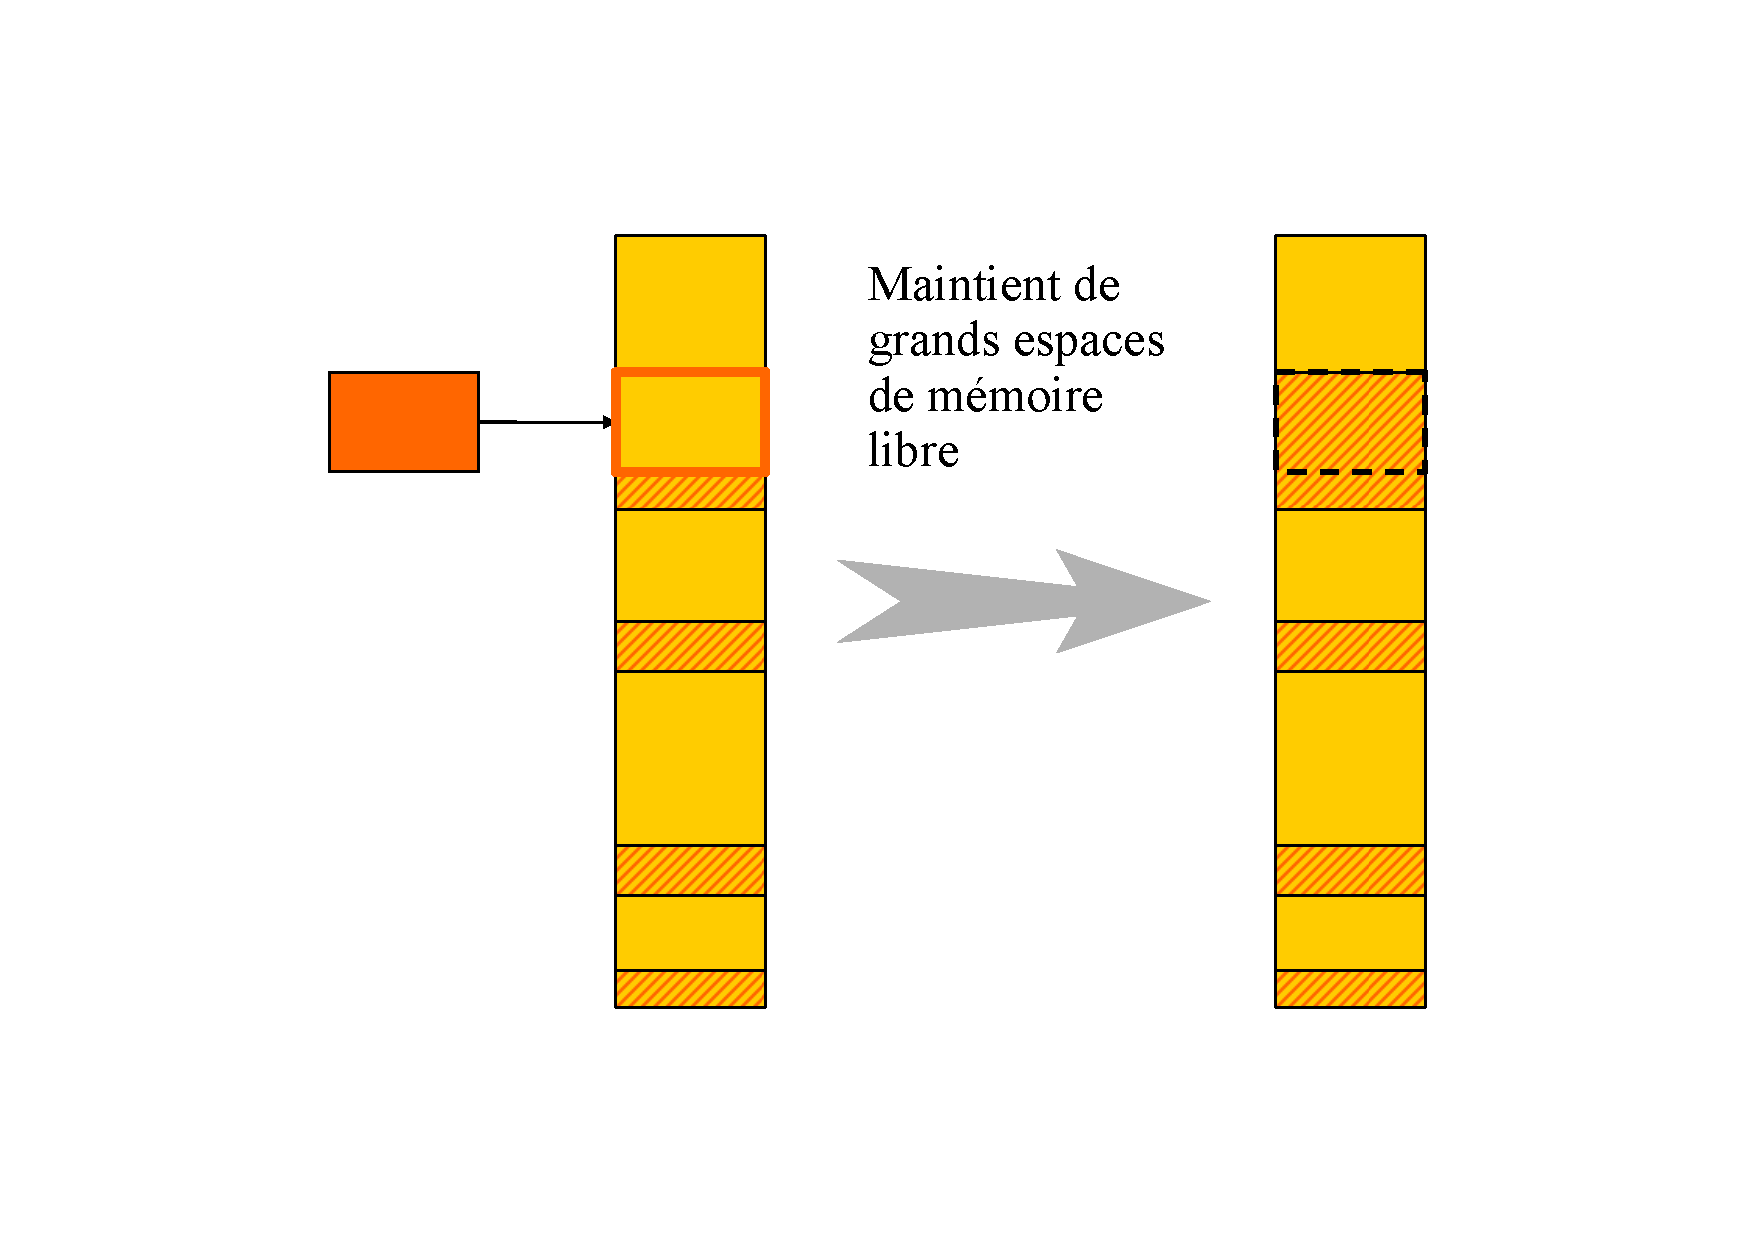
\includegraphics[width=.7\textwidth]{../illustration/memoire_principale_pire_ajustement.pdf}
\end{frame}


\begin{frame}
\frametitle{Politique du pire ajustement}
\begin{itemize}
\item Algorithme coûteux
\begin{itemize}
\item Parcours de toute la mémoire
\end{itemize}
\item Limite le fractionnement
\begin{itemize}
\item Laisse de grands espace de mémoire libres
\item Espaces utilisables pour les autres données
\end{itemize}
\end{itemize}
\end{frame}



\begin{frame}
\frametitle{Choix algorithme d’allocation}
\begin{itemize}
\item Algorithme du pire ajustement le plus élégant
\begin{itemize}
\item Limite le fractionnement
\item Laisse de grands espaces mémoire disponibles
\end{itemize}
\item Algorithme du premier ajustement le plus efficace en pratique (simulations)
\begin{itemize}
\item Parcours mémoire limité
\item Limite le temps de recherche
\end{itemize}
\end{itemize}
\end{frame}


\begin{frame}
\frametitle{Méthode des subdivisions (buddy-system)}
\begin{itemize}
\item Introduit par Donald KNUTH en 1973
\item Encore appelée méthode des frères siamois
\item Subdivisions successives de la mémoire par dichotomie jusqu'à trouver un emplacement mémoire adapté
\item Fragment initial de la taille de la mémoire (puissance de 2)
\end{itemize}
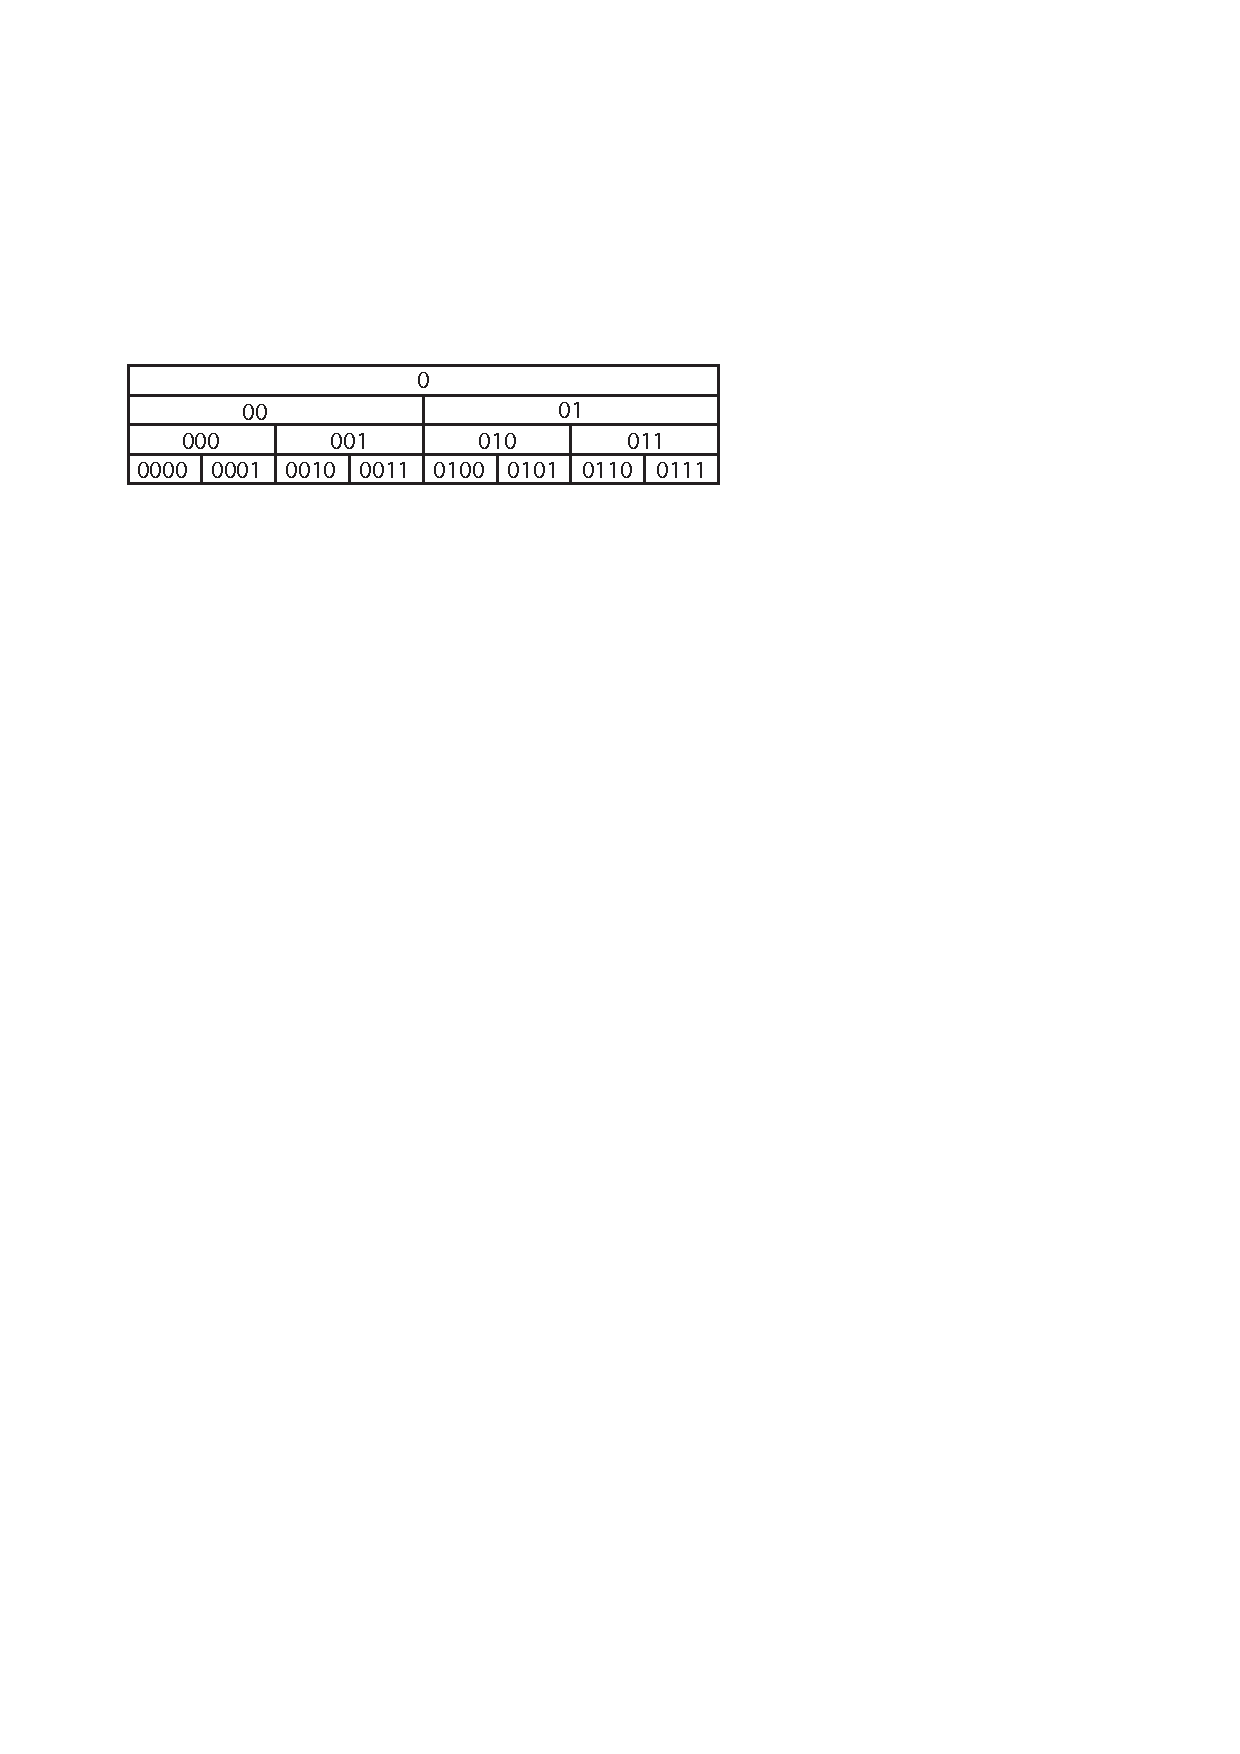
\includegraphics[width=\textwidth]{../illustration/buddy.pdf}
\end{frame}


\begin{frame}
\frametitle{Récupération de mémoire}
Libération manuelle :
\begin{itemize}
\item Appel système (free)
\item Source d’erreurs
\item Risque de fuite de mémoire (memory leak)
\begin{itemize}
\item Oubli de libération de segments alloués
\item Segments inutilisables pour les autres processus
\end{itemize}
\end{itemize}
\end{frame}


\begin{frame}
\frametitle{Libération de mémoire}
\begin{itemize}
\item Évacuation d'un processus de la mémoire
\item Libération des blocs utilisés
\begin{itemize}
\item Marquage à libre
\item Fusion avec les blocs libres adjacents
\end{itemize}
\end{itemize}
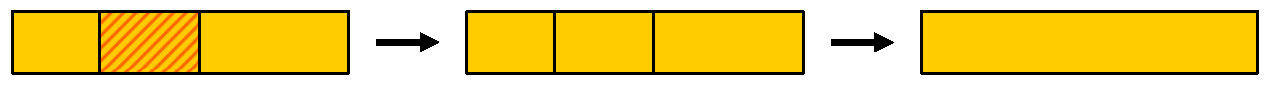
\includegraphics[width=\textwidth]{../illustration/memoire_principale_liberation_bloc.pdf}
\end{frame}


\begin{frame}
\frametitle{Récupération de mémoire}
\begin{itemize}
\item Fragmentation externe de la mémoire
\begin{itemize}
\item Sature l’espace disponible
\item Nécessite un compactage régulier
\item Déplacement des partitions
\begin{itemize}
\item Vers de bas de la mémoire
\item Création bloc libre en haut de mémoire
\end{itemize}
\end{itemize}

\item Algorithme coûteux
\item Nécessite des segments translatables
\end{itemize}
\end{frame}

\begin{frame}
\frametitle{Récupération de mémoire}
\begin{itemize}
\item Ramasse miettes (garbage collector)
\item Stop and copy :
\begin{itemize}
\item Tâche de basse priorité
\item Récupération de mémoire asynchrone
\begin{itemize}
\item Arrêt des processus
\item Balaye des objets mémoire
\item Repère objets non référencés par pointeur valide
\item Marquage à libre emplacements correspondants
\item Compactage mémoire libre (déplacement zones en cours d’utilisation)
\end{itemize}
\item Récupération de mémoire synchrone possible
\end{itemize}
\item Coûteux
\end{itemize}
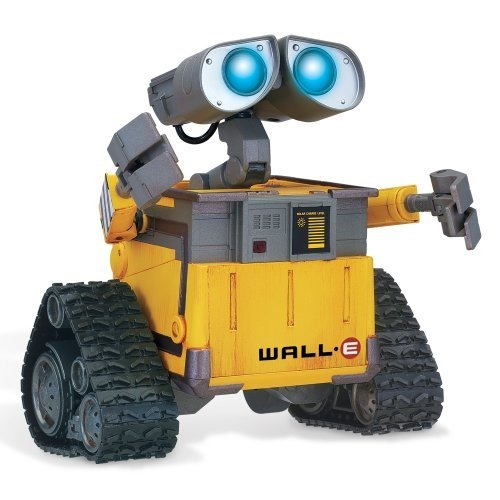
\includegraphics[width=2cm]{../illustration/wall-e.jpg}
\end{frame}

%-----------------------------------------------
\subsection{La segmentation}
%-----------------------------------------------
\begin{frame}
\frametitle{La segmentation}
Programme généralement constitué de plusieurs entités logiques:
\begin{itemize}
\item Programme principal
\begin{itemize}
\item procédures
\item fonctions bibliothèques
\item tables de données...
\end{itemize}
\item Séparation de ces entités en segments
\begin{itemize}
\item Un segment = une partition
\end{itemize}
\end{itemize}
\end{frame}


\begin{frame}
\frametitle{Les politiques d'allocation}
\begin{itemize}
\item Segmentation
\item Pagination
\item Segmentation paginée
\end{itemize}
\end{frame}


\begin{frame}
\frametitle{La segmentation}
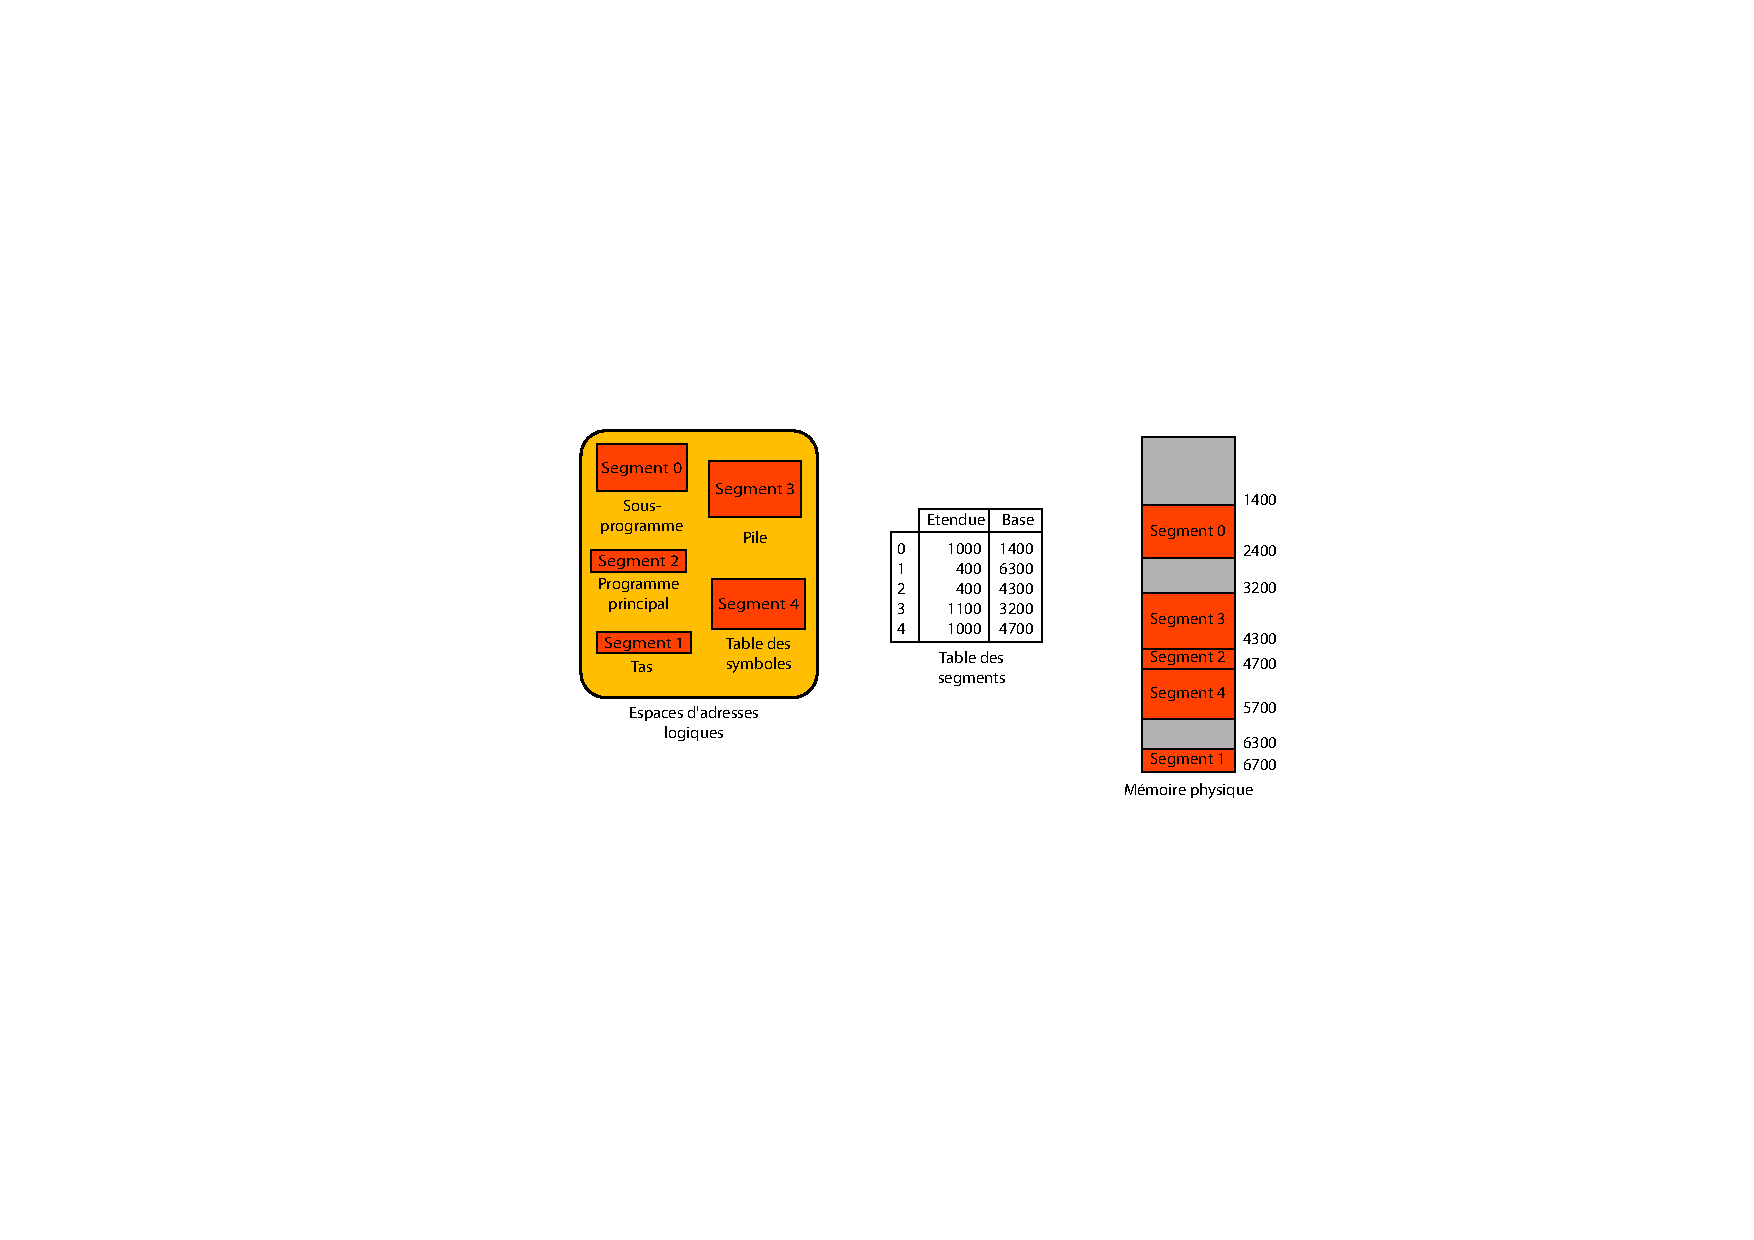
\includegraphics[width=\textwidth]{../illustration/memoire_segment_exemple.pdf}
\end{frame}


\begin{frame}
\frametitle{La segmentation}
\begin{itemize}
\item Calcul d'adresse dans un environnement segmenté :
\begin{itemize}
\item Numéro de segment
\item Déplacement dans ce segment
\end{itemize}
\item Type de segmentation :
\begin{itemize}
\item Globale, valable pour l'ensemble du système
\item Locale à un processus
\end{itemize}
\end{itemize}
\end{frame}


\begin{frame}
\frametitle{Calcul adresse segmentation}
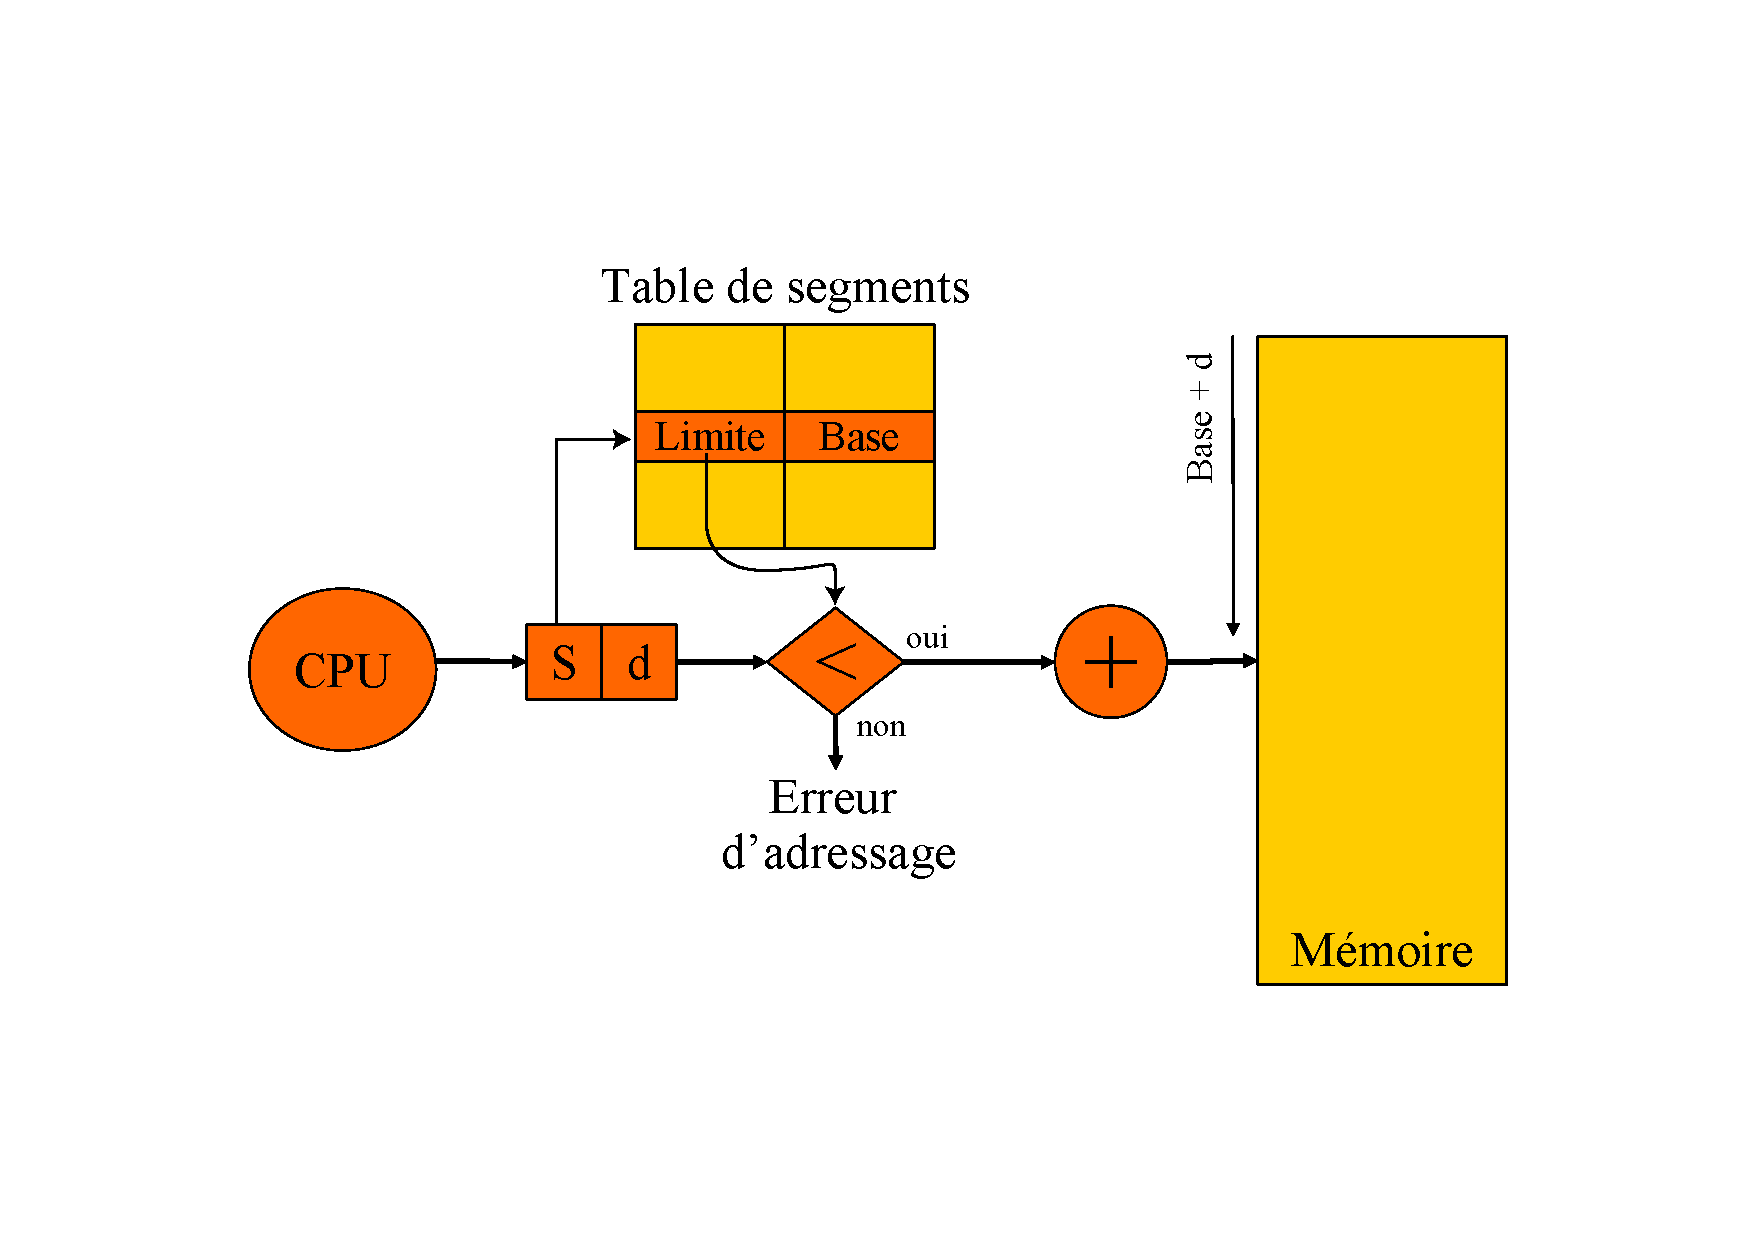
\includegraphics[width=.9\textwidth]{../illustration/memoire_segment_acces.pdf}
\end{frame}


\begin{frame}
\frametitle{Implantation de la table des segments }
Plusieurs mécanismes :
\begin{itemize}
\item Registres spécialisés changés à chaque commutation
\begin{itemize}
\item Rapide mais uniquement s'il y a peu de segments
\end{itemize}
\item Segment mémoire contenant la table des segments plus un registre pointant vers ce dernier
\begin{itemize}
\item Deux accès mémoire pour calcul d'adresse
\end{itemize}
\item Ensemble de registres pour les segments les plus souvent référencés
\begin{itemize}
\item Mécanisme de cache
\end{itemize}
\end{itemize}
\end{frame}

\begin{frame}
\frametitle{Segmentation}
\begin{columns}
\column{0.5\textwidth}
\begin{block}{Avantages}
\begin{itemize}
\item Facilite l'allocation de mémoire (plus petits)
\item Facilite le partage de données et de code
\begin{itemize}
\item Partage de segment
\end{itemize}
\item Protection des segments entre eux
\end{itemize}
\end{block}
\column{0.5\textwidth}
\begin{block}{Inconvénients}
\begin{itemize}
\item Chaque segment doit être une portion de mémoire contiguë
\item Impossible de fractionner les segments
\item Fragmentation externe
\end{itemize}
\end{block}
\end{columns}
\end{frame}



\begin{frame}
\frametitle{Pagination}
\begin{itemize}
\item Permet aux processus et données d'utiliser des adresses non contiguës
\item Découpage mémoire physique en partitions de taille fixe appelées cases ou cadres
\item Découpage de la mémoire linéaire des processus en partitions appelées pages
\begin{itemize}
\item Pages et cases de même taille (4 Ko sur x86)
\item Correspondance page $\Leftrightarrow$ case
\end{itemize}
\end{itemize}
\end{frame}


\begin{frame}
\frametitle{Représentation de l'espace d'adressage paginé}
\begin{itemize}
\item La \textbf{page} est la partie \textbf{virtuelle} de la mémoire,
\item Le \textbf{cadre} (ou case) est la partie \textbf{physique} de la mémoire
\item Correspondance entre case et page
\end{itemize}
\end{frame}

\begin{frame}
\frametitle{Principe de la pagination}
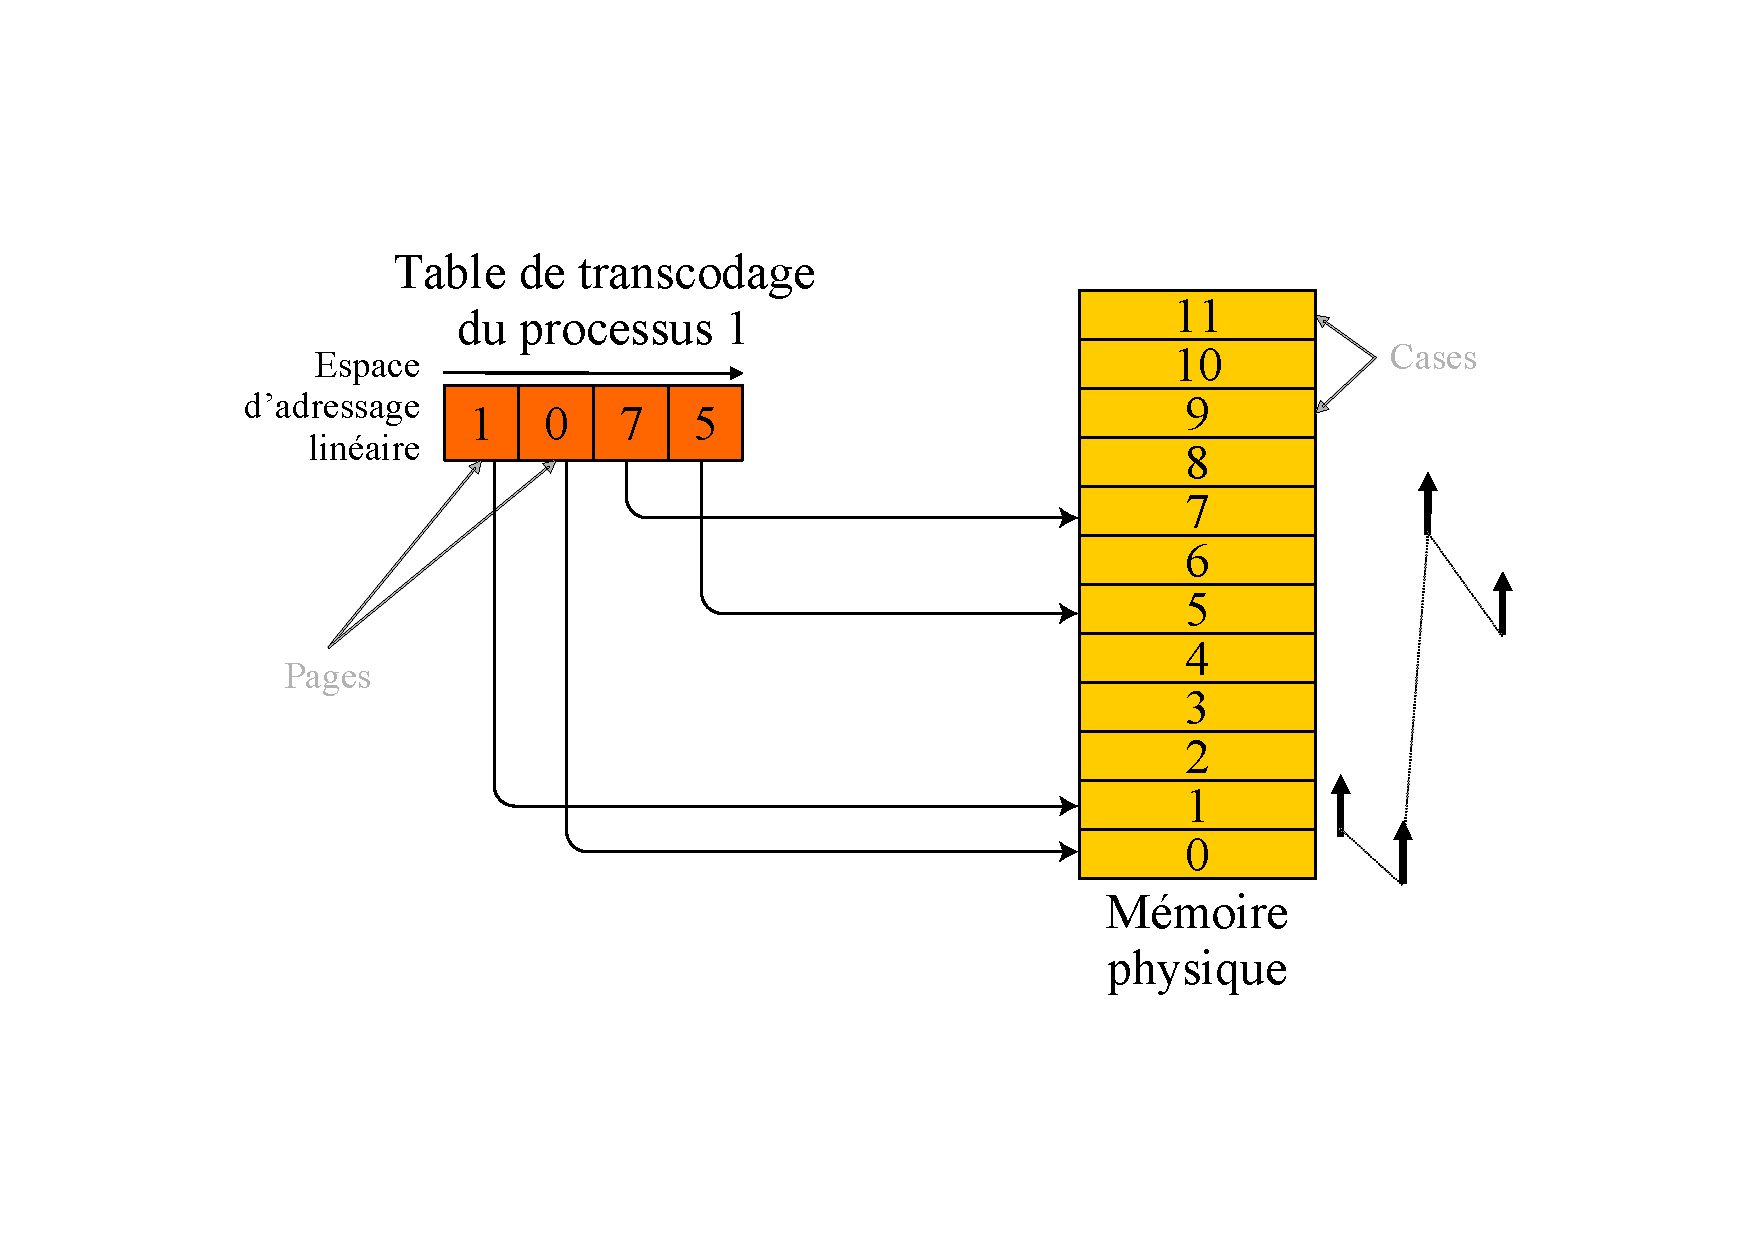
\includegraphics[width=.9\textwidth]{../illustration/memoire_paginee_acces.pdf}
\end{frame}

\begin{frame}
\frametitle{La pagination}
\begin{itemize}
\item Supprime le problème du fractionnement externe de la mémoire
\item Allocation mémoire à un processus :
\begin{itemize}
\item Attribution de pages
\item Possible en cours d'exécution (allocation dynamique)
\end{itemize}
\item Libération de mémoire :
\begin{itemize}
\item Libération de page
\end{itemize}
\end{itemize}
\end{frame}


\begin{frame}
\frametitle{La pagination}
\begin{itemize}
\item Adresse en mémoire paginée :
\begin{itemize}
\item Numéro de page + déplacement dans la page
\end{itemize}
\end{itemize}
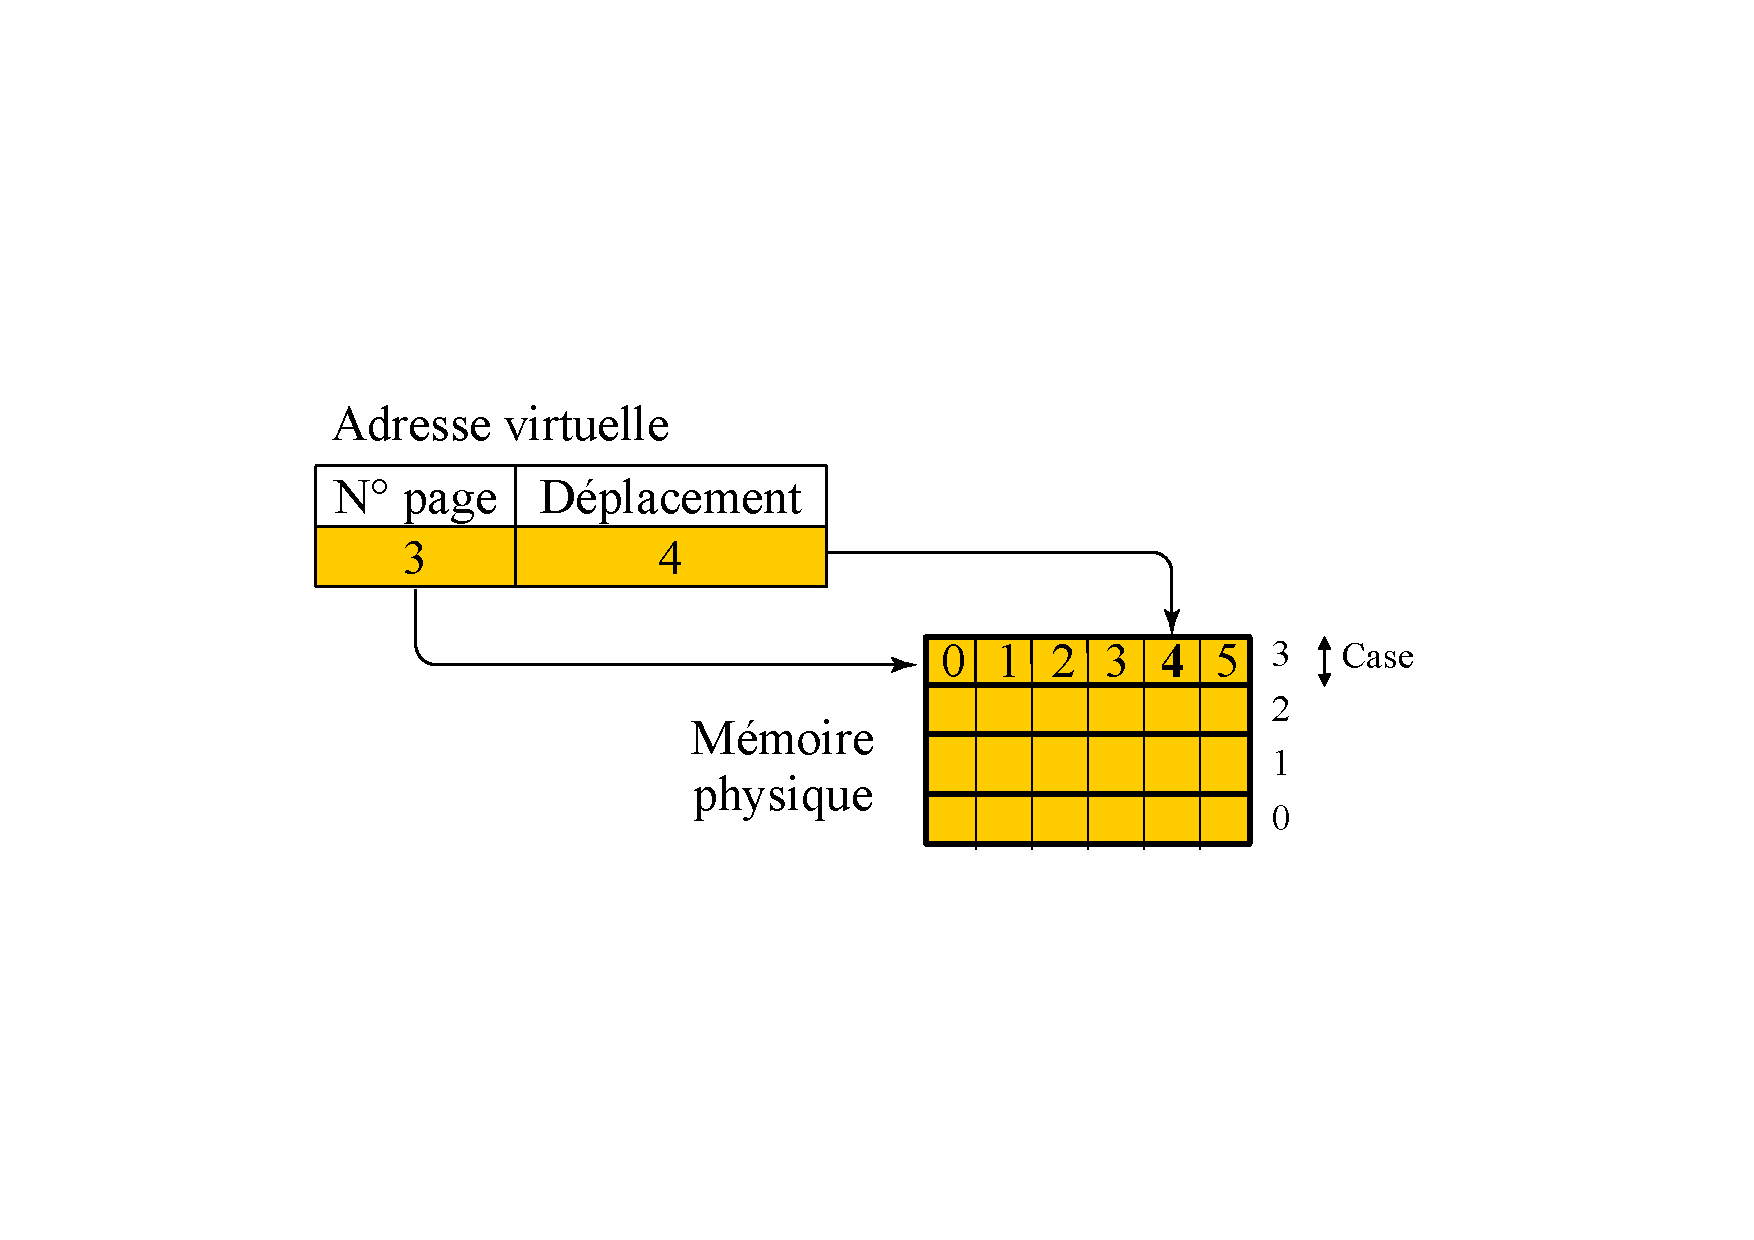
\includegraphics[width=.9\textwidth]{../illustration/memoire_paginee_deplacement.pdf}
\end{frame}


\begin{frame}
\frametitle{Table de transcodage processus}
\begin{itemize}
\item Permet de faire la correspondance entre le numéro de page et le numéro de case
\begin{itemize}
\item transformation adresse virtuelle (page) en adresse réelle (case)
\end{itemize}
\item Les pages dont le numéro n'apparaît pas dans la table de transcodage du processus lui sont inaccessibles
\begin{itemize}
\item protection mémoire
\end{itemize}
\end{itemize}
\end{frame}

\begin{frame}
\frametitle{Table de transcodage du processus}
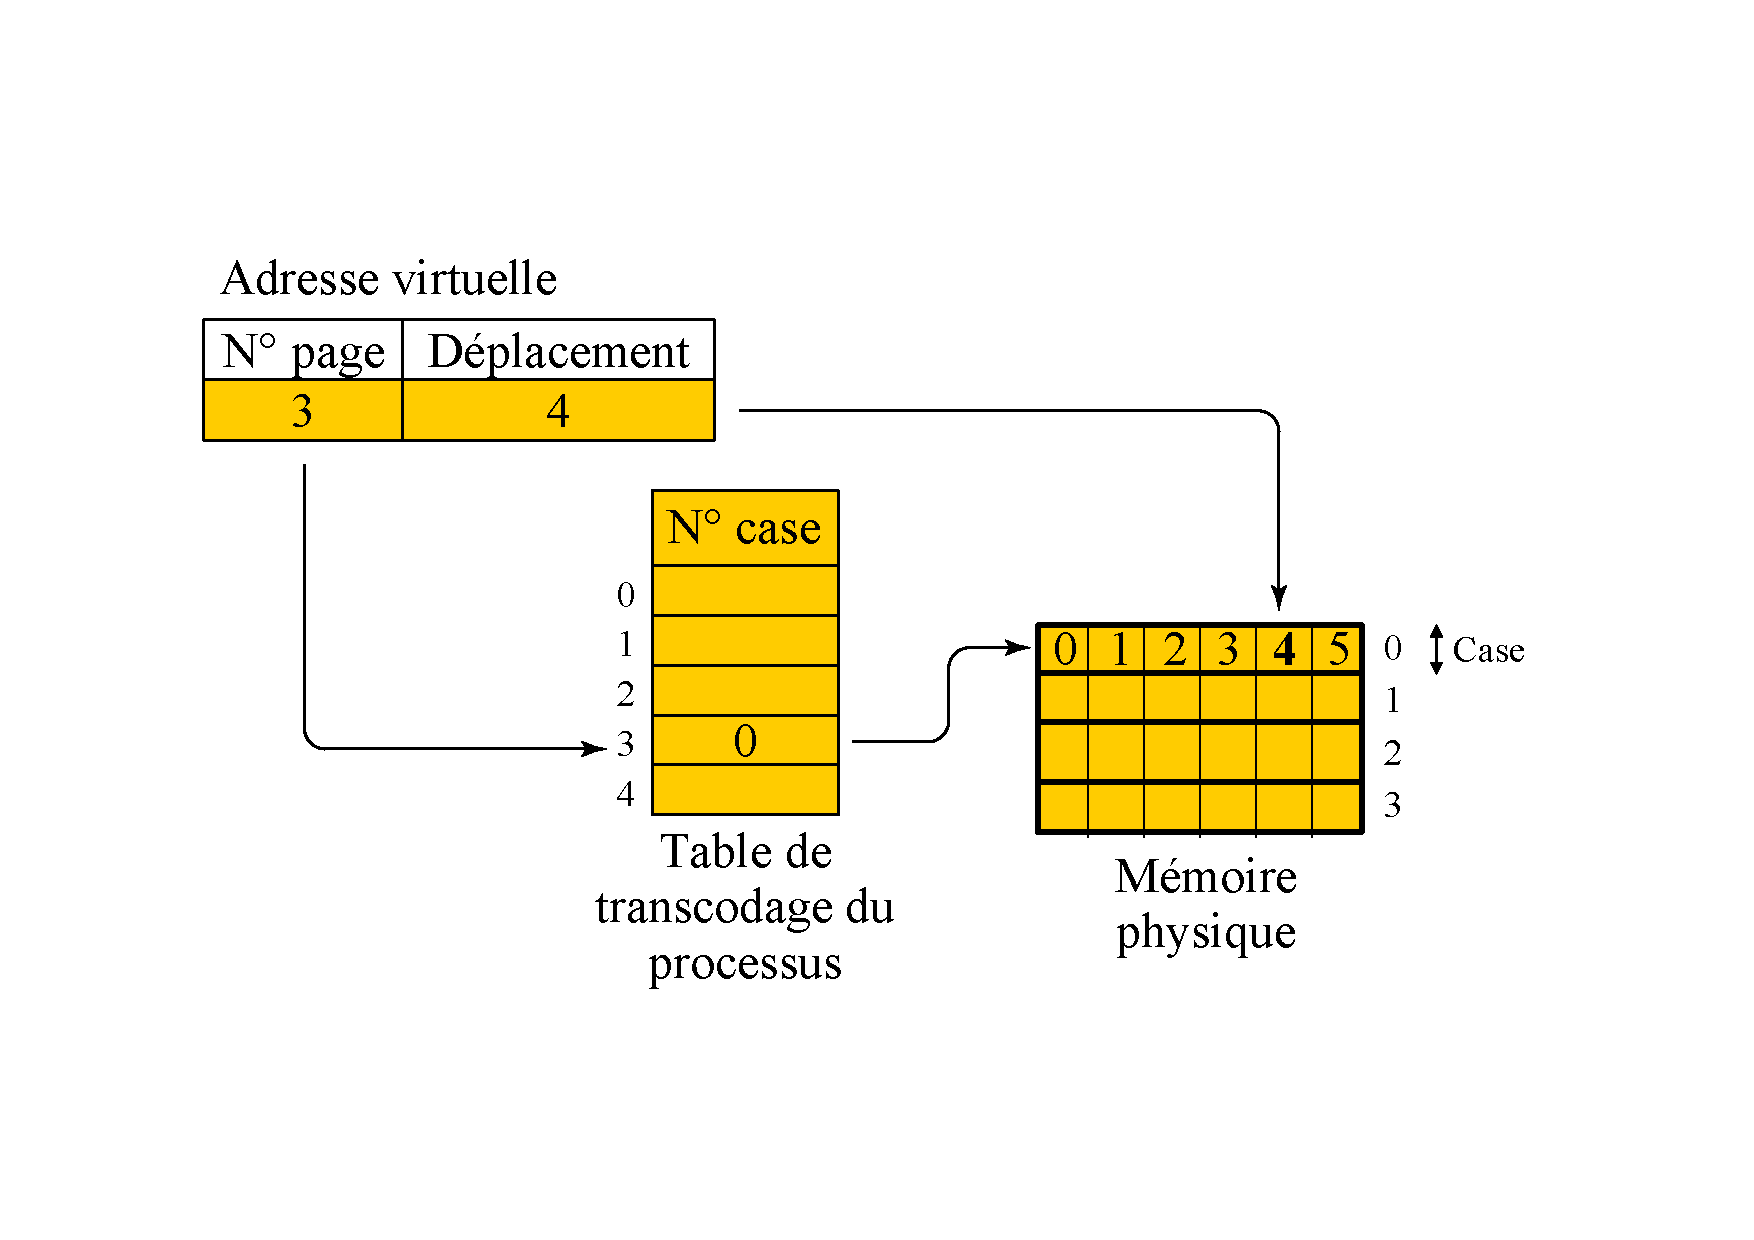
\includegraphics[width=\textwidth]{../illustration/memoire_paginee_tab_transcodage.pdf}
\end{frame}


\begin{frame}
\frametitle{Exemple de pagination}
\begin{itemize}
\item Architecture x86 :
\begin{itemize}
\item Taille des pages :
4Ko, soit une taille de 4096 octets
\end{itemize}
\item Adresses 32 bits composées de :
\begin{itemize}
\item Déplacement (offset) sur 12 bits ($2^{12}$ = 4096)
\item Numéro de page codé sur 20 bits
\end{itemize}
\item Il y a donc $2^{20}$, soit 1 048 576 pages adressables au maximum (4 Go)
\end{itemize}
\end{frame}

\begin{frame}
\frametitle{}
\begin{columns}
\column{0.5\textwidth}
\begin{block}{Avantages}
\begin{itemize}
\item Permet l'allocation / libération dynamique de mémoire
\item Supprime les problèmes liés à la fragmentation externe
\item Protection mémoire entre processus
\item Partage de données possible
\end{itemize}
\end{block}
\column{0.5\textwidth}
\begin{block}{Inconvénients}
\begin{itemize}
\item Fragmentation interne (dernière page)
\item Pas de vue générale des espaces mémoire alloués aux processus
\item Notion de page souvent trop fine (protection, partage de mémoire… )
\item Occupation mémoire des tables des pages
\item La table des pages ne peut être fractionnée
\end{itemize}
\end{block}
\end{columns}
\end{frame}



\begin{frame}
\frametitle{La segmentation paginée}
Principe :
\begin{itemize}
\item Combinaison pagination et segmentation
\begin{itemize}
\item Regroupement des pages en segments
\item Segment composé de pages
\end{itemize}
\item Partage de pages possible entre segments
\begin{itemize}
\item Limite le fractionnement interne
\end{itemize}
\item Permet de gérer des segments non contigus
\begin{itemize}
\item Table des segments
\item Une table des pages pour chaque segment
\end{itemize}
\end{itemize}
\end{frame}



\begin{frame}
\frametitle{La segmentation paginée - exemple}
\begin{columns}
\column{.5\textwidth}
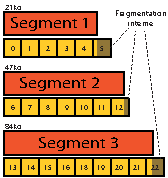
\includegraphics[height=0.8\textheight]{../illustration/memoire_segment_paginee_exemple.pdf}
\column{.5\textwidth}
\begin{table}[htdp]
\caption{Table des segments}
\begin{center}
\begin{tabular}{c|c}
Etendue & Déplacement \\
\hline
21ko & 0 \\ 
47ko & 0 \\
84ko & 0 \\
\end{tabular}
\end{center}
\end{table}
\end{columns}
\end{frame}

\begin{frame}
\frametitle{La segmentation paginée - partage de pages}
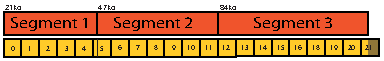
\includegraphics[width=\textwidth]{../illustration/memoire_segment_paginee_exemple_partage.pdf}

\begin{table}[htdp]
\caption{Table des segments}
\begin{center}
\begin{tabular}{c|c}
Etendue & Déplacement \\
\hline
21ko & 0 \\ 
47ko & 1 \\
84ko & 0 \\
\end{tabular}
\end{center}
\end{table}
\end{frame}

\begin{frame}
\frametitle{La segmentation paginée}
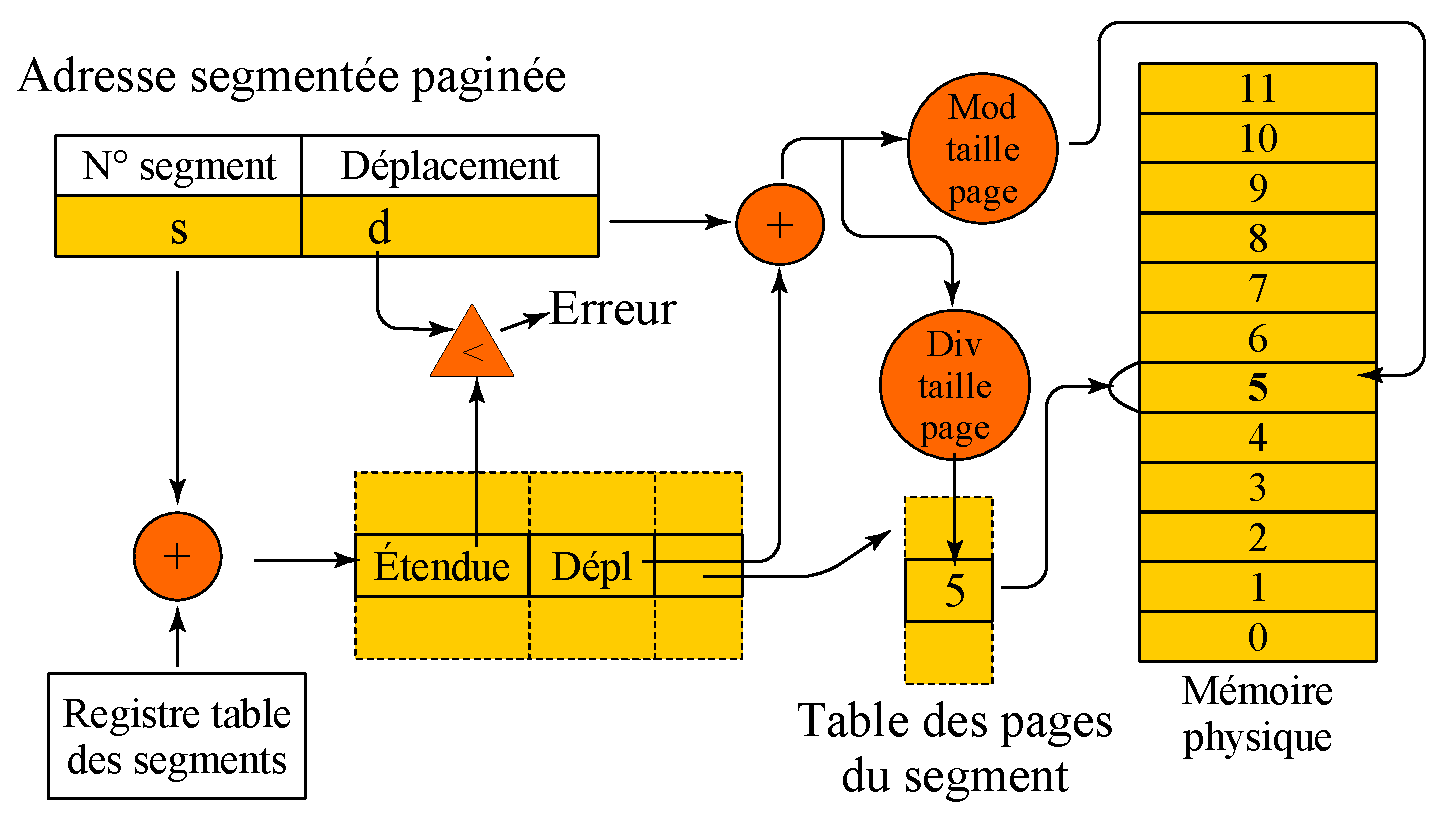
\includegraphics[width=\textwidth]{../illustration/memoire_segment_paginee_calcul.pdf}
\end{frame}


\begin{frame}
\frametitle{La segmentation paginée}
\begin{itemize}
\item Manipulation d'ensembles de mémoire plus grands
\begin{itemize}
\item Protection des segments et non de chaque page du segment
\item Partage de segments
\end{itemize}
\item Permet de limiter le fractionnement interne
\begin{itemize}
\item Uniquement dernière page de l'espace d'un processus et non sur chaque segment
\end{itemize}
\end{itemize}
\end{frame}


\begin{frame}
\frametitle{Recouvrement de programmes}
Double problématique :
\begin{itemize}
\item Exécuter un processus plus volumineux que la mémoire disponible
\item Exécuter simultanément un ensemble de processus quand la mémoire principale ne peut pas les contenir tous
\end{itemize}
\end{frame}

\begin{frame}
\frametitle{Notion de recouvrement}
\begin{itemize}
\item Stratégie de recouvrement (\textit{overlay})
\item Principe :
\begin{itemize}
\item Chargement en mémoire des seuls éléments nécessaires à l'exécution immédiate
\end{itemize}
\item Solutions possibles :
\begin{itemize}
\item Découpage en modules chargés dynamiquement
\item Va et vient - permutation de processus
\end{itemize}
\end{itemize}
\end{frame}

\begin{frame}
\frametitle{Recouvrement par découpage en module}
\begin{itemize}
\item Ne conserver en mémoire que les informations nécessaires
\item Pris en charge par le programmeur
\begin{itemize}
\item Seuls les modules et données nécessaires sont explicitement chargés en mémoire
\end{itemize}
\item Fastidieux :
\begin{itemize}
\item Découpage programme (programmation)
\item Lié configuration/charge système (portabilité)
\item Manque de souplesse
\end{itemize}
\end{itemize}
\end{frame}

\begin{frame}
\frametitle{Chargement dynamique}
\begin{itemize}
\item Programmes et données doivent résider en mémoire pour permettre l'exécution
\begin{itemize}
\item Au moins la prochaine instruction à exécuter
\end{itemize}
\item Chargement dynamique (run time) :
\begin{itemize}
\item Découpage des programmes en routines
\item Chargement des routines au fur et à mesure des appels
\item Routines non utilisées stockées sur disque
\item Chargeur - éditeur de lien dynamique
\end{itemize}
\end{itemize}
\end{frame}

\begin{frame}
\frametitle{Chargement dynamique}
\begin{itemize}
\item Avantages :
\begin{itemize}
\item Les routines non utilisées ne sont pas chargées en mémoire
\item Possibilité de manipuler un ensemble de programmes et de données plus volumineux que la mémoire physique disponible
\end{itemize}
\item Découpage défini par le programmeur
\begin{itemize}
\item Contraintes physiques : taille mémoire...
\end{itemize}
\item Recouvrement géré par le système
\end{itemize}
\end{frame}


\begin{frame}
\frametitle{Stratégie de recouvrement : Exemple}
\begin{itemize}
\item Assembleur en deux phases :
\begin{itemize}
\item Phase 1 : Construction table des symboles
\item Phase 2 : Génération du code
\end{itemize}
\item Tailles mémoire :
\begin{itemize}
\item Table des symboles : 20 Ko
\item Routines communes : 50 Ko
\item Phase 1 : 120 Ko, Phase 2 : 60 Ko
\end{itemize}
\item Mémoire système : 200 Ko (et non 250)
\end{itemize}
\end{frame}


\begin{frame}
\frametitle{Stratégie de recouvrement : Exemple}
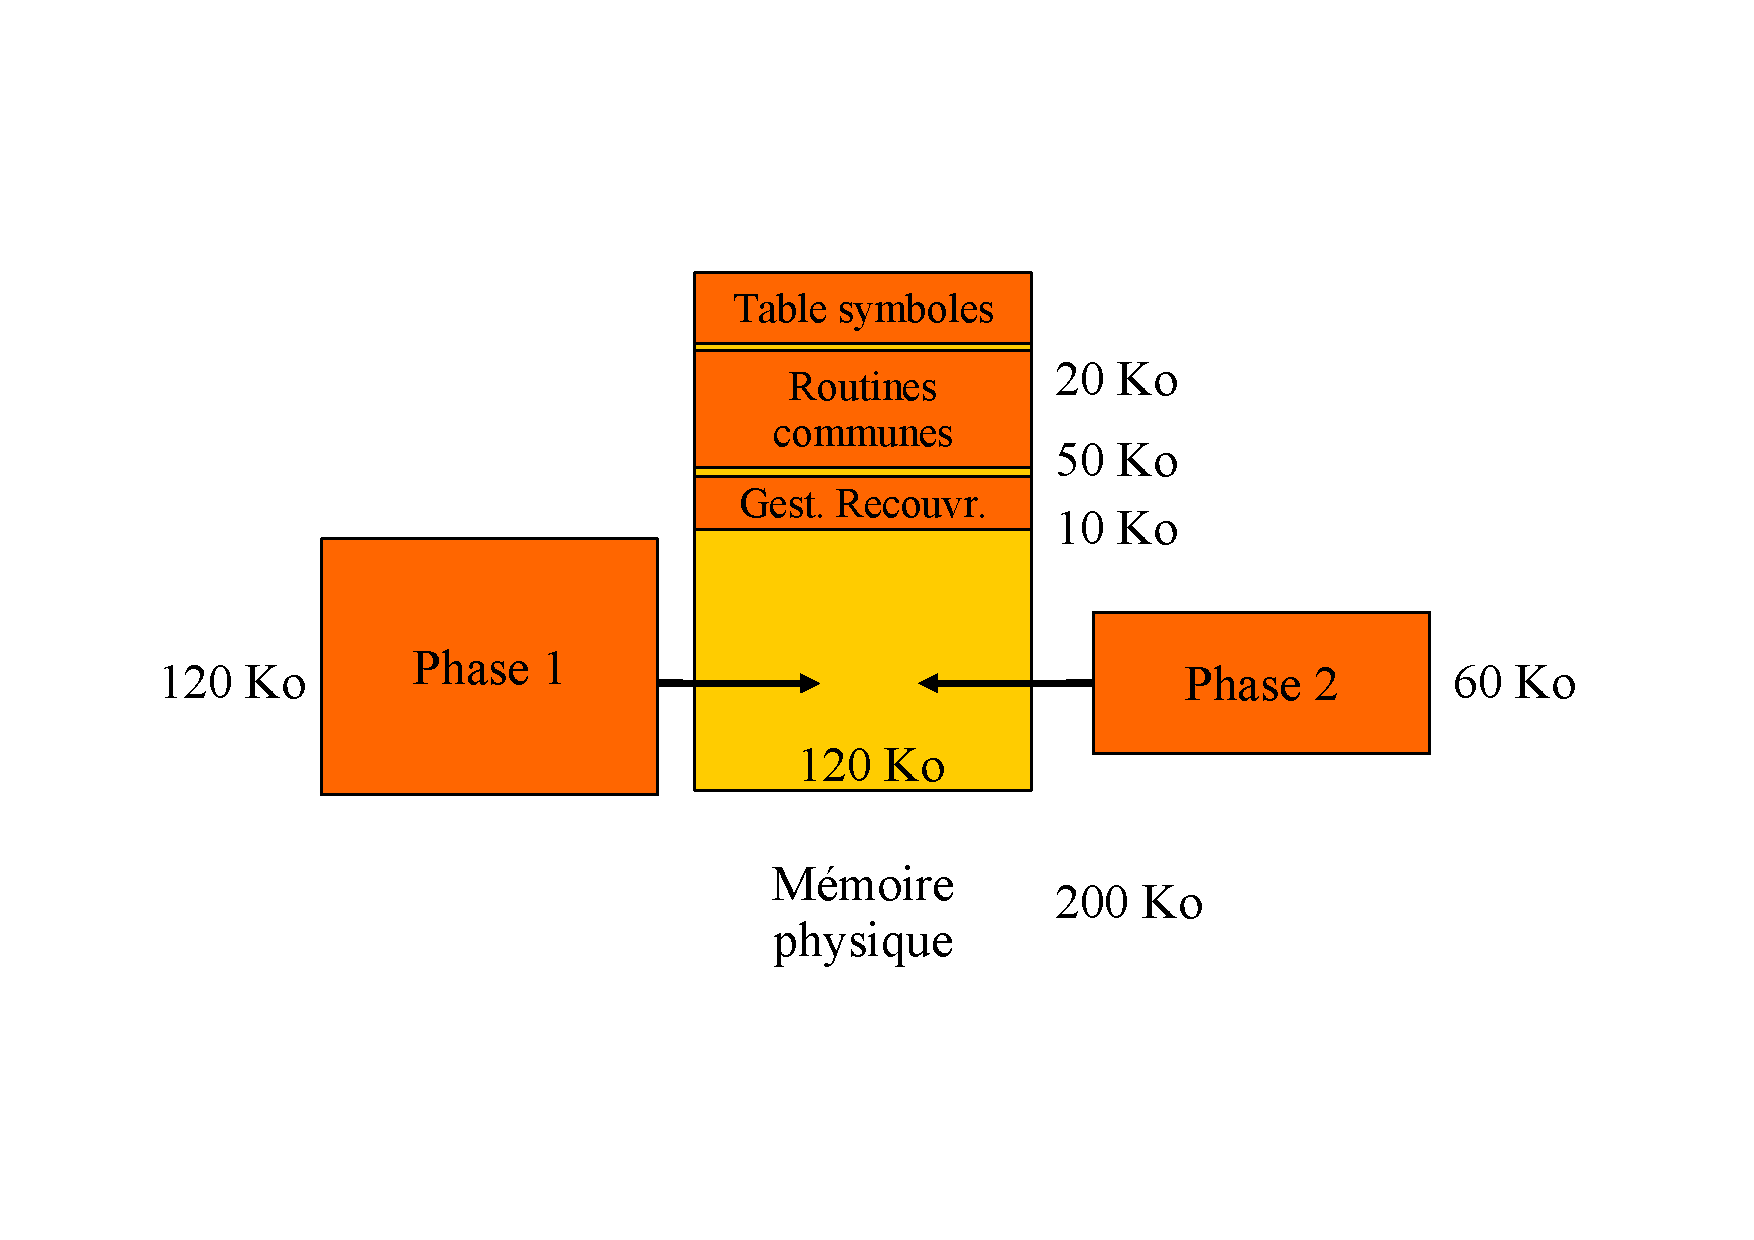
\includegraphics[width=\textwidth]{../illustration/recouvrement_exemple.pdf}
\end{frame}


\begin{frame}
\frametitle{Liaison dynamique et bibliothèques partagées}
\begin{itemize}
\item Édition de liens statique : 
\begin{itemize}
\item Liaison de toutes les bibliothèques dans le fichier exécutable $\rightarrow$ exécutable monolithique
\end{itemize}
\item Édition de liens dynamique :
\begin{itemize}
\item Liaison et chargement reportés au plus tard
\begin{itemize}
\item Au moment de l'exécution
\end{itemize}
\item Évite duplication des bibliothèques
\begin{itemize}
\item Bibliothèques partagées
\end{itemize}
\item Ne charge que le strict nécessaire
\end{itemize}
\end{itemize}
\end{frame}


\begin{frame}
\frametitle{Liaison dynamique et bibliothèques partagées}
\begin{itemize}
\item Stub :
\begin{itemize}
\item Élément de remplacement (pointeur)
\item Inséré dans l'image, à la place d'une référence à la bibliothèque (indication de la version)
\item Vérifie la présence de la routine utilisée en mémoire et la charge si besoin
\end{itemize}
\item Assistance de la part du système
\begin{itemize}
\item Permet à plusieurs processus d'accéder aux mêmes bibliothèques partagées
\end{itemize}
\end{itemize}
\end{frame}

\begin{frame}
\frametitle{Va et vient - permutation}
\begin{itemize}
\item Stratégie de recouvrement
\item Tous les processus ne peuvent pas tenir simultanément en mémoire
\item Déplacement temporaire de certains sur une mémoire provisoire
\begin{itemize}
\item Partie réservée du disque (\textit{swap area} ou \textit{backing store})
\item Gestion de la zone de va et vient comparable à celle de la mémoire principale
\item Algorithme de rotation du cache
\end{itemize}
\end{itemize}
\end{frame}


\begin{frame}
\frametitle{Va et vient - permutation}
\begin{itemize}
\item Swap out :
\begin{itemize}
\item Déchargement de la mémoire principale
\item Déplacement d'un processus de la mémoire principale vers la mémoire secondaire
\end{itemize}
\item Swap in :
\begin{itemize}
\item Chargement de la mémoire principale
\item Déplacement d'un processus de la mémoire secondaire vers la mémoire principale
\end{itemize}
\end{itemize}
\end{frame}


\begin{frame}
\frametitle{Va et vient - permutation}
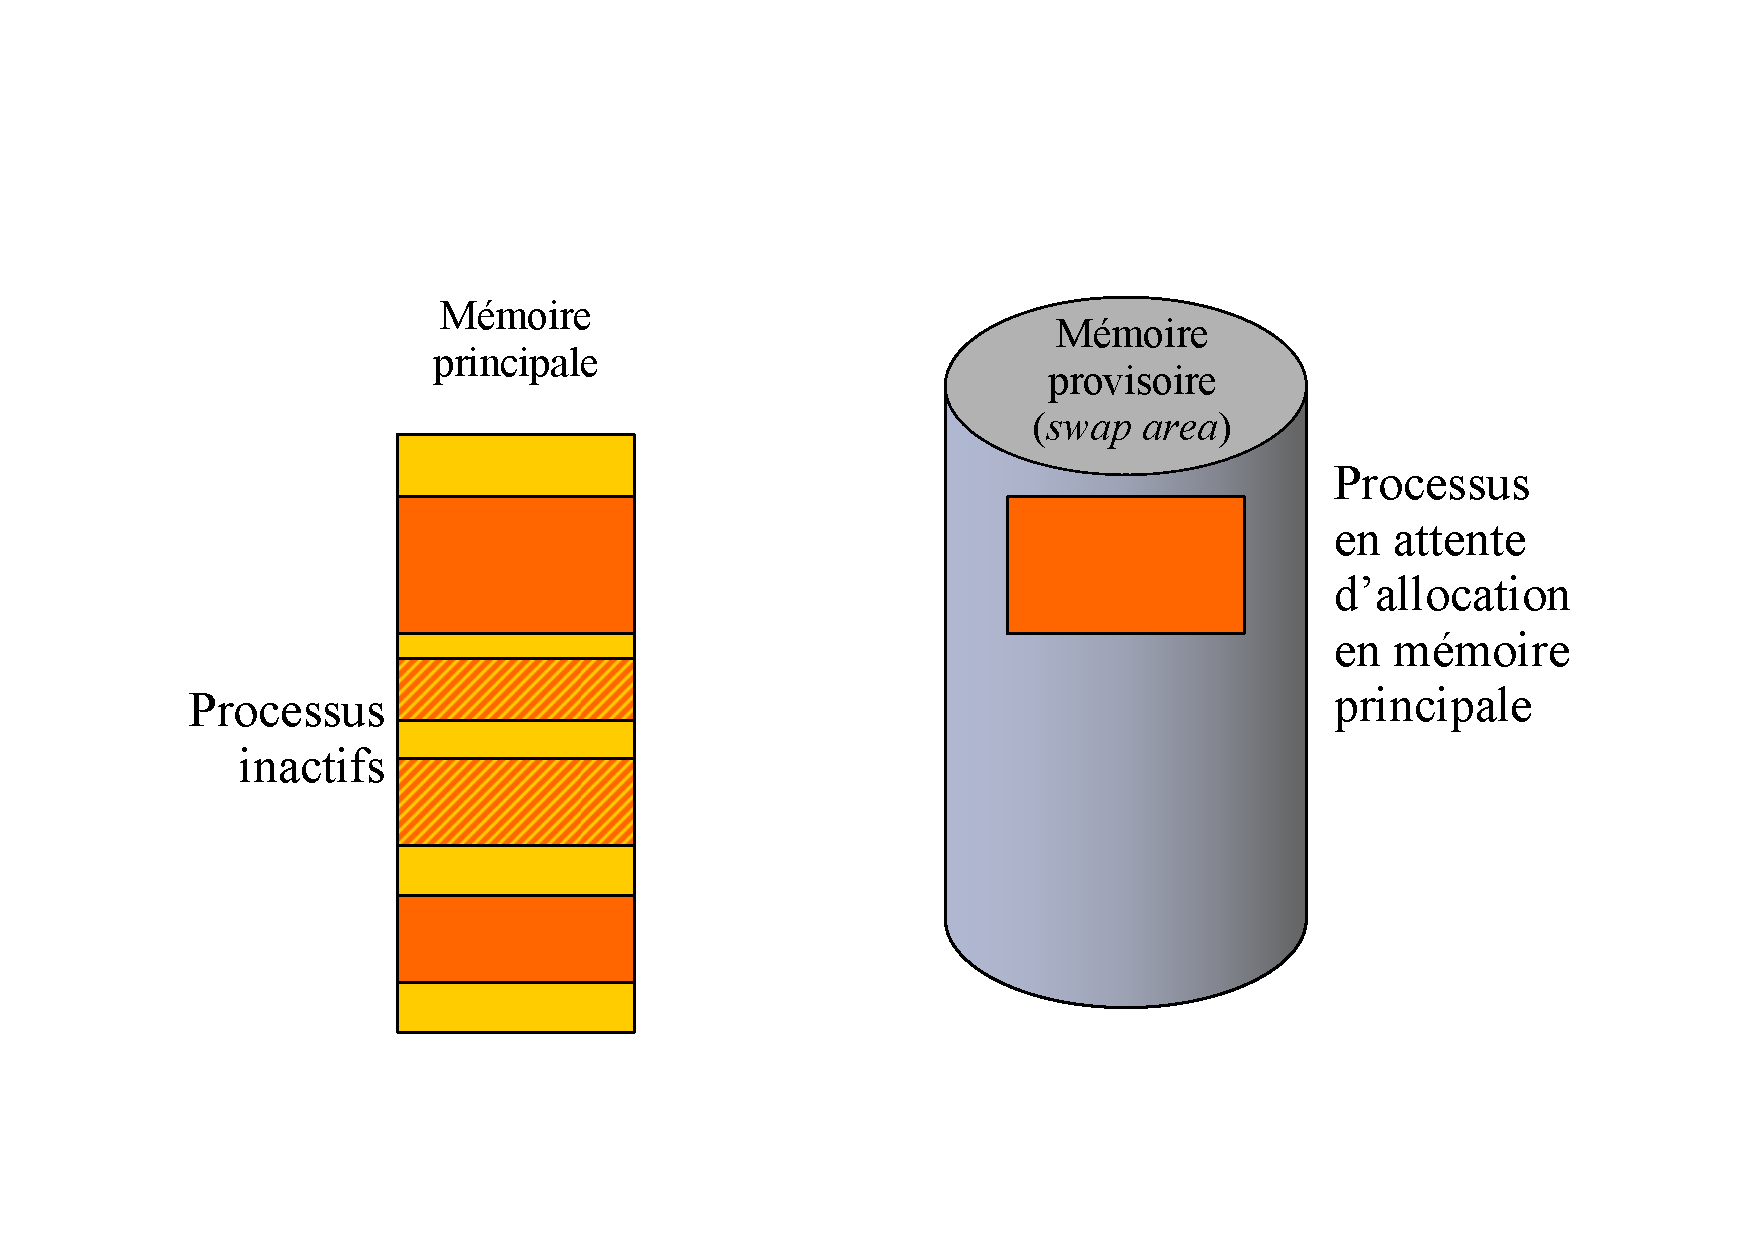
\includegraphics[width=\textwidth]{../illustration/permut_swap_exemple.pdf}
\end{frame}


\begin{frame}
\frametitle{Va et vient - permutation}
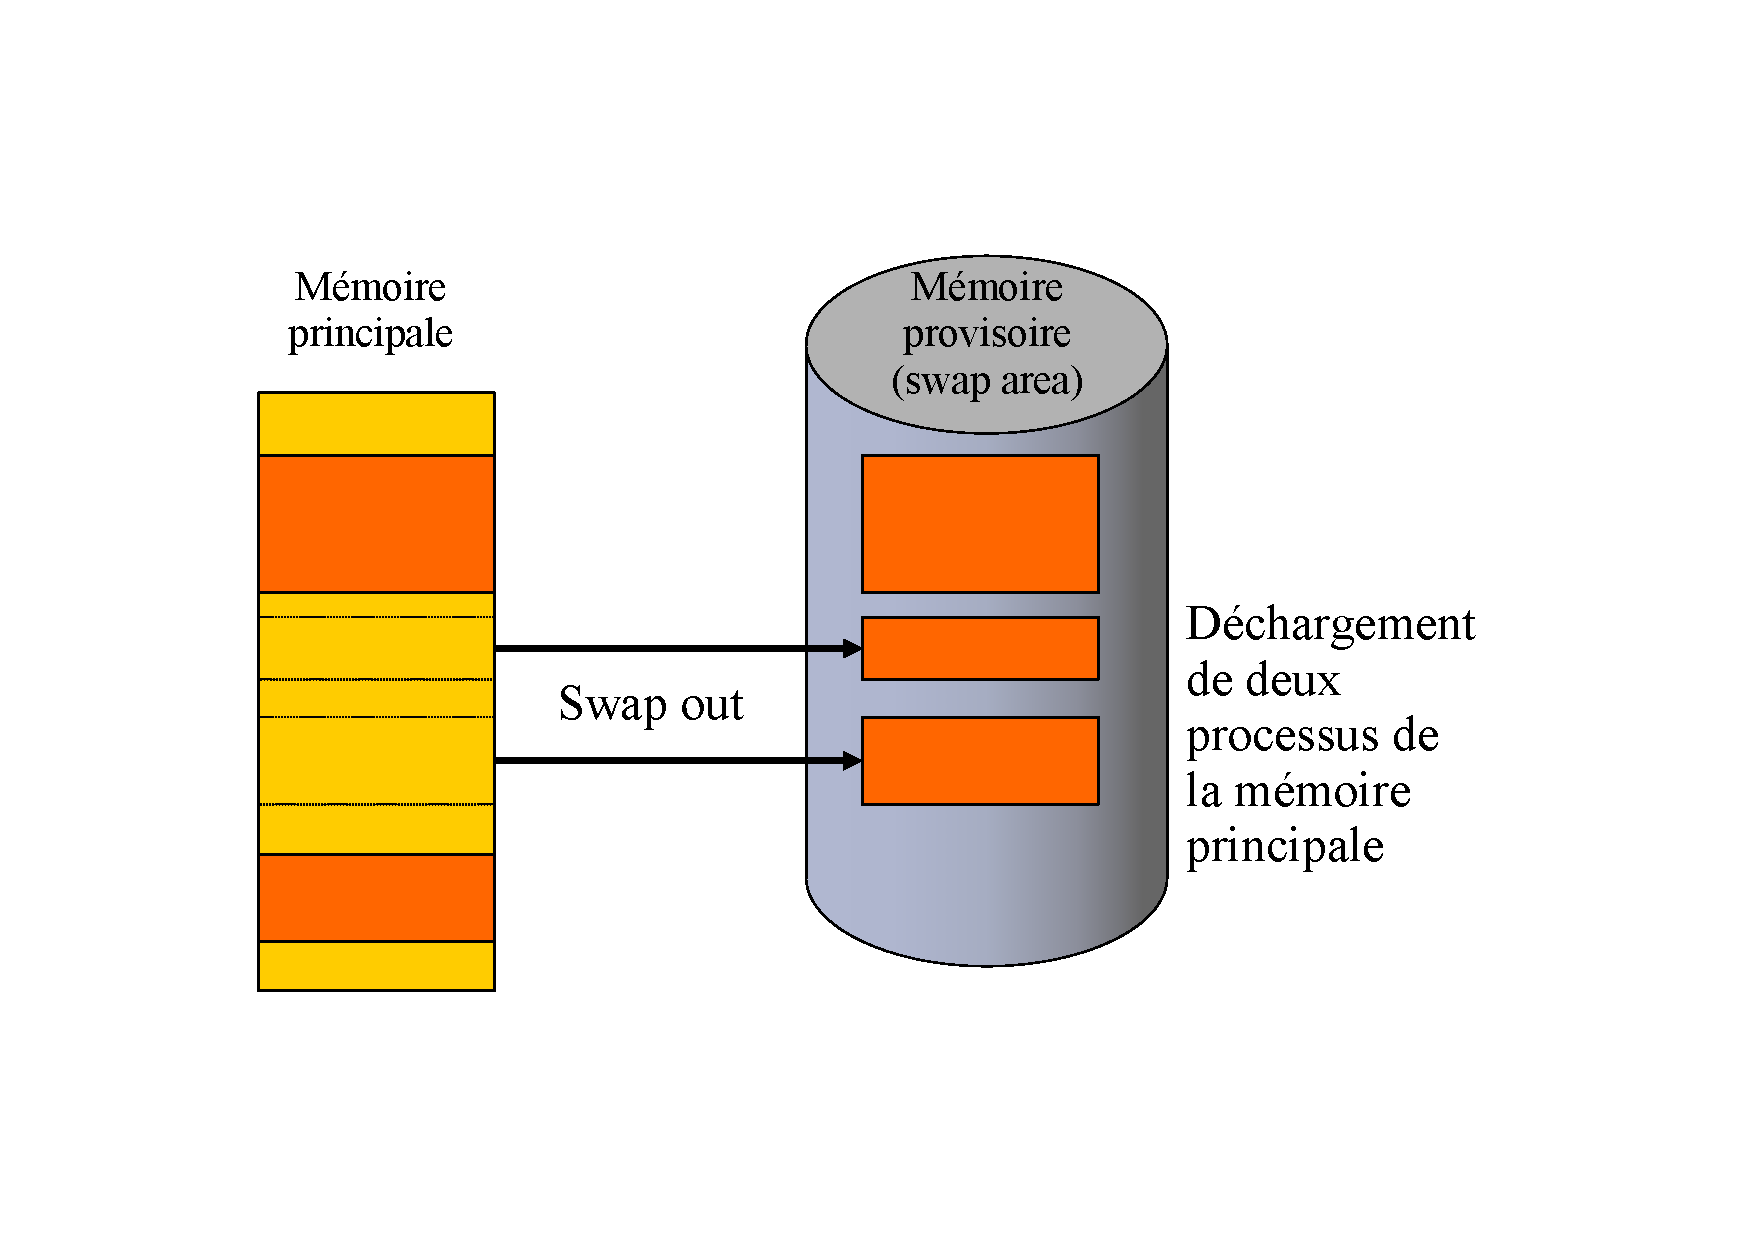
\includegraphics[width=.9\textwidth]{../illustration/permut_swap_exemple2.pdf}
\end{frame}


\begin{frame}
\frametitle{Va et vient - permutation}
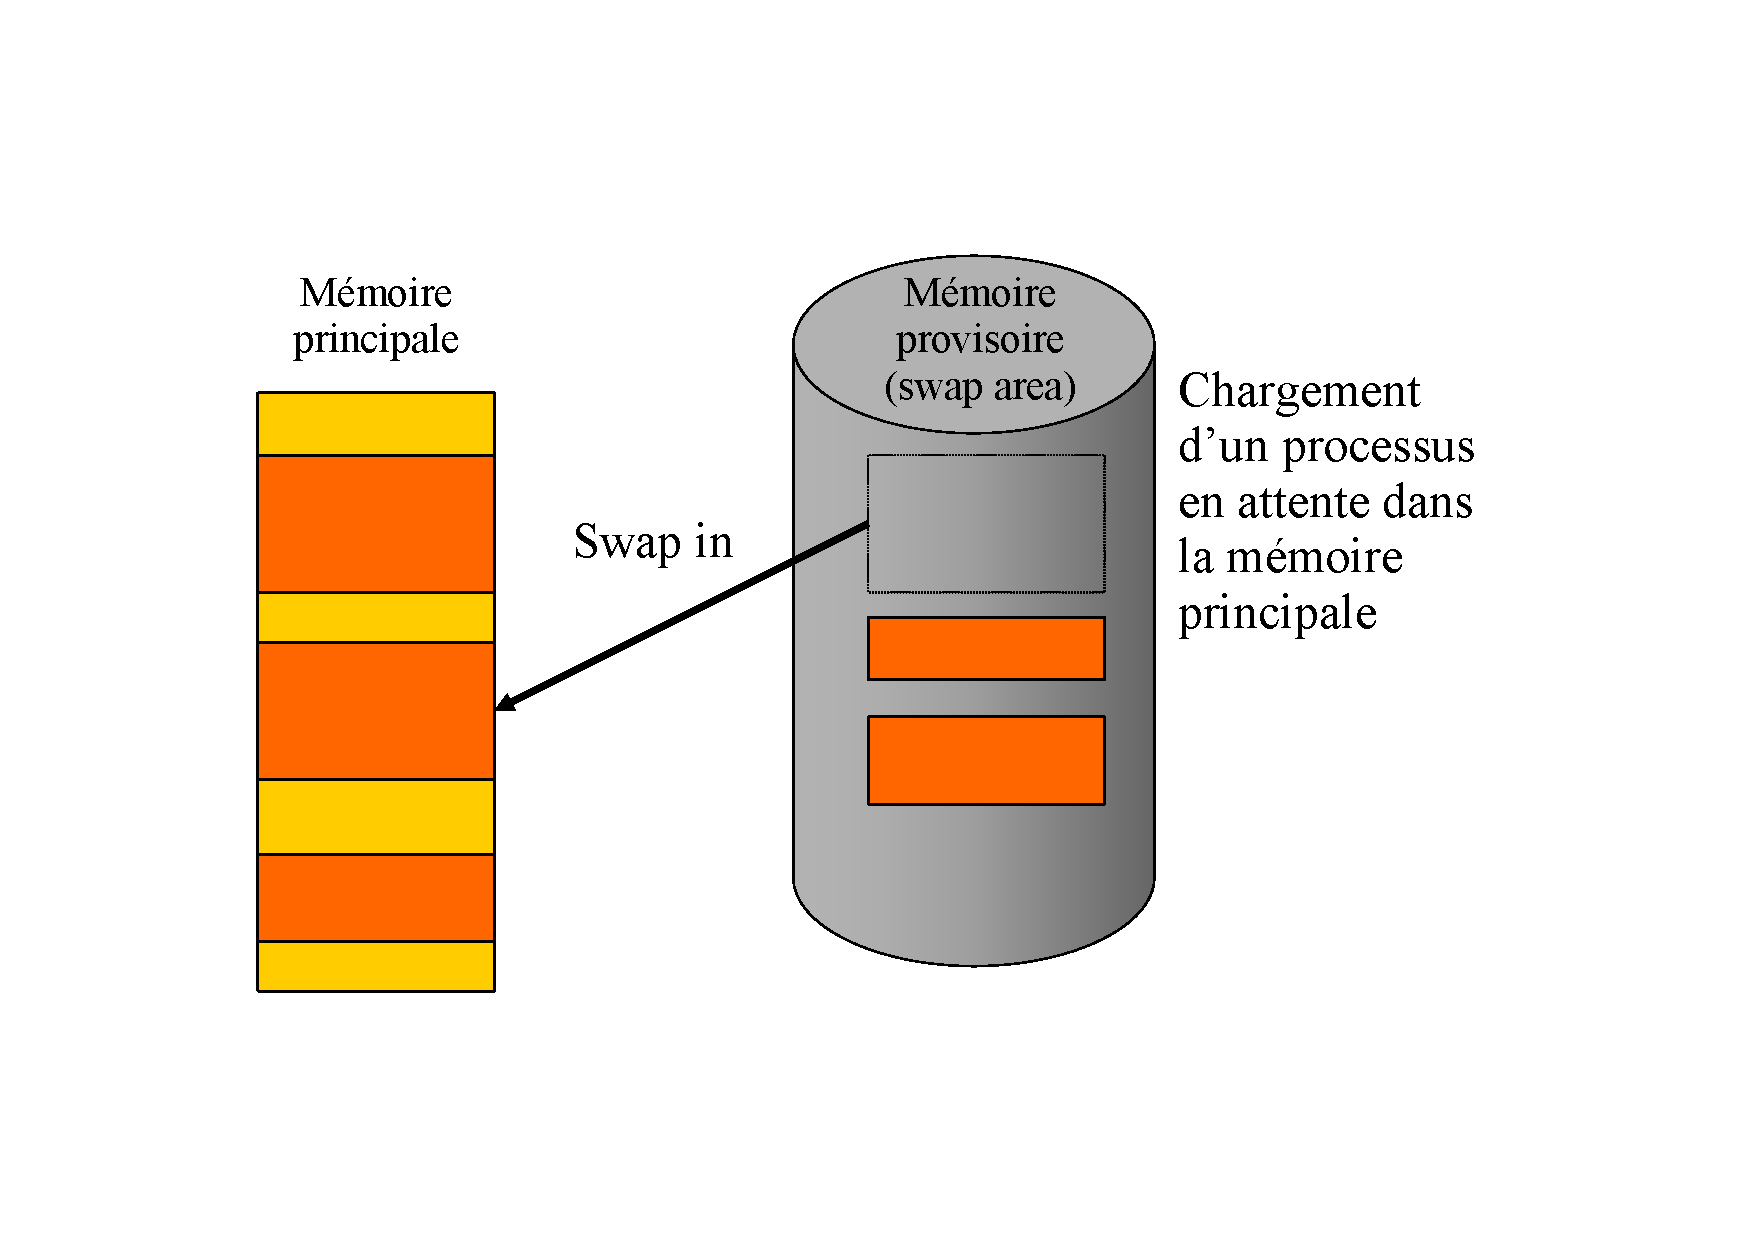
\includegraphics[width=.9\textwidth]{../illustration/permut_swap_exemple3.pdf}
\end{frame}


\begin{frame}
\frametitle{Va et vient - permutation}
\begin{itemize}
\item Exemple :
\begin{itemize}
\item Programme 125 KO
\item Disque temps moyen d'accès : 10 ms
\item Débit : 250 KO/sec
\item 10 ms + 500 ms
\begin{itemize}
\item 510 ms pour le swap in
\item A ajouter au temps d'accès mémoire (minime)
\end{itemize}
\end{itemize}
\item Intéressant si l'exécution est nettement plus longue que le temps de l'échange
\end{itemize}
\end{frame}


\begin{frame}
\frametitle{Va et vient - permutation}
\begin{itemize}
\item Permet de pallier au manque de mémoire nécessaire à plusieurs processus
\item Augmente le délai de commutation de contexte
\begin{itemize}
\item Favorise de déroulement des processus et non l'utilisation du processeur
\end{itemize}
\item Ne permet pas d'exécuter des programmes de taille supérieure à celle de la mémoire physique
\end{itemize}
\end{frame}



%-----------------------------------------------
\subsection{Mémoire virtuelle}
%-----------------------------------------------
\begin{frame}
\frametitle{Pourquoi une mémoire virtuelle ?}
Conséquences du chargement de la totalité des programmes en mémoire centrale :
\begin{itemize}
\item Sous-utilisation de la mémoire :
\begin{itemize}
\item La totalité du programme est rarement utilisée en même temps et en permanence
\end{itemize}
\item Impossibilité d'exécuter certains programmes :
\begin{itemize}
\item Programmes plus volumineux que la mémoire centrale. 
\end{itemize}
\end{itemize}
\end{frame}


\begin{frame}
\frametitle{Pourquoi une mémoire virtuelle ?}
\begin{itemize}
\item La mémoire disponible est rarement suffisante
\begin{itemize}
\item Plus coûteuse que la mémoire secondaire
\item Programmes exigeants souvent plus de mémoire que la quantité disponible
\end{itemize}
\item Idée :
\begin{itemize}
\item Utiliser la mémoire secondaire comme une extension de la mémoire principale
\item Faire croire au programmeur qu'il dispose d'une plus grande quantité de mémoire
\end{itemize}
\end{itemize}
\end{frame}


\begin{frame}
\frametitle{Mémoire virtuelle}
\begin{itemize}
\item Technique permettant l'exécution d'un programme sans qu'il se trouve en totalité en mémoire centrale
\item Libération du programmeur des préoccupations du découpage des programmes pour « tenir » en mémoire
\item Mémoire virtuelle
\begin{itemize}
\item Mémoire principale + partie mémoire secondaire
\end{itemize}
\end{itemize}
\end{frame}


\begin{frame}
\frametitle{Mémoire virtuelle}
\begin{itemize}
\item Services apportés par le système
\item Avantages :
\begin{itemize}
\item Portabilité, moindre dépendance des programmes par rapport :
\begin{itemize}
\item à la taille de la mémoire effectivement utilisable
\item à la charge du système
\end{itemize}
\item Meilleurs taux d'utilisation du processeur
\begin{itemize}
\item Permet d'augmenter le taux de multiprogrammation
\end{itemize}
\end{itemize}
\end{itemize}
\end{frame}

\begin{frame}
\frametitle{Mémoire virtuelle : Définition}
\begin{itemize}
\item Mémoire physique
\begin{itemize}
\item Ensemble des emplacements RAM physiquement présents dans l'ordinateur
\end{itemize}
\item Mémoire virtuelle
\begin{itemize}
\item Support de l'ensemble des informations potentiellement accessibles
\item Ensemble des emplacements dont l'adresse peut être engendrée par le processeur
\item Toutes les adresses utilisées dans les instructions sont virtuelles
\end{itemize}
\end{itemize}
\end{frame}


\begin{frame}
\frametitle{Implémentation de la mémoire virtuelle}
\begin{itemize}
\item Pagination à la demande:
\begin{itemize}
\item Pagination mémoire principale et secondaire
\item Conserve en mémoire principale les seuls blocs nécessaires aux programmes en cours d'exécution
\end{itemize}
\item Segmentation paginée :
\begin{itemize}
\item Segments répartis en pages
\end{itemize}
\item Segmentation à la demande :
\begin{itemize}
\item Algorithmes complexes
\end{itemize}
\end{itemize}
\end{frame}


\begin{frame}
\frametitle{Mémoire virtuelle paginée}
\begin{itemize}
\item Découpage en \textbf{pages} de taille fixe :
\begin{itemize}
\item Programmes et données en mémoire virtuelle
\item Processus = ensemble de pages individuelles
\end{itemize}
\item Découpage en \textbf{cases} de taille fixe :
\begin{itemize}
\item De la mémoire principale
\item De la mémoire secondaire
\end{itemize}
\item Stockage pages virtuelles dans les cases :
\begin{itemize}
\item En mémoire secondaire (systématiquement)
\item En mémoire principale (pour utilisation)
\end{itemize}
\end{itemize}
\end{frame}


\begin{frame}
\frametitle{Type de pagination}
\begin{itemize}
\item Pagination par \textbf{permutation} :
\begin{itemize}
\item Déplacement de toutes les pages d'un processus entre la mémoire principale et la mémoire secondaire
\end{itemize}
\item Pagination par \textbf{échangeur paresseux} (pagination à la demande) :
\begin{itemize}
\item Ne transfère en mémoire principale que les pages indispensables
\begin{itemize}
\item Celles qui vont être utilisées pour la prochaine instruction
\end{itemize}
\end{itemize}
\end{itemize}
\end{frame}


\begin{frame}
\frametitle{Corres. adr. virtuelle  $\Leftrightarrow$  physique}
\begin{itemize}
\item Utilisation d'une fonction topographique associant une page virtuelle à une page physique 
\begin{itemize}
\item Table des pages virtuelles
\end{itemize}
\item Programmes ré-entrants ou partage de données :
\begin{itemize}
\item Code réentrant, non variant ou «code pur» n'est pas modifié au cours de l'exécution : il peut être partagé
\item Partage de pages entre plusieurs processus
\end{itemize}
\end{itemize}
\end{frame}


\begin{frame}
\frametitle{Table des pages virtuelles}
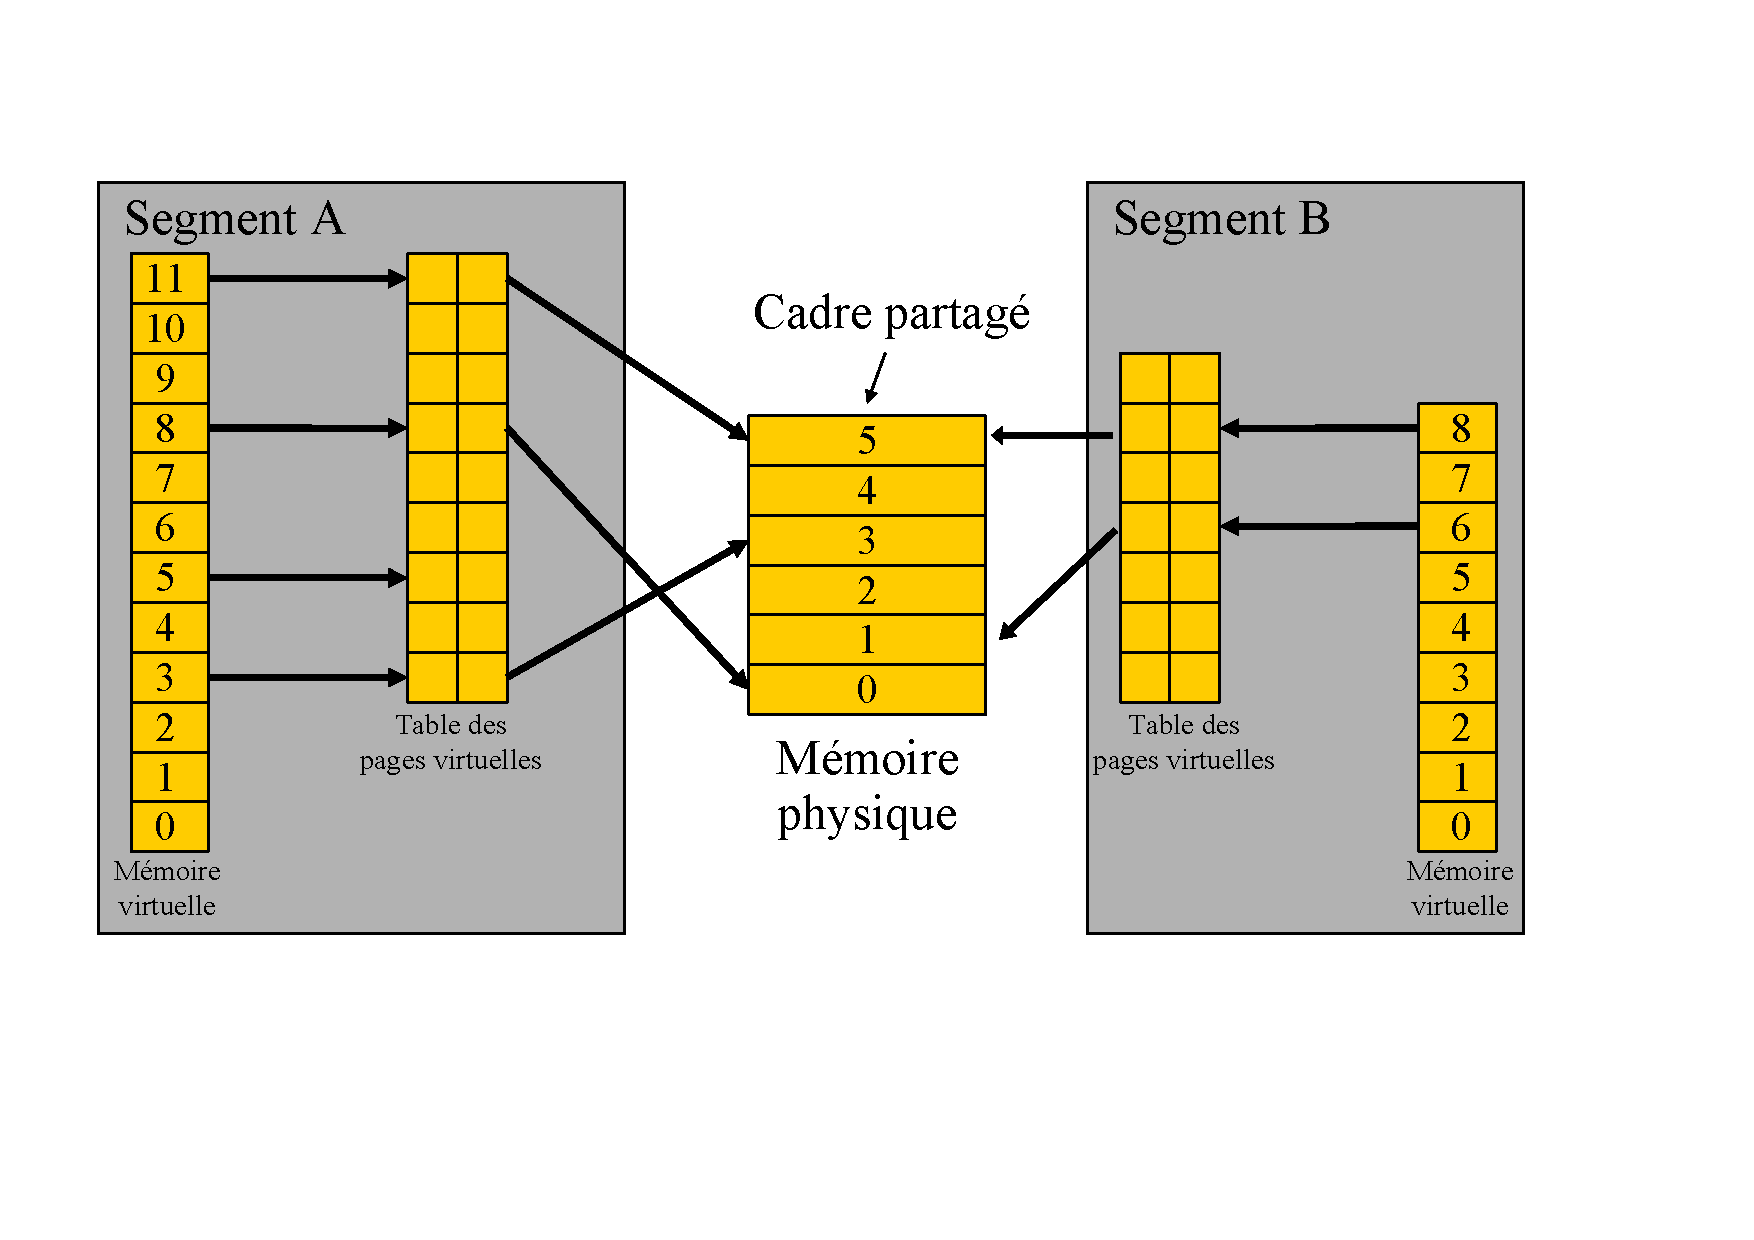
\includegraphics[width=.9\textwidth]{../illustration/table_pages_virtuelles.pdf}
\end{frame}

\begin{frame}
\frametitle{Contenu de la table des pages}
\begin{itemize}
\item Champs :
\begin{itemize}
\item \textbf{Présent} : Page en mémoire physique ?
\item \textbf{Modifié} : Page modifiée ?
\item \textbf{Protection} : Droits d'accès à la page
\item \textbf{Num. page physique} : Case mémoire correspondante
\end{itemize}
\end{itemize}
\begin{block}{Exemple}
\begin{tabular}{l|l|l|l}
Présent & Modifié & Protection & N de page physique \\
\hline
Oui & Non & R & 254 \\
Oui & Non & RW & 587 \\
Non & Non & RW & \\
\end{tabular}
\end{block}
\end{frame}

\begin{frame}
\frametitle{Support matériel de la pagination}
\begin{itemize}
\item <1>\textbf{Registres dédiés} :
\begin{itemize}
\item Stockage de la table des pages virtuelles
\item Rapide, mais capacité limitée (exemple : 256 entrées)
\end{itemize}
\item <2>\textbf{Registre pointant vers la table des pages} :
\begin{itemize}
\item \textbf{PTBR} : Page Table Base Register
\item Stockage de la table des pages virtuelles en mémoire centrale
\item Deux accès mémoire
\end{itemize}
\item <3>\textbf{Registres associatifs} :
\begin{itemize}
\item \textbf{TLB} : Translation Look-aside Buffer
\item Mise en cache des adresses des pages les plus utilisées
\item Propre à chaque processus - fait partie du PSW
\end{itemize}
\end{itemize}
\end{frame}


\begin{frame}
\frametitle{Le problème de la taille de la TPV}
\begin{itemize}
\item Pour être utilisée, la TPV doit être placée en mémoire physique.
\begin{itemize}
\item Par exemple :
\begin{itemize}
\item $2^{20}$ pages virtuelles,
\item Taille TPV = $2^{20} * $ taille d'une entrée,
\item = 10 Mo si une entrée tient sur 10 octets.
\item Encombrement mémoire physique
\end{itemize}
\end{itemize}
\item Solution :
\begin{itemize}
\item Paginer la TPV
\end{itemize}
\end{itemize}
\end{frame}

\begin{frame}
\frametitle{Pagination à deux niveaux}
\begin{itemize}
\item La mémoire virtuelle est divisée en \textbf{hyperpages} qui sont elles-mêmes divisées en \textbf{pages}
\item Adresse virtuelle :
\begin{itemize}
\item Numéro d'hyperpage + numéro de page + déplacement
\end{itemize}
\item L'accès à la mémoire est plus lent
\begin{itemize}
\item Un accès mémoire supplémentaire
\end{itemize}
\item La mémoire virtuelle est toujours linéaire
\end{itemize}
\end{frame}


\begin{frame}
\frametitle{Pagination à deux niveaux}
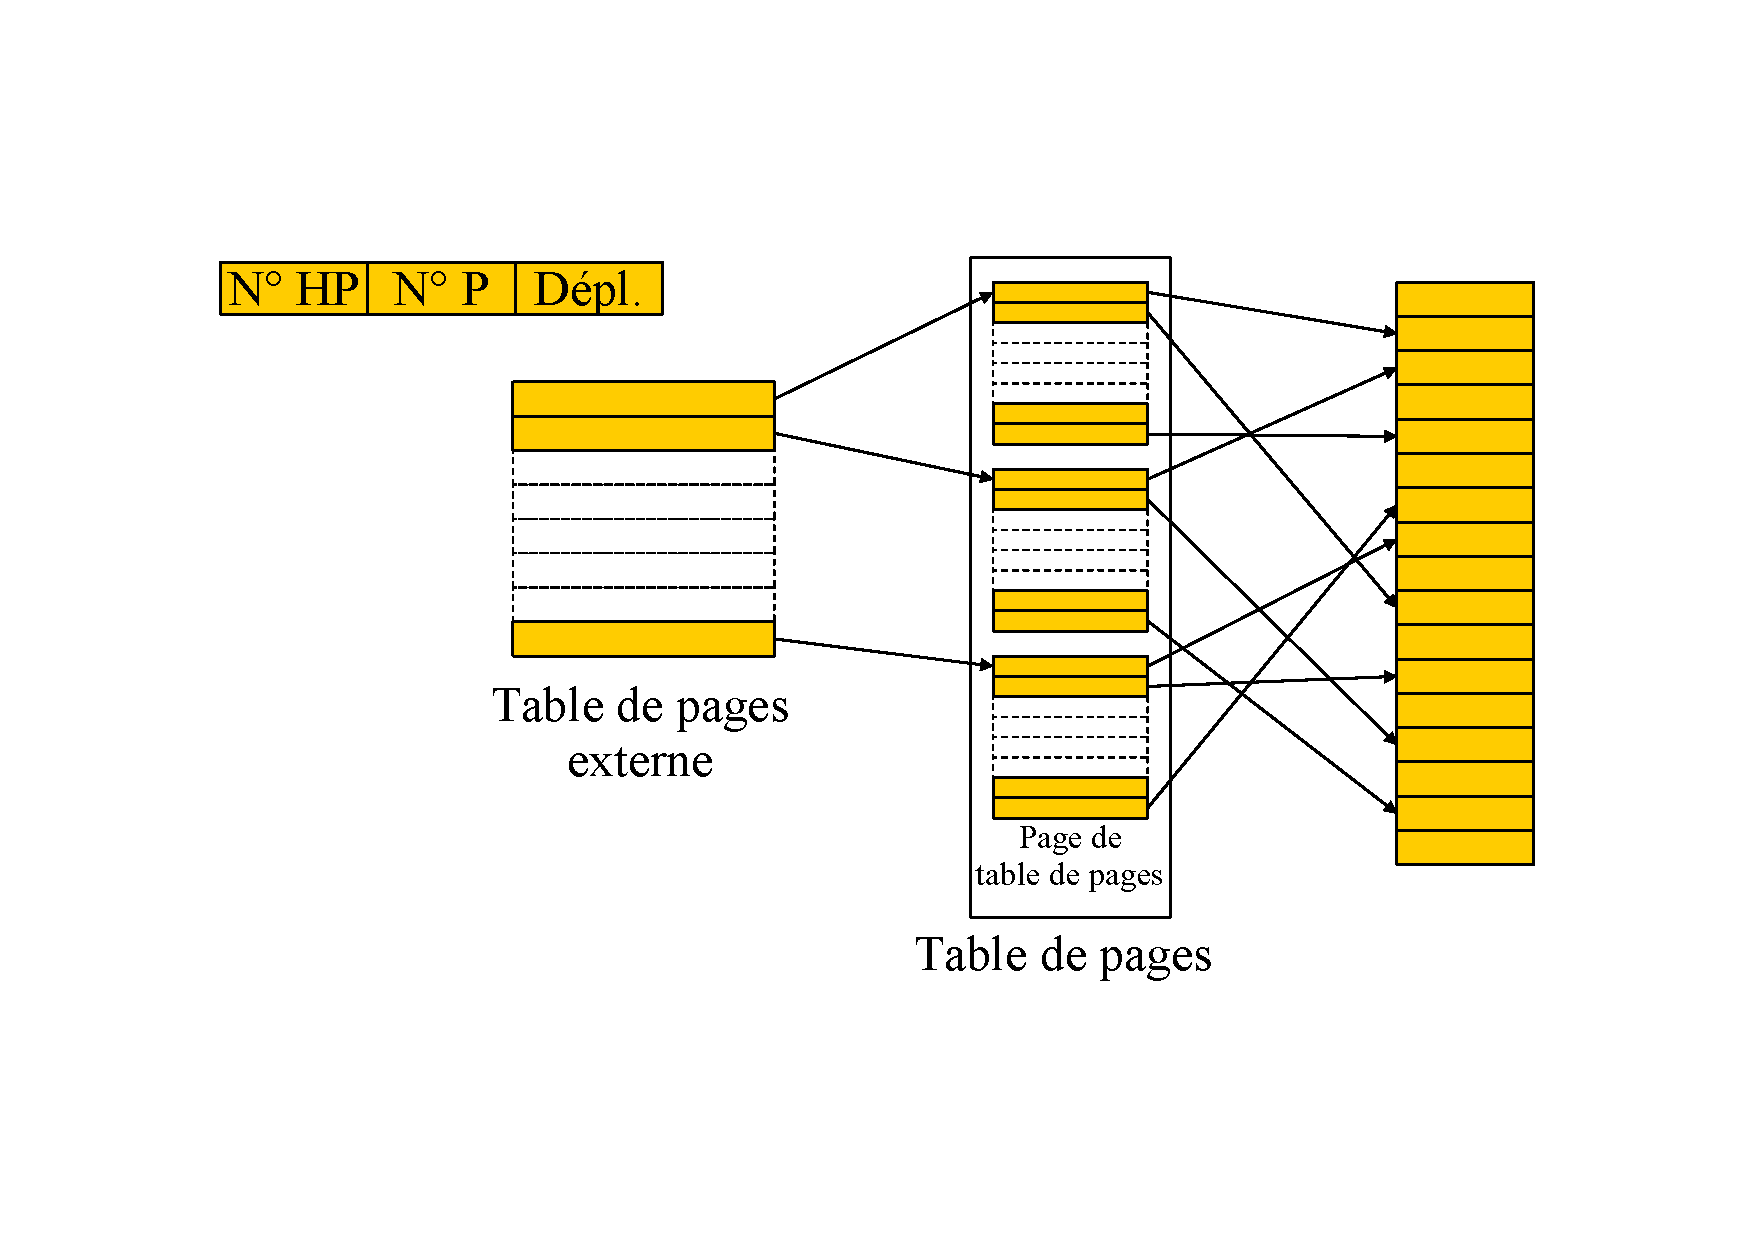
\includegraphics[width=\textwidth]{../illustration/pagination_2_niveaux.pdf}
\end{frame}


\begin{frame}
\frametitle{Pagination à deux niveaux}
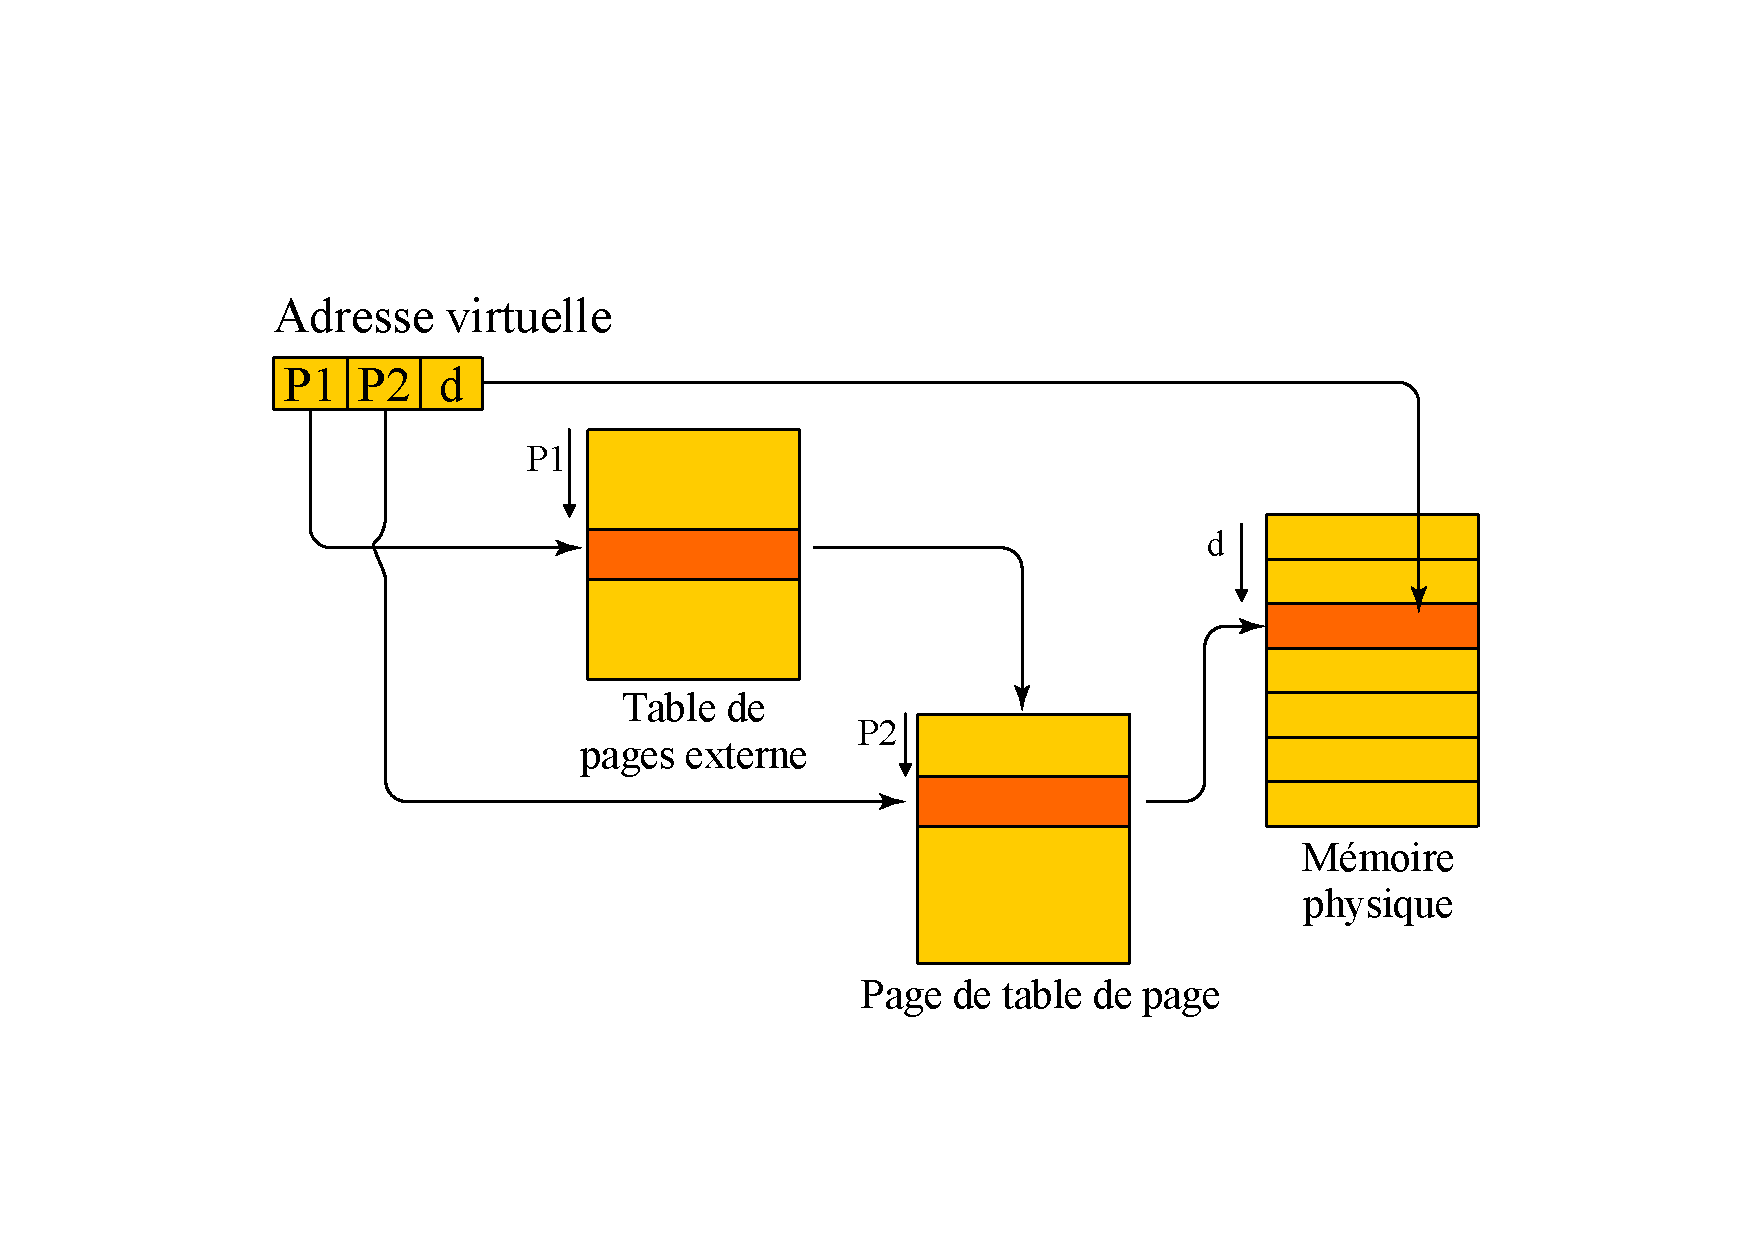
\includegraphics[width=\textwidth]{../illustration/memoire_paginee_deux_niveaux_calcul.pdf}
\end{frame}


\begin{frame}
\frametitle{Pagination à deux niveaux}
\begin{itemize}
\item La table des pages externes réside \textbf{toujours en mémoire principale}
\item Les tables de pages secondaires stockées dans des pages pouvant être \textbf{déplacées en mémoire secondaire}
\end{itemize}
\end{frame}


\begin{frame}
\frametitle{Optimisations liées à la pagination}
\begin{itemize}
\item Partage de données entre deux processus
\begin{itemize}
\item Utilisation de pages pointant vers la même case mémoire
\end{itemize}
\item Duplication de données entre deux processus
\begin{itemize}
\item Même mécanisme
\item Duplication des cases au plus tard :
\begin{itemize}
\item En cas de modification des données par un des deux processus (copy on write)
\end{itemize}
\end{itemize}
\end{itemize}
\end{frame}

\begin{frame}
\frametitle{Exemple : « copy on write » sur fork()}
\begin{itemize}
\item Duplication du contexte du processus :
\begin{itemize}
\item Les tables des pages des processus pères et fils font référence aux mêmes cadres,
\item Le premier processus écrivant dans une page provoque la duplication du cadre.
\end{itemize}
\item Les numéros de pages sont toujours différents, mais ils peuvent faire référence au mêmes cadres.
\end{itemize}
\end{frame}

\begin{frame}
\frametitle{Adresse Virtuelle $\rightarrow$ Adresse Physique}
\begin{itemize}
\item Calcul adresse réelle depuis adresse virtuelle :
\begin{itemize}
\item Num. page virtuelle $\rightarrow$ entrée de la TPV $\rightarrow$ Num. case physique
\item Déplacement identique pour les cases physiques et les pages virtuelles (même taille)
\item Si une page virtuelle n'est pas en mémoire physique $\rightarrow$ \textbf{défaut de page} (interruption)
\end{itemize}
\end{itemize}
\end{frame}


\begin{frame}
\frametitle{Adresse Virtuelle $\rightarrow$ Adresse Physique}
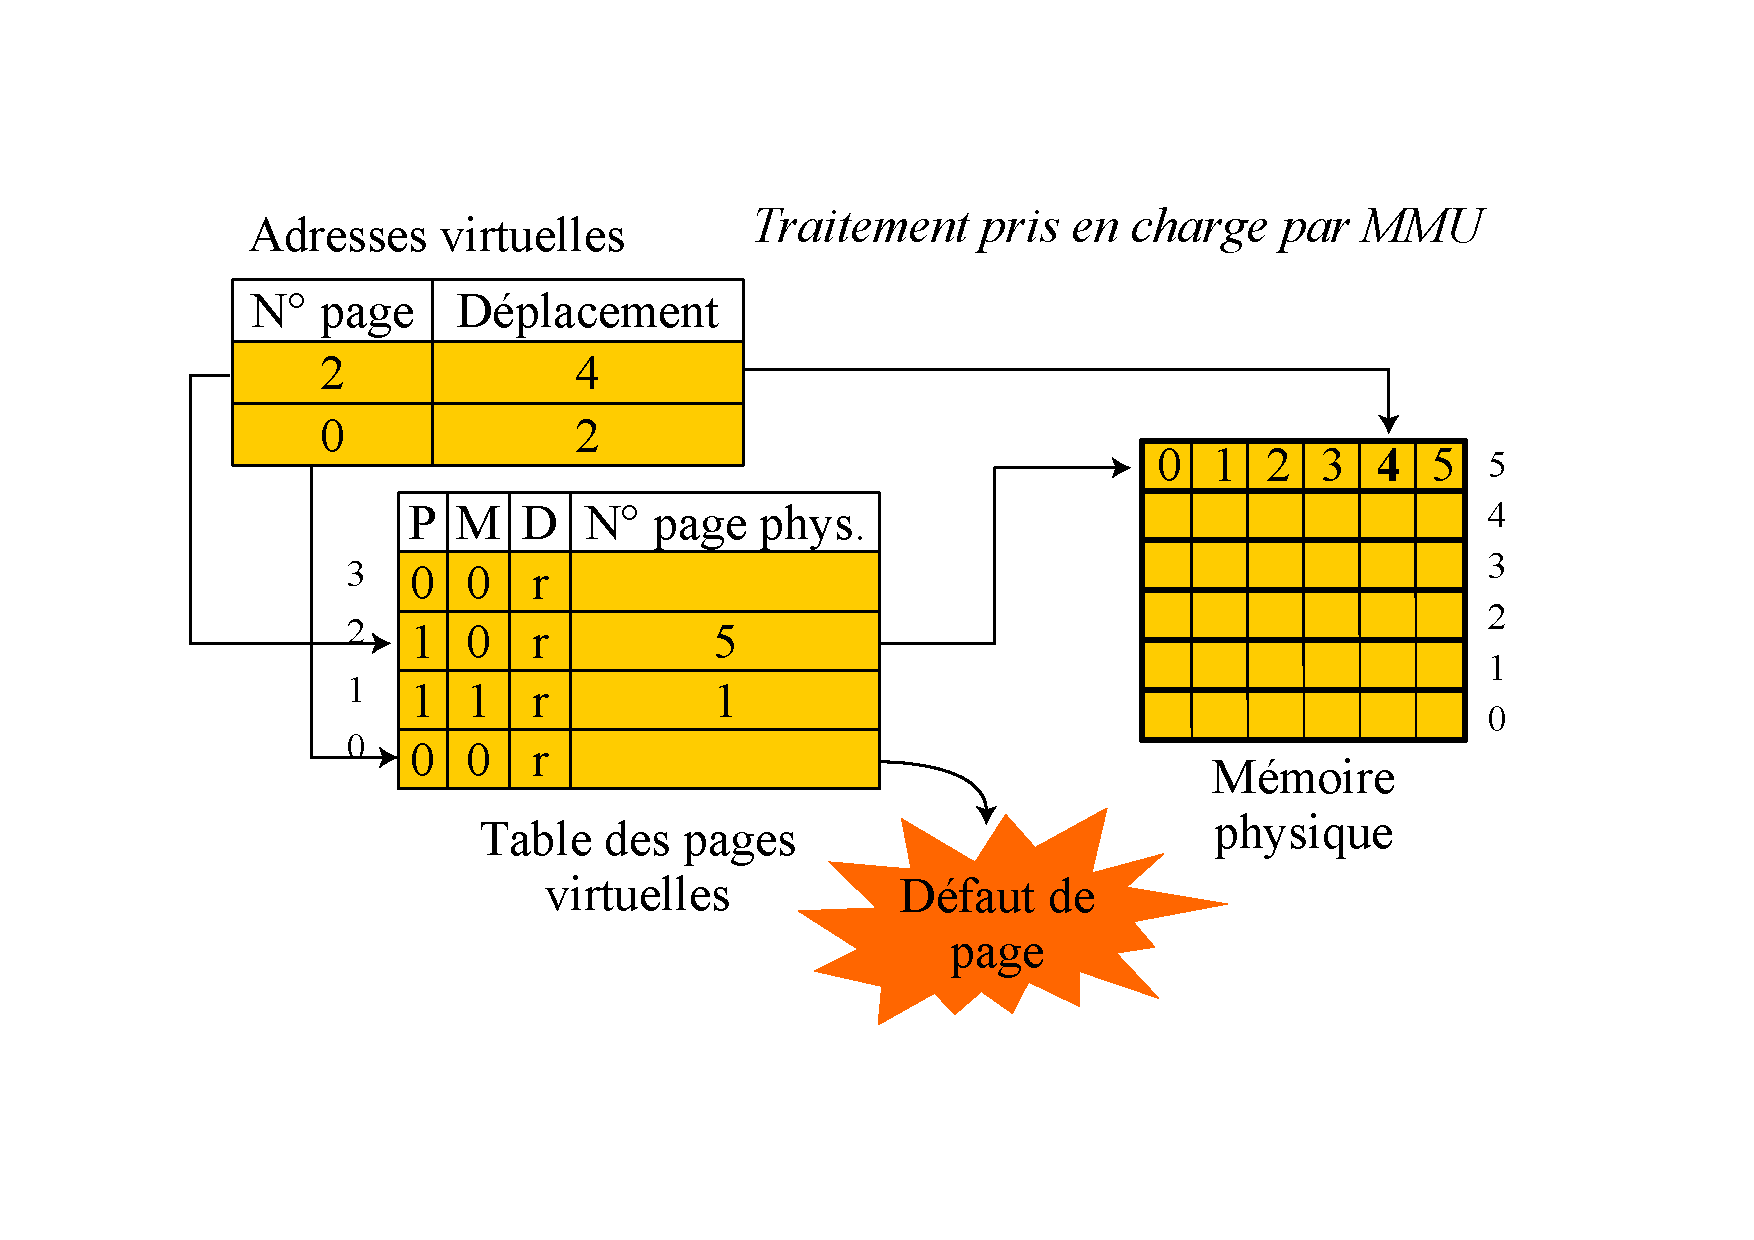
\includegraphics[width=\textwidth]{../illustration/table_pages_virtuelles_acces.pdf}
\end{frame}



\begin{frame}
\frametitle{Le défaut de page}
\begin{itemize}
\item Interruption levée lors de l'accès à une \textbf{page virtuelle non présente} en mémoire principale
\item Nécessite un traitement particulier
\begin{itemize}
\item Traitement du défaut de page
\item Consiste à charger en mémoire la page manquante
\begin{itemize}
\item E/S sur disque
\end{itemize}
\end{itemize}
\item Processus demandeur à l'état bloqué pendant le traitement du défaut de page

\end{itemize}
\end{frame}



\begin{frame}
\frametitle{Phases gestion défaut de page}
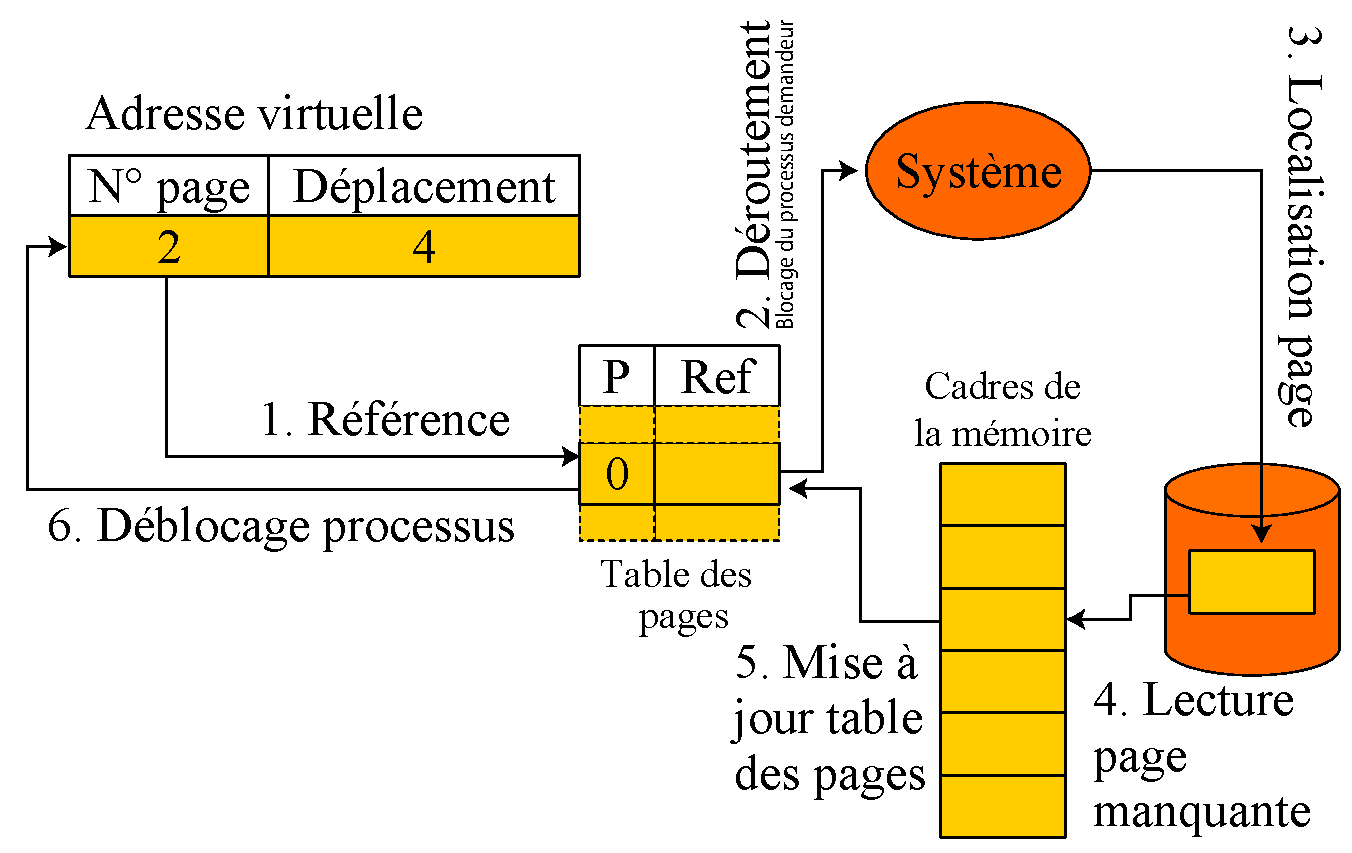
\includegraphics[width=\textwidth]{../illustration/traitement_defaut_page.pdf}
\end{frame}


\begin{frame}
\frametitle{Le défaut de page}
\begin{itemize}
\item Si au moins un cadre est libre en mémoire centrale
\begin{itemize}
\item Charger la page en défaut dans ce cadre
\end{itemize}
\item Sinon :
\begin{itemize}
\item Trouver un cadre non utilisé ou pouvant être considéré comme tel (victime)
\item Le libérer
\item Charger la page en défaut dans ce cadre
\end{itemize}
\end{itemize}

\end{frame}


\begin{frame}
\frametitle{Le défaut de page}
\begin{itemize}
\item Si la mémoire physique est pleine (\textbf{remplacement}) :
\begin{itemize}
\item Supprimer page m de la mémoire physique
\item Si la page m a été modifiée, la réécrire sur disque  
\item Modifier indicateur de présence en TPV de m
\end{itemize}
\item Puis, dans tous les cas :
\begin{itemize}
\item Charger la page référencée dans une case libre de la mémoire physique (\textbf{placement})
\item Modifier les indicateurs de présence en TPV
\end{itemize}
\end{itemize}
\end{frame}


\begin{frame}
\frametitle{Traitement d'un défaut de page}
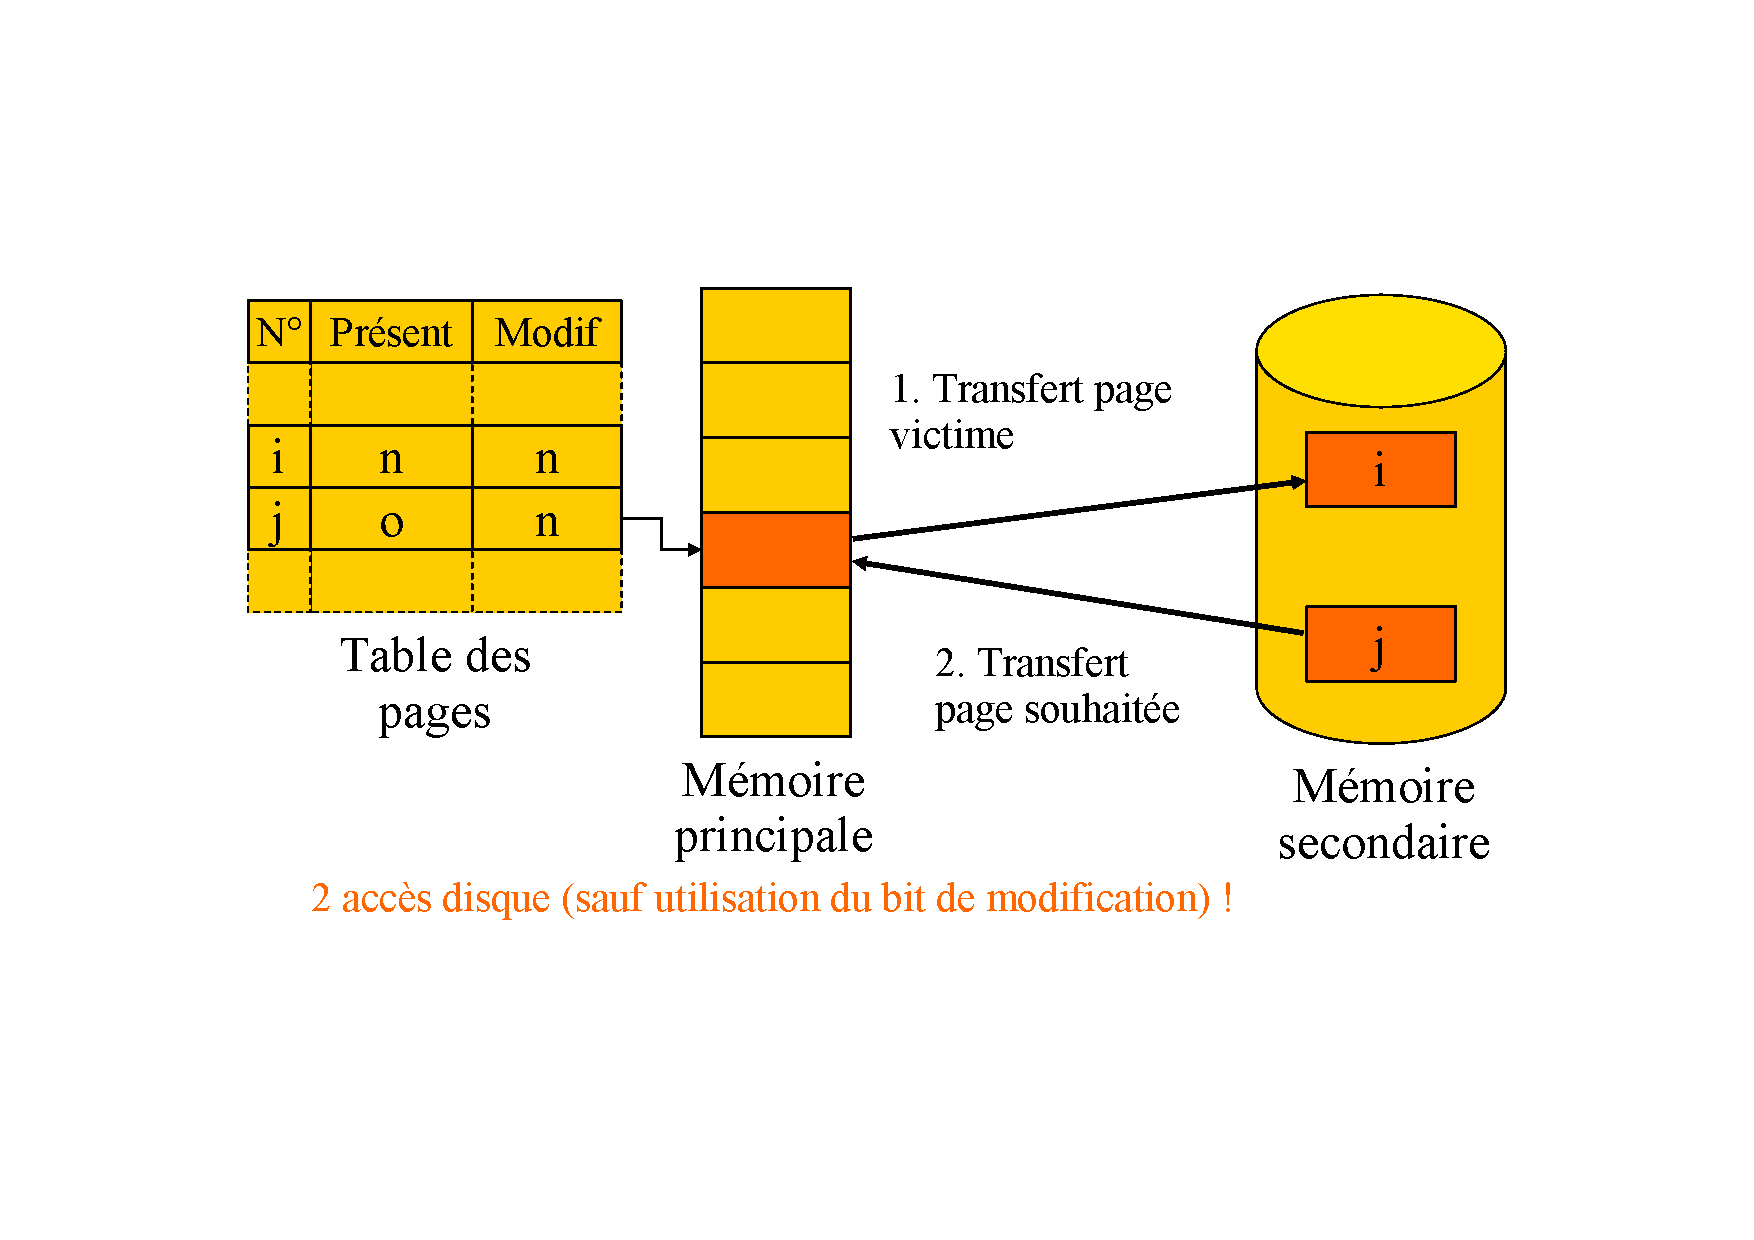
\includegraphics[width=\textwidth]{../illustration/traitement_defaut_page_remplacement.pdf}
\end{frame}


\begin{frame}
\frametitle{Pagination à la demande pure}
\begin{itemize}
\item Pagination à l'extrême :
\begin{itemize}
\item Possibilité de lancer l'exécution d'un processus dont aucune page ne réside en mémoire principale
\item Chargement des pages par le système d'exploitation au cours de l'exécution
\end{itemize}
\item Performances :
\begin{itemize}
\item Acceptables si le programme possède un lieu de référence
\end{itemize}
\end{itemize}
\end{frame}


\begin{frame}
\frametitle{Performances de la pagination à la demande}
\begin{itemize}
\item Temps d'accès :
\begin{itemize}
\item Accès direct :
\begin{itemize}
\item 100 nanosecondes
\end{itemize}
\item Traitement d'un défaut de page : 
\begin{itemize}
\item Qualification, changements contexte : $<$ 1 ms
\item 8 ms latence + 15 ms posit. + 1 ms transfert
\end{itemize}
\end{itemize}
\item Temps d'accès effectif :
\begin{itemize}
\item P : Probabilité d'un défaut de page
\item (1-P) x (accès mémoire) + P x (défaut page)
\end{itemize}
\end{itemize}
\end{frame}


\begin{frame}
\frametitle{Performances de la pagination à la demande}
\begin{itemize}
\item Temps d’accès effectif (page non modif.) :
\begin{itemize}
\item (1-P) x (accès mémoire) + P x (défaut page)
\item (1-P) x 100 + P x 25 000 000
\item 100 + 24 999 900 x P
\end{itemize}
\item Si $P = \frac{1}{1000}$
\begin{itemize}
\item Temps d'accès x 250
\end{itemize}
\item Pour variation $\le$ 10 \%
\begin{itemize}
\item $P \le \frac{1}{2500000}$
\end{itemize}
\end{itemize}
\end{frame}


\begin{frame}
\frametitle{Le pré-chargement : la localité}
\begin{itemize}
\item Optimisation du système :
\begin{itemize}
\item Tenir compte de la localité en pré-chargeant des pages avant d'en avoir besoin.
\end{itemize}
\item Localité :
\begin{itemize}
\item A un instant donné, les références observées dans un passé récent sont (en général) une bonne estimation des prochaines références
\item Non-uniformité :
\begin{itemize}
\item En moyenne, 75\% des références intéressent moins de 20\% des pages.
\end{itemize}
\end{itemize}
\end{itemize}
\end{frame}


\begin{frame}
\frametitle{Gestion de l'espace de permutation}
\begin{itemize}
\item E/S sur l'espace de permutation plus rapide que sur le reste du disque
\begin{itemize}
\item Manipulation de blocs :
\begin{itemize}
\item Entités de taille fixe
\item Entités de taille relativement importante lues en continu
\end{itemize}
\item Espace adressable directement
\begin{itemize}
\item Ne nécessite pas d'adressage indirect
\item Pas de consultation des informations en cours de lecture
\end{itemize}
\end{itemize}
\end{itemize}
\end{frame}



\begin{frame}
\frametitle{Choix victime - remplacement}
\begin{itemize}
\item Fondamental pour l'efficacité du système
\item Objectif du système :
\begin{itemize}
\item Minimiser les défauts de pages
\end{itemize}
\item Plusieurs stratégies sont possibles :
\begin{itemize}
\item Évincer la page la plus ancienne en mémoire
\begin{itemize}
\item Nécessite de connaître l'âge de chaque page
\end{itemize}
\item Évincer la page qui sera accédée le plus tard
\begin{itemize}
\item Nécessite une connaissance de ce qui va se passer
\end{itemize}
\end{itemize}
\end{itemize}
\end{frame}


\begin{frame}
\frametitle{Choix victime - remplacement}
\begin{itemize}
\item Idée :
\begin{itemize}
\item Remplacer la \textbf{page} qui sera \textbf{accédée le plus tard} (ou plus jamais, à l'extrême)
\end{itemize}
\item S'appuie sur un \textbf{support matériel} :
\begin{itemize}
\item Indispensable pour optimiser les algorithmes de remplacement
\item Ne doit pas pénaliser des performances
\item Renseignement sur les accès mémoire passés
\item Limitation aux seules fonctions disponibles
\end{itemize}
\end{itemize}
\end{frame}


\begin{frame}
\frametitle{Évaluation des algorithmes de remplacement}
\begin{itemize}
\item \textbf{Observation} du fonctionnement système
\item Comparaison avec algorithme optimal
\begin{itemize}
\item Théorique (nécessite de connaître le futur)
\item Basée sur une simulation
\end{itemize}
\item Critère de jugement des algorithmes :
\begin{itemize}
\item Nombre de défaut de pages générés
\item Le plus proche possible de l'algorithme optimal
\end{itemize}
\end{itemize}
\end{frame}


\begin{frame}
\frametitle{Évaluation des algorithmes de remplacement}
\begin{itemize}
\item Extraction de la liste les appels mémoire :
\begin{itemize}
\item Grande quantité d'informations
\begin{itemize}
\item de l'ordre de 1 000 000 références par seconde
\end{itemize}
\item Stockage des seuls numéros de page
\item Stockage des premières références
\end{itemize}
\item Chaîne de référence :
\begin{itemize}
\item Générée aléatoirement 
\item Observation système
\end{itemize}
\end{itemize}
\end{frame}


\begin{frame}
\frametitle{Évaluation des algorithmes de remplacement}
\begin{exampleblock}{Chaîne de référence}
\begin{itemize}
\item Num. page sur 2, déplacement sur 2
\item \texttt{0710, 0711, 0756... 0045, 0046, 0047... 0126... 0201, 0202, 0203... 0025, 0314, 0015, 0422, 0218, 0365, 0070, 0312, 0206, 0168, 0269, 0010, 0102, 0700, 0085, 0112}
\end{itemize}
\end{exampleblock}
\begin{itemize}
\item Après simplification :
\begin{itemize}
\item \texttt{7, 0, 1, 2, 0, 3, 0, 4, 2, 3, 0, 3, 2, 1, 2, 0, 1, 7, 0, 1}
\end{itemize}
\item Doit connaître le nombre de cadres de page disponibles
\end{itemize}
\end{frame}


\begin{frame}
\frametitle{Évaluation des algorithmes de remplacement}
\begin{itemize}
\item Basé sur un Scénario
\item Utilisation de la chaîne de référence suivante :
\begin{itemize}
\item \texttt{7, 0, 1, 2, 0, 3, 0, 4, 2, 3, 0, 3, 2, 1, 2, 0, 1, 7, 0, 1}
\end{itemize}
\item Trois cadres de page\footnote{Cas d'école très éloigné de la réalité}
\end{itemize}
\end{frame}


\begin{frame}
\frametitle{Algorithmes de remplacement possibles}
\begin{block}{Algorithmes les plus courants}
\begin{tabular}{c|l}
\textbf{MIN} & Algorithme optimal \\
\textbf{FIFO} \begin{tiny}(First In First Out)\end{tiny}& Ordre chronologique de chargement \\
\textbf{LRU} \begin{tiny}(Least Recently Used)\end{tiny} & Ordre chronologique d'utilisation \\
\textbf{FINUFO} \begin{tiny}(First In Not Used, First Out)\end{tiny} & Approximation du LRU \\
\textbf{LFU} \begin{tiny}(Least Frequently Used)\end{tiny} & La moins utilisée \\
\textbf{Random} & Au hasard \\
\end{tabular}
\end{block}
\end{frame}


\begin{frame}
\frametitle{Algorithme optimal}
\begin{itemize}
\item Algorithme \textbf{OPT} ou \textbf{MIN} :
\begin{itemize}
\item Remplacer la page qui sera utilisée le plus tard possible (ou jamais)
\end{itemize}
\item Garantit le plus faible taux de défaut de page
\item Difficile à mettre en œuvre :
\begin{itemize}
\item Nécessite de connaître le comportement futur des processus
\item Référence pour évaluation des algorithmes
\end{itemize}
\end{itemize}
\end{frame}



\begin{frame}
\frametitle{Algorithme de remplacement optimal}
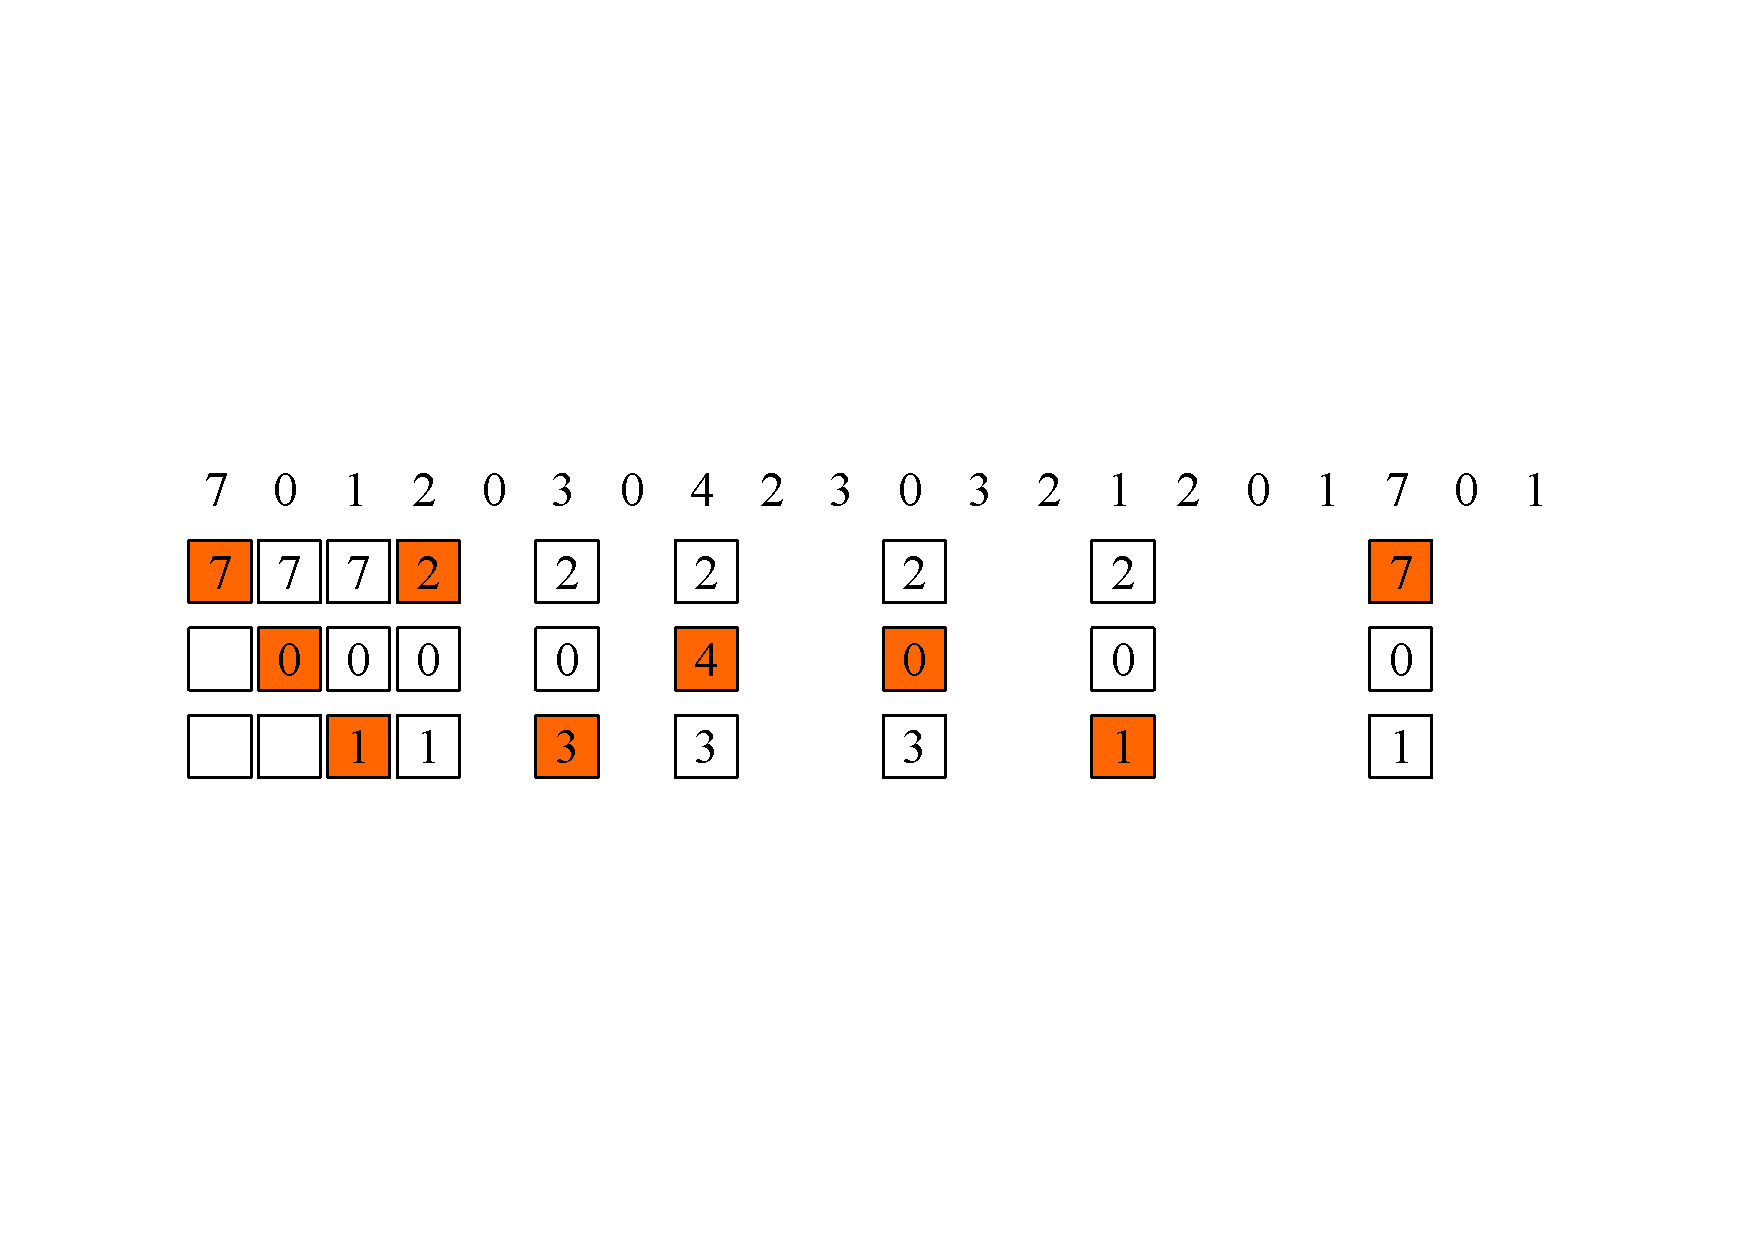
\includegraphics[width=\textwidth]{../illustration/remplacement_opt.pdf}
\center{9 défauts de page}
\end{frame}


\begin{frame}
\frametitle{Algorithme FIFO}
\begin{itemize}
\item Association, pour chaque page :
\begin{itemize}
\item Date de chargement en mémoire principale
\end{itemize}
\item Choix d'une victime :
\begin{itemize}
\item Choix de la page la plus ancienne
\end{itemize}
\item Implémentations possibles :
\begin{itemize}
\item Date sur chaque chargement de cadre
\item Liste FIFO des pages chargées en mémoire
\end{itemize}
\end{itemize}
\end{frame}


\begin{frame}
\frametitle{Algorithme FIFO}
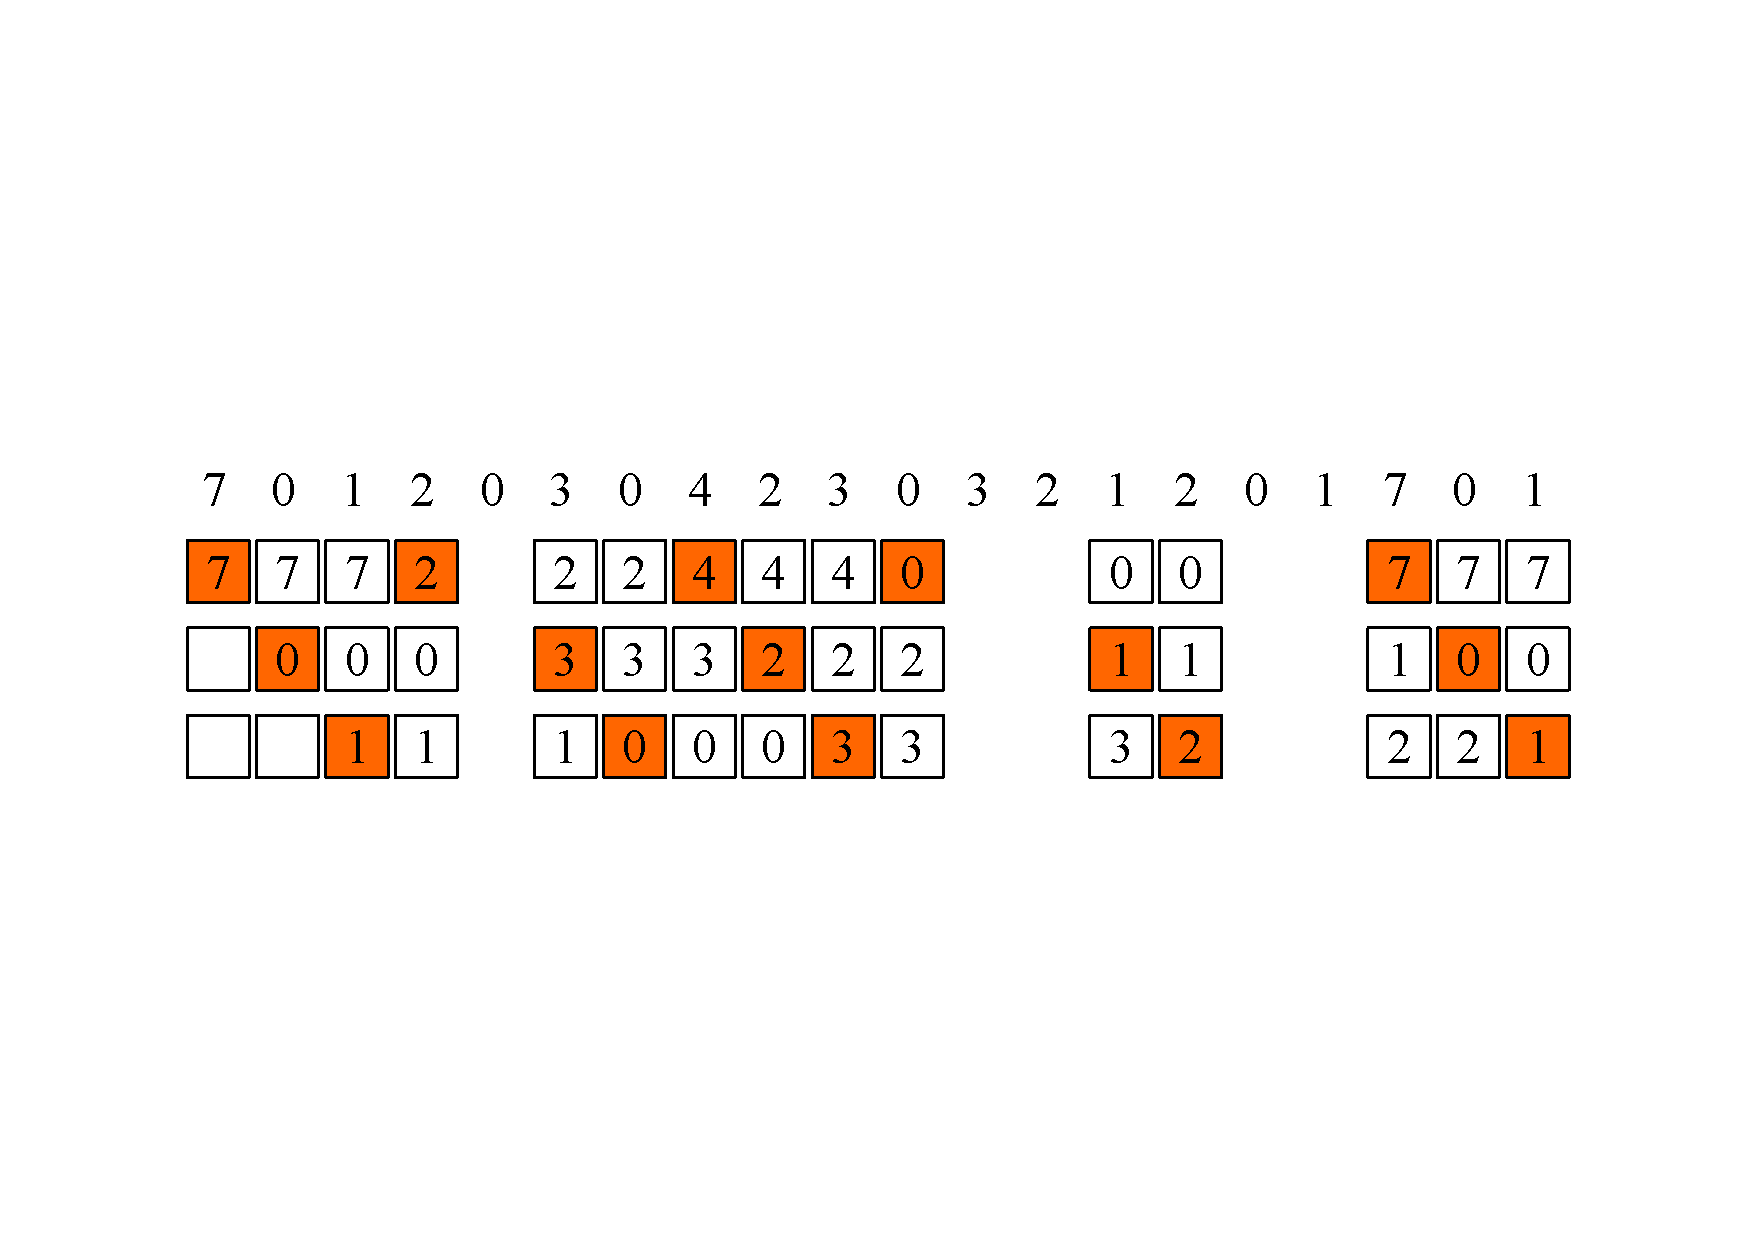
\includegraphics[width=\textwidth]{../illustration/remplacement_fifo.pdf}
\center{15 défauts de page}
\end{frame}


\begin{frame}
\frametitle{Algorithme FIFO}
\begin{itemize}
\item Résultats mauvais dans le cas d'une page chargée tôt et accédée souvent
\begin{itemize}
\item Exemple : Variables souvent utilisées
\item Augmente le nombre de défaut de page
\end{itemize}
\item Anomalie de Belady
\begin{itemize}
\item Le nombre de défaut de page peut croître en même temps que le nombre de cadres allouées
\end{itemize}
\end{itemize}
\end{frame}

\begin{frame}
\frametitle{Anomalie de Belady}
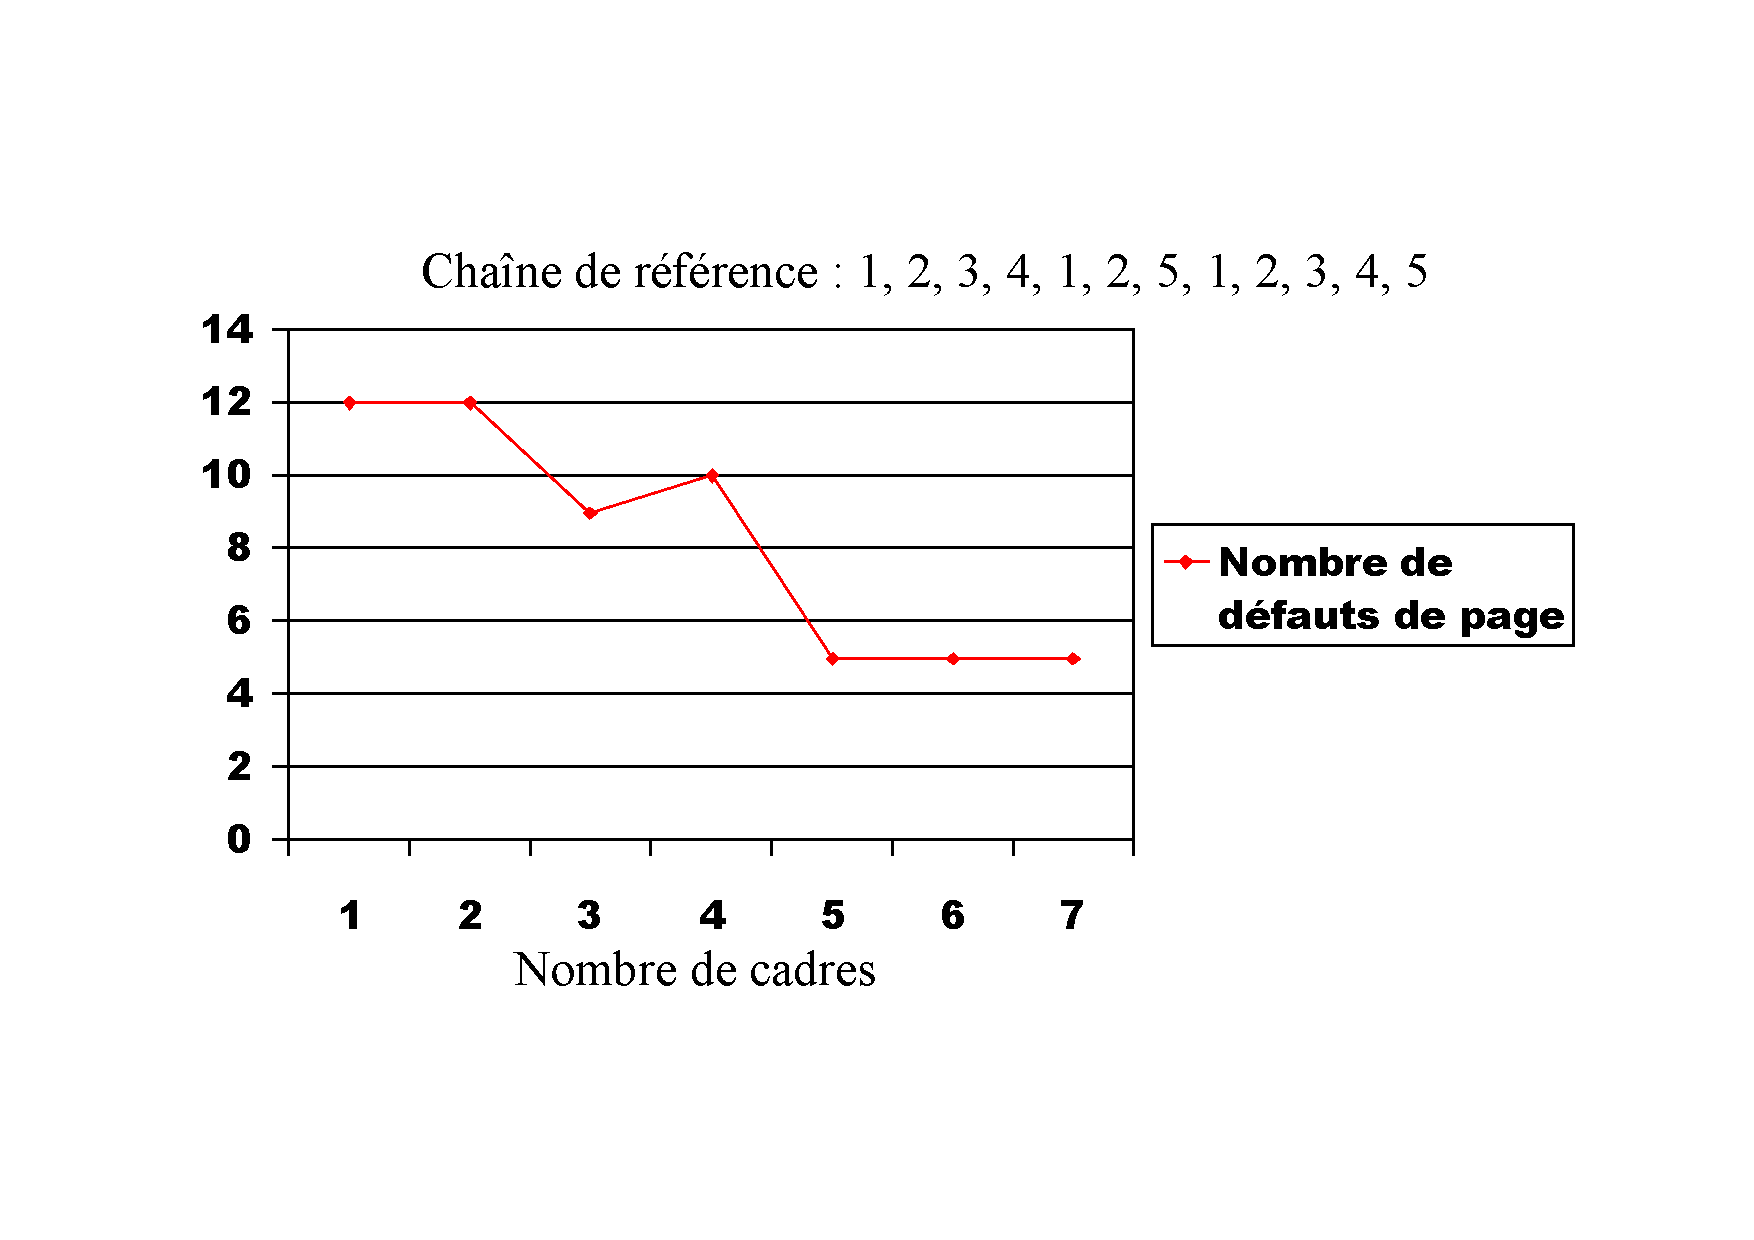
\includegraphics[width=\textwidth]{../illustration/remplacement_fifo_belady.pdf}
\end{frame}


\begin{frame}
\frametitle{Algorithme LRU}
\begin{itemize}
\item Victime : Page moins récemment utilisée
\item Approximation de MIN - OPT
\item Se base sur l'hypothèse de localité :
\begin{itemize}
\item A un instant donné, les références observées dans un passé récent sont (en général) une bonne estimation des prochaines références
\end{itemize}
\item Une page accédée récemment à de fortes chances d'être utilisée dans un avenir proche
\end{itemize}
\end{frame}


\begin{frame}
\frametitle{Algorithme LRU}
\begin{itemize}
\item Association à chaque page de la date de dernière utilisation
\begin{itemize}
\item Compteur - horloge
\item Pile (déplacement des pages utilisées au sommet)
\end{itemize}
\item Victime :
\begin{itemize}
\item Page moins récemment utilisée
\end{itemize}
\item Algorithme performant en pratique
\begin{itemize}
\item Bien meilleur que FIFO
\end{itemize}
\end{itemize}
\end{frame}


\begin{frame}
\frametitle{Algorithme LRU}
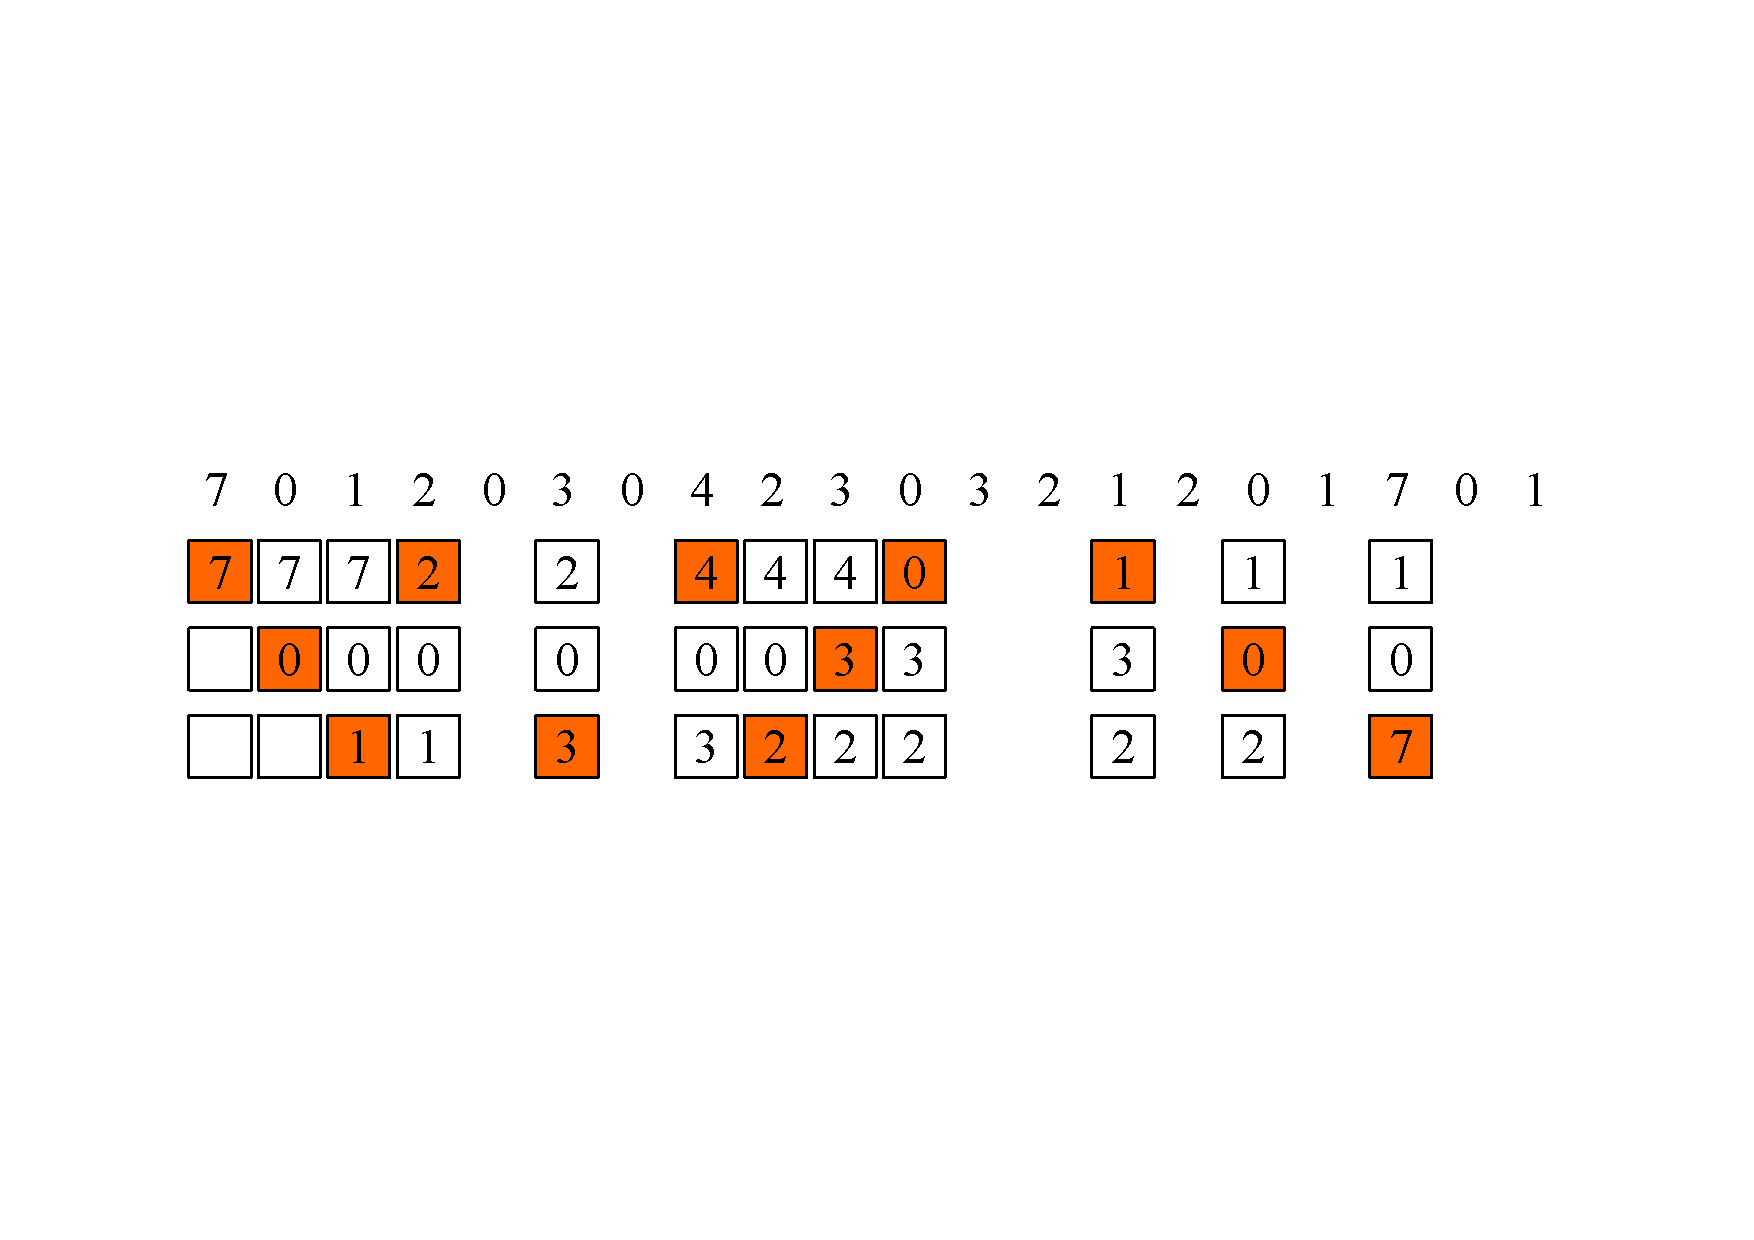
\includegraphics[width=\textwidth]{../illustration/remplacement_lru.pdf}
\center{12 défauts de page}
\end{frame}


\begin{frame}
\frametitle{Implémentation de l'algorithme LRU}
\begin{itemize}
\item Assistance matérielle conséquente :
\begin{itemize}
\item Compteur :
\begin{itemize}
\item Date associée à chaque entrée de la TPV
\item Horloge incrémentée à chaque référence mémoire
\item Remplacement page dont le compteur est le plus faible 
\end{itemize}
\item Pile :
\begin{itemize}
\item Pile des numéros de page
\item Déplacement d'une page au sommet à chaque référence
\item Base de la pile : LRU
\end{itemize}
\end{itemize}
\end{itemize}
\end{frame}


\begin{frame}
\frametitle{LRU : Implémentation du compteur}
\begin{itemize}
\item Nécessite la consultation de toute la table des pages pour trouver la LRU
\item Écriture dans la table des pages à chaque accès mémoire
\item Entretient du compteur d'horloge
\end{itemize}
\end{frame}


\begin{frame}
\frametitle{LRU : Implémentation de la pile}
\begin{itemize}
\item Déplacement de pages depuis le milieu de la pile vers le sommet
\item Liste double chaînée
\begin{itemize}
\item Pointeur vers la tête de la liste
\item Pointeur vers la queue de la liste
\end{itemize}
\item Mise à jour contraignante
\item Recherche LRU directe
\end{itemize}
\end{frame}


\begin{frame}
\frametitle{LRU : Implémentation de la pile}
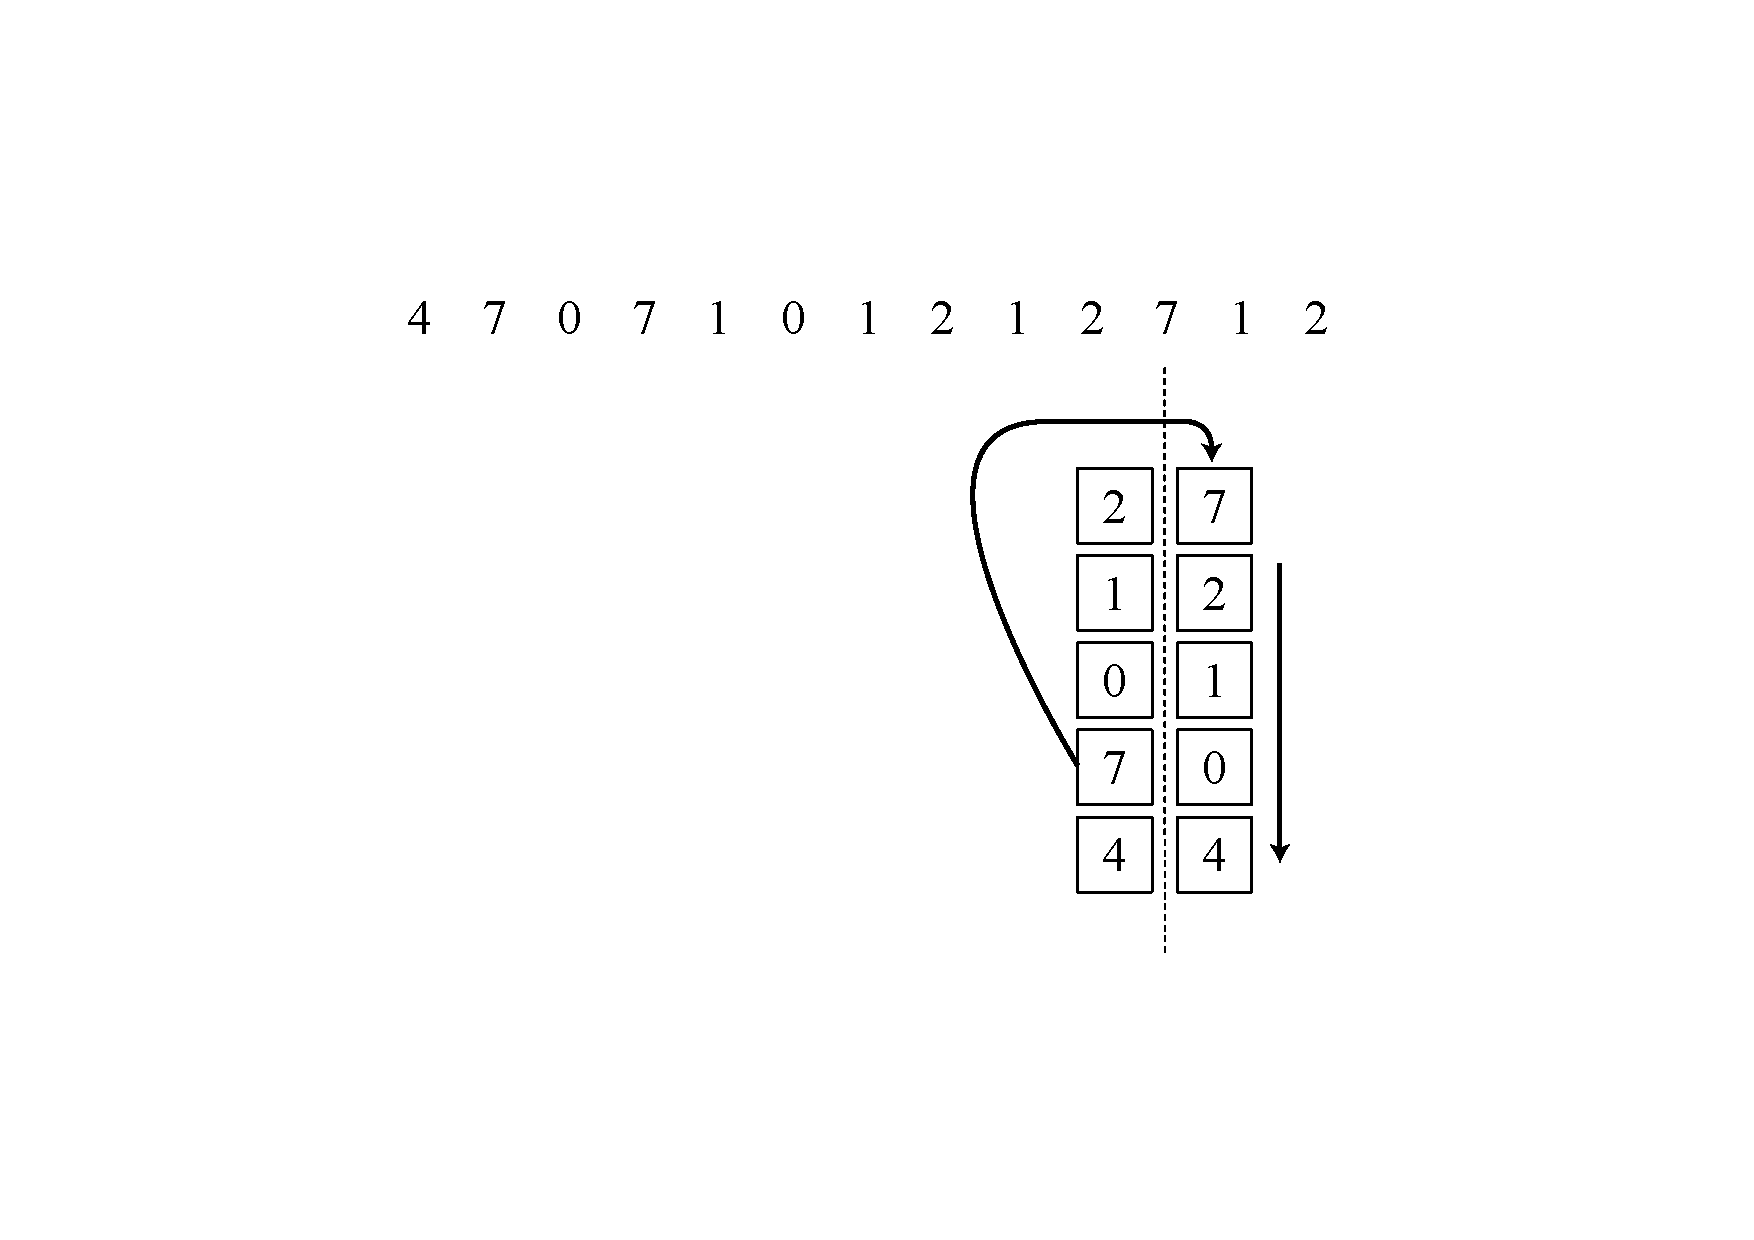
\includegraphics[width=.8\textwidth]{../illustration/remplacement_lru_pile.pdf}
\end{frame}


\begin{frame}
\frametitle{LRU : Implémentation de la pile}
\begin{itemize}
\item Ne peut jamais présenter l'anomalie de Belady
\item Car on a toujours :
\begin{itemize}
\item L'ensemble des pages en mémoire de n cadres est toujours un sous-ensemble des pages qui se trouveraient en mémoire avec n+1 cadres de page.
\end{itemize}
\end{itemize}
\end{frame}


\begin{frame}
\frametitle{Algorithme LRU}
\begin{itemize}
\item Pas réalisable sans assistance matérielle avancée
\begin{itemize}
\item Traitement par interruptions système possible avec fortes pertes (facteur 10 au minimum)
\end{itemize}
\item Pour le compteur :
\begin{itemize}
\item Mise à jour du compteur d'horloge
\item Parcours de la table des pages
\end{itemize}
\item Pour la pile :
\begin{itemize}
\item Mise à jour de la pile
\end{itemize}
\end{itemize}
\end{frame}


\begin{frame}
\frametitle{Algorithmes d'approximation LRU}
\begin{itemize}
\item LRU coûteux
\begin{itemize}
\item Nécessite support matériel spécifique et complexe
\end{itemize}
\item Utilisation bit de référence de la table des pages
\begin{itemize}
\item Initialisés à 0
\item Positionné à 1 à chaque référence au cadre
\begin{itemize}
\item par le matériel (MMU)
\end{itemize}
\item Permet de distinguer les pages non utilisées 
\end{itemize}
\end{itemize}
\end{frame}


\begin{frame}
\frametitle{LRU + bits de référence supplémentaire}
\begin{itemize}
\item Utilisation d'un ensemble de bits de référence (un octet, par exemple)
\begin{itemize}
\item Initialisé à \texttt{00000000}
\item Mise à 1 du bit de référence lors de l'accès à la page
\begin{itemize}
\item \texttt{00000000} $\rightarrow$ \texttt{10000000}
\end{itemize}
\item Décalage régulier du bit de référence vers la droite (arbitrairement)
\begin{itemize}
\item \texttt{10000000} $\rightarrow$ \texttt{01000000}
\end{itemize}
\end{itemize}
\end{itemize}

\end{frame}


\begin{frame}
\frametitle{LRU + bits de référence supplémentaire}
\begin{itemize}
\item Page jamais utilisée depuis 8 périodes :
\begin{itemize}
\item \texttt{00000000}
\end{itemize}
\item Page utilisée au moins une fois dans chacune des 8 dernières périodes
\begin{itemize}
\item \texttt{11111111}
\end{itemize}
\item Comparaison de pages :
\begin{itemize}
\item \texttt{11000100} plus récemment utilisée que \texttt{01110111}
\end{itemize}
\end{itemize}
\end{frame}


\begin{frame}
\frametitle{Algorithme de la seconde chance}
\begin{itemize}
\item Utilisation d'un algorithme FIFO
\item Prise en compte du bit de référence
\item Choix de la victime :
\begin{itemize}
\item Utilisation FIFO
\item Si bit de référence = 1
\begin{itemize}
\item Bit = 0, date d'arrivée = date courante
\item Choix de la page suivante
\end{itemize}
\item Si bit de référence = 0
\begin{itemize}
\item Remplacement de la page
\end{itemize}
\end{itemize}
\end{itemize}
\end{frame}


\begin{frame}
\frametitle{Seconde chance - liste circulaire}
\begin{itemize}
\item Liste circulaire
\item Bit de référence
\item Choix d'une victime :
\begin{itemize}
\item Parcours de la liste jusqu'à une page pour laquelle le bit de référence = 0
\item Effacement du bit de référence lors du parcours
\end{itemize}
\end{itemize}
\end{frame}


\begin{frame}
\frametitle{Seconde chance - liste circulaire}
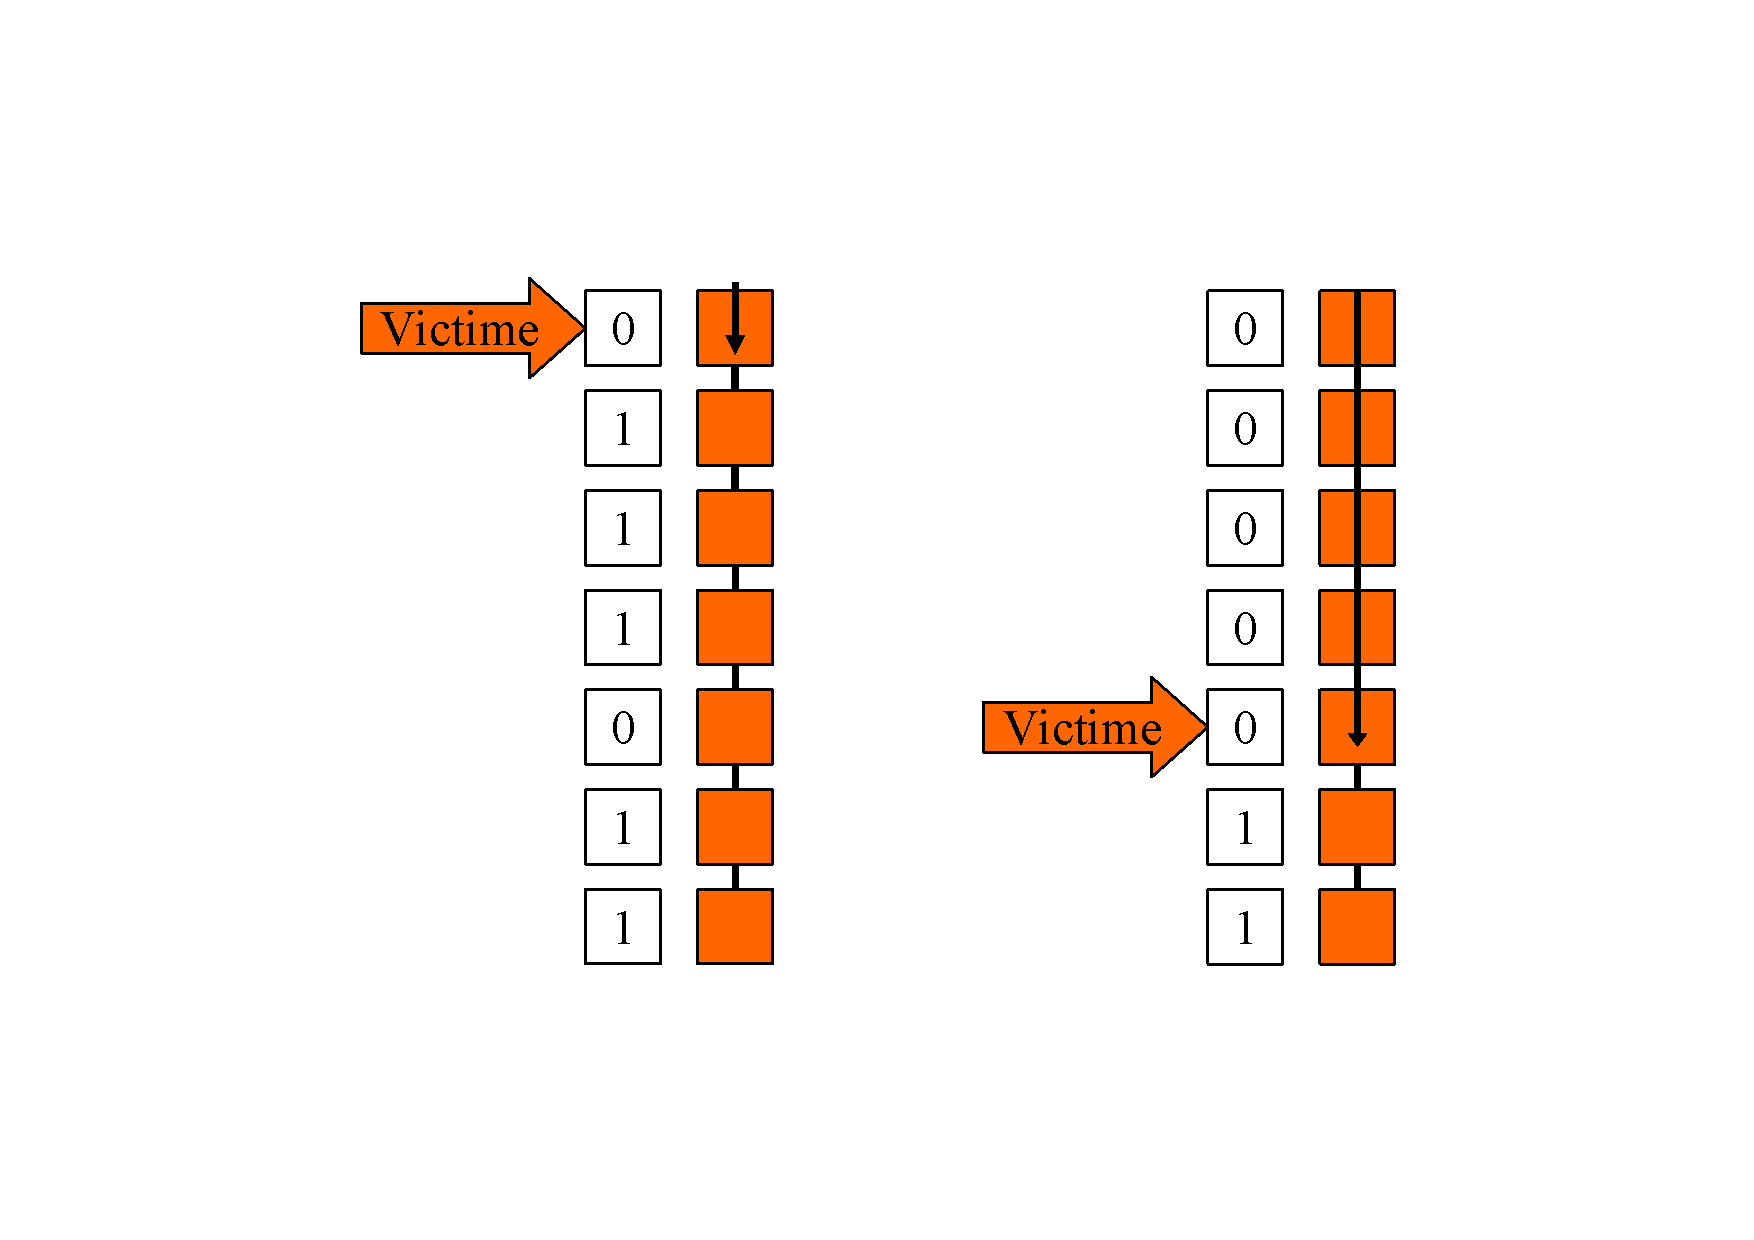
\includegraphics[width=.8\textwidth]{../illustration/remplacement_seconde_chance_liste.pdf}
\end{frame}

\begin{frame}
\frametitle{Algorithme de la seconde chance amélioré}
\begin{itemize}
\item Prise en compte du bit de modification
\begin{itemize}
\item \texttt{(0, 0)} : Ni récemment utilisée, ni modifiée
\begin{itemize}
\item Meilleure page à remplacer
\end{itemize}
\item \texttt{(0, 1)} : Pas récemment utilisée, mais modifiée
\begin{itemize}
\item Coûteuse à remplacer (doit écrire la page)
\end{itemize}
\item \texttt{(1, 0)} : Récemment utilisée, non modifiée
\begin{itemize}
\item Sera certainement utilisée prochainement
\end{itemize}
\item \texttt{(1, 1)} : Récemment utilisée, modifiée
\begin{itemize}
\item Sera certainement utilisée prochainement
\end{itemize}
\end{itemize}
\end{itemize}
\end{frame}


\begin{frame}
\frametitle{Algorithme de la seconde chance amélioré}
\begin{itemize}
\item Permet de réduire les accès disque en privilégiant les pages ne nécessitant pas de mise à jour en mémoire secondaire
\item Utilisé par le système de gestion de la mémoire virtuelle du Macintosh
\begin{itemize}
\item $\rightarrow$ MacOs 9
\end{itemize}
\end{itemize}
\end{frame}


\begin{frame}
\frametitle{Algorithmes à base de comptage}
\begin{itemize}
\item Compteur mis à jour à chaque accès
\item \textbf{LFU} : Page la moins fréquemment utilisée
\begin{itemize}
\item Choix page ayant le plus faible compteur
\item Décalage régulier compteur : dégradation exponentielle
\end{itemize}
\item \textbf{MFU} : Page la plus fréquemment utilisée
\begin{itemize}
\item Choix page dont le compteur est le plus élevé
\item Compteur faible : Chargement mémoire récent $\rightarrow$ probabilité accès futur
\end{itemize}
\end{itemize}
\end{frame}


\begin{frame}
\frametitle{Algorithmes à base de comptage}
\begin{itemize}
\item Implémentation exigeante
\begin{itemize}
\item Mise à jour de la TPV à chaque accès
\item Parcours de l'ensemble de la TPV pour recherche de la victime
\item Fonction de comparaison complexe
\end{itemize}
\item Peu efficace :
\begin{itemize}
\item Se rapproche rarement de l’algorithme optimal
\end{itemize}
\item Rarement utilisé
\end{itemize}
\end{frame}


\begin{frame}
\frametitle{Algorithme mise en tampon de pages}
\begin{itemize}
\item Utilisé \textbf{en complément} d'un autre algorithme
\item \textbf{Réserve} de cadres de pages libres
\item Lecture des cadres disque vers cadre de la réserve avant recopie de la victime sur disque
\begin{itemize}
\item Permet de redonner plus vite la main au processus (sans attendre la fin de l'écriture)
\end{itemize}
\end{itemize}
\end{frame}


\begin{frame}
\frametitle{Algorithme mise en tampon de pages}
\begin{itemize}
\item Lorsque la victime est enregistrée sur disque, son cadre est attribué à la réserve
\item Possibilité de mémoriser le numéro de page contenu dans les cadres de la réserve (réutilisation possible sans E/S)
\item Extension possible :
\begin{itemize}
\item Entretient de la liste des pages modifiées
\item Dès que le systèmes est inactif, recopie des pages modifiées sur disque
\end{itemize}
\end{itemize}
\end{frame}


\begin{frame}
\frametitle{Algorithme mise en tampon de pages}
\begin{itemize}
\item Utilisé dans le système VAX/VMS avec un algorithme de remplacement FIFO
\item Possibilité de réutiliser des pages malencontreusement effacées
\item Algorithme simple et efficace
\begin{itemize}
\item Peut s'exécuter sans support matériel sophistiqué
\item Pas de bit de référence dans les premiers VAX
\end{itemize}
\end{itemize}
\end{frame}

\begin{frame}
\frametitle{Choix victime : Conclusion}
\begin{itemize}
\item Remarques :
\begin{itemize}
\item OPT non réalisable en pratique
\item FIFO : Mauvais résultats 
\begin{itemize}
\item page chargée tôt et accédée souvent
\item variables globales
\end{itemize}

\item Bon résultats en se basant sur la date de dernier accès, et/ou la fréquence d'accès :
\begin{itemize}
\item LRU, LFU
\end{itemize}
\end{itemize}
\item Nécessite comptabilité des accès
\begin{itemize}
\item Extrêmement coûteux
\item Utilisation d'approximations
\end{itemize}
\end{itemize}
\end{frame}


\begin{frame}
\frametitle{Problème de la répartition des cadres de page}
Système mono-utilisateur :
\begin{itemize}
\item Utilisation de tous les cadres de pages disponibles pour répondre au besoins de l'utilisateur
\item Un processus reçoit n'importe quel cadre de page libre
\begin{itemize}
\item Utilisation de toute la mémoire nécessaire (dans la mesure des disponibilités)
\item Ne pénalise que les processus de l'utilisateur
\end{itemize}
\end{itemize}
\end{frame}


\begin{frame}
\frametitle{Problème de la répartition des cadres de page}
Système multi-programmé :
\begin{itemize}
\item Partage de la mémoire entre plusieurs programmes et utilisateurs
\item Risque :
\begin{itemize}
\item Monopolisation de la mémoire par un utilisateur
\end{itemize}
\item Contraintes :
\begin{itemize}
\item Nombre minimum de pages allouées à chaque processus
\item Compétition pour obtenir des cadres de pages
\item Partage équitable de la mémoire
\end{itemize}
\end{itemize}
\end{frame}


\begin{frame}
\frametitle{Algorithmes de remplacement}
\begin{itemize}
\item But :
\begin{itemize}
\item Permettre le choix d'une victime lors du traitement d'un défaut de page
\end{itemize}
\item Contraintes :
\begin{itemize}
\item Utilisation optimale de la mémoire disponible
\item Limiter les perturbations inter-processus (éviter au maximum qu'un processus soit perturbé par le déroulement d'un autre)
\end{itemize}
\end{itemize}
\end{frame}


\begin{frame}
\frametitle{Portée des algorithmes de remplacement}
\begin{itemize}
\item Remplacement local :
\begin{itemize}
\item Cloisonné pour chaque processus
\item Choix victime parmi les cadres du processus
\end{itemize}
\item Remplacement global :
\begin{itemize}
\item L'algorithme porte sur l'ensemble des pages du système
\item Choix victime parmi tous les cadres du système
\item Possibilité de pénaliser un autre processus
\end{itemize}
\end{itemize}
\end{frame}


\begin{frame}
\frametitle{Algorithme de remplacement global}
\begin{itemize}
\item Choix victime parmi tous les cadres mémoire
\item Variation du nombre de cadres de pages alloués à chaque processus
\item Permet d'ajuster l'espace mémoire des processus en fonction de leurs besoins
\end{itemize}
\end{frame}


\begin{frame}
\frametitle{Algorithme de remplacement global}
\begin{itemize}
\item Taux de défaut de page difficile à contrôler au niveau du processus :
\begin{itemize}
\item Fonction de l'allocation des autres processus
\item Variation importante des temps de réponse pour des raisons extérieures au processus
\end{itemize}
\item Utilisation efficace de la mémoire 
\item Adapté aux processus ayant des besoins mémoire pouvant varier dans le temps
\end{itemize}
\end{frame}


\begin{frame}
\frametitle{Algorithme de remplacement local}
\begin{itemize}
\item Chaque processus ne peut sélectionner une victime que parmi ses propres cadres
\item Nombre de cadres de pages alloués constant pour chaque processus
\item Permet de contrôler le taux de défaut de page au niveau de chaque processus
\begin{itemize}
\item Un processus gourmand en mémoire ne peut pas faire augmenter le taux de défaut de page des autres processusbi
\end{itemize}
\end{itemize}
\end{frame}


\begin{frame}
\frametitle{Algorithme de remplacement local}
\begin{itemize}
\item Mal adapté aux processus dont les \textbf{besoins} en mémoire \textbf{varient} au cours de leur exécution
\item Ne permet pas une \textbf{exploitation} des cadres de pages \textbf{non utilisés} par les autres processus
\end{itemize}
\end{frame}


\begin{frame}
\frametitle{Algorithmes de remplacement}
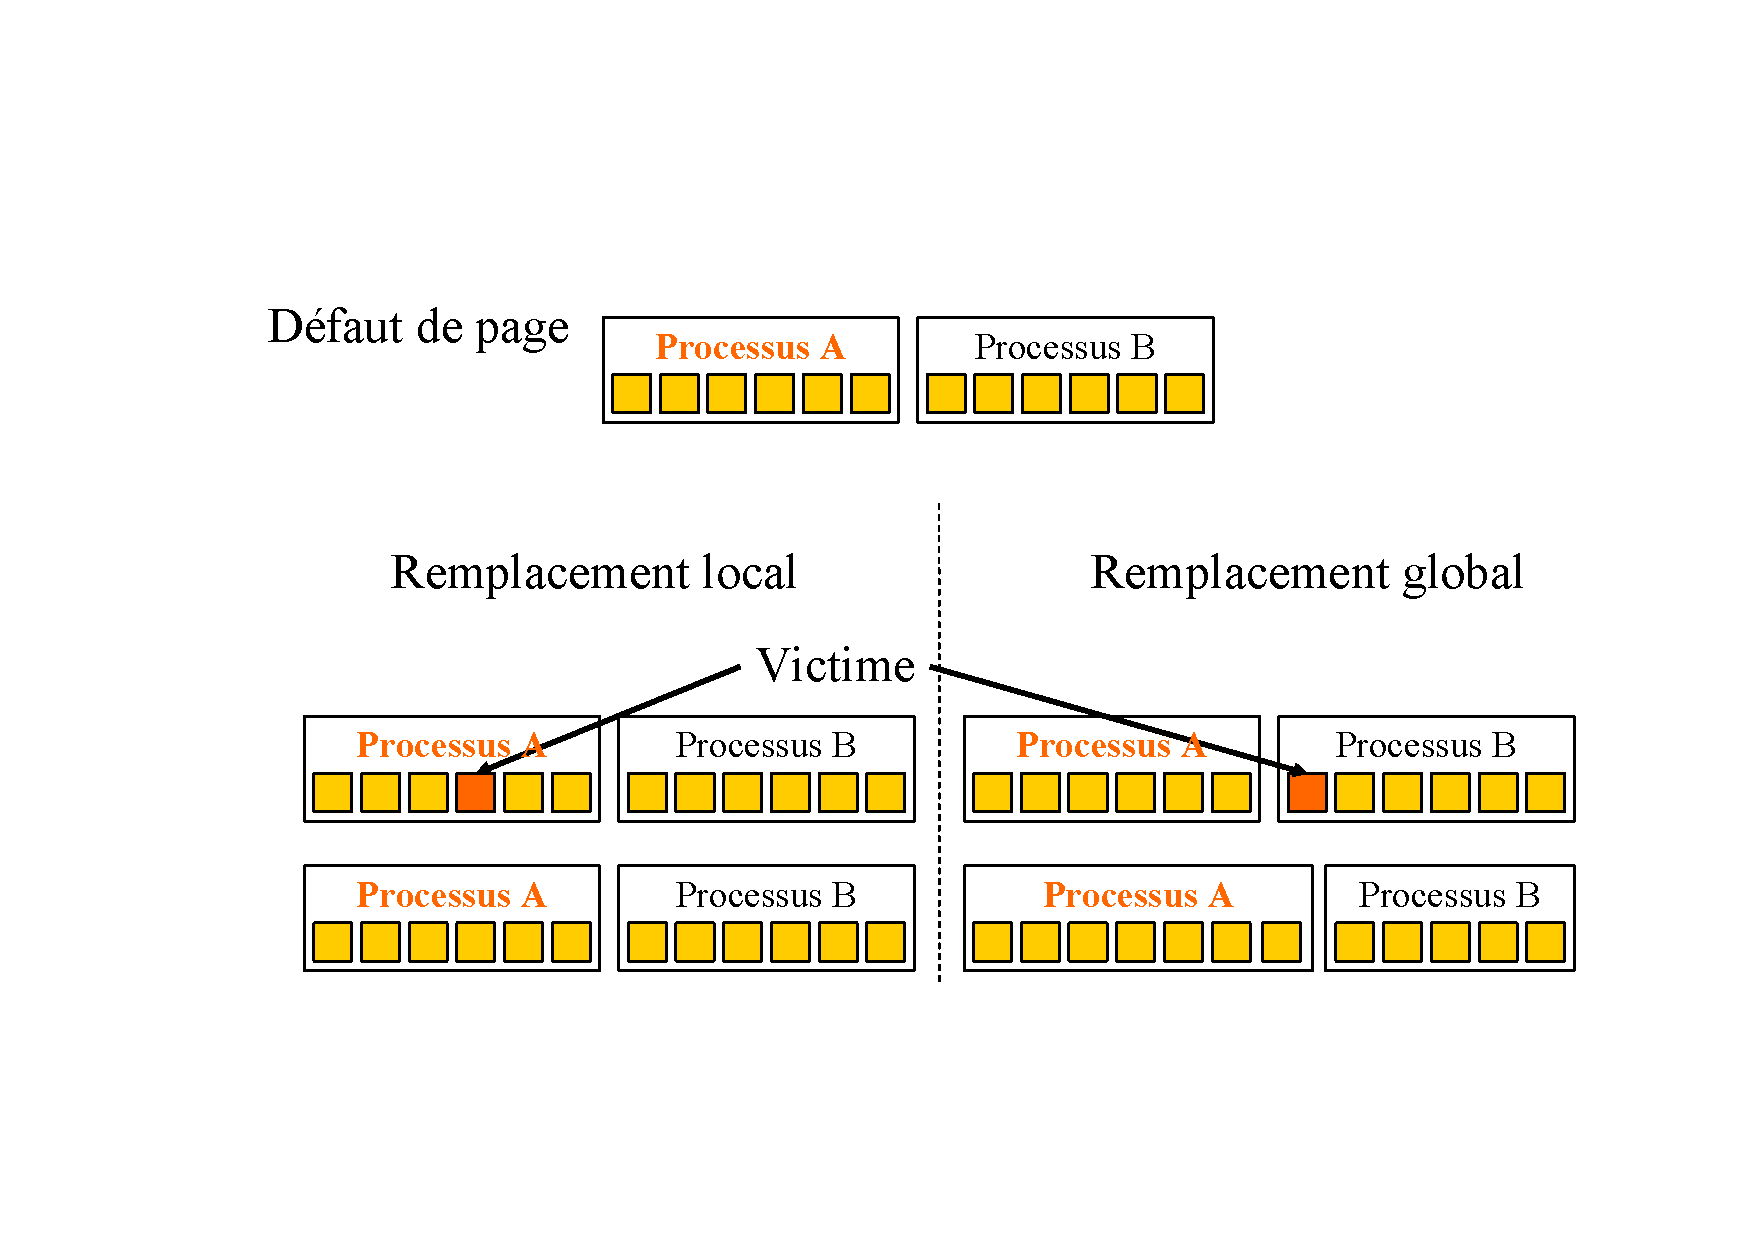
\includegraphics[width=.9\textwidth]{../illustration/remplacement_portee.pdf}
\end{frame}


\begin{frame}
\frametitle{Remplacement local ou global}
\begin{itemize}
\item Remplacement local :
\begin{itemize}
\item Taux de défaut de page contrôlé au niveau de chaque processus
\item Mauvaise utilisation de la mémoire
\item Contraignant
\end{itemize}
\item Remplacement global :
\begin{itemize}
\item Permet un débit plus important
\item Méthode la plus généralement utilisée
\item Moindre contrôle du taux de défaut de page
\end{itemize}
\end{itemize}
\end{frame}


\begin{frame}
\frametitle{Compromis entre remplacement local et global }
\begin{itemize}
\item Prise en compte de la priorité des processus
\item \textbf{Remplacement global} :
\begin{itemize}
\item Sur les processus de \textbf{priorité inférieure}
\end{itemize}
\item \textbf{Remplacement local} :
\begin{itemize}
\item Sur les processus de \textbf{priorité plus élevée}
\end{itemize}
\item Exécution plus rapide processus haute priorité (mais aussi risque de famine)
\end{itemize}
\end{frame}


\begin{frame}
\frametitle{Allocation de cadres de page}
\begin{itemize}
\item Comment allouer les cadres de pages disponibles aux différents processus concurrents ?
\item Besoins :
\begin{itemize}
\item Utilisation efficace des ressources disponibles
\item Répartition équitable des ressources
\item Cloisonnement inter-processus
\end{itemize}
\end{itemize}
\end{frame}


\begin{frame}
\frametitle{Nombre minimal de pages allouées}
\begin{itemize}
\item Diminution du nombre de pages allouées :
\begin{itemize}
\item Augmentation du nombre de défaut de page
\item Impossibilité de réaliser certaines opérations
\begin{itemize}
\item Les données doivent être présentes en mémoire
\end{itemize}
\end{itemize}
\item Nombre minimum de pages allouées :
\begin{itemize}
\item Nombre maximal de pages pouvant être manipulées par une instruction
\end{itemize}
\end{itemize}
\end{frame}


\begin{frame}
\frametitle{Influence du jeu d'instructions}
\begin{itemize}
\item Les pages utilisées par une instruction doivent nécessairement se trouver en mémoire lors de l'exécution
\begin{itemize}
\item Défaut de page dans le cas contraire (\textbf{interruption})
\item Reprise de l'exécution \textbf{au début} de l'instruction interrompue
\end{itemize}
\item Problème si le processus ne dispose pas d'assez de cadre de page pour stocker toutes les pages manipulées par une instruction
\begin{itemize}
\item Provoque des défauts de page en cascade
\item Blocage du système
\end{itemize}
\end{itemize}
\end{frame}


\begin{frame}
\frametitle{Nombre minimal de pages allouées}
\begin{itemize}
\item Exemple : Instruction de recopie mémoire 
\begin{itemize}
\item Recopie de la valeur située à une adresse vers un autre emplacement mémoire
\item Peut utiliser jusqu'à trois pages :
\begin{itemize}
\item Opération
\item Valeur à copier
\item Emplacement où copier la valeur
\end{itemize}
\end{itemize}
\item Impossible à réaliser si le processus ne dispose pas d'\textbf{au moins 3 cadres de pages}
\end{itemize}
\end{frame}


%\begin{frame}
%\frametitle{Nombre minimal de pages allouées}
%\begin{itemize}
%\item Indirection mémoire :
%\begin{itemize}
%\item Référence d’une page mémoire vers une autre
%\item Référence chaînée de pages
%\end{itemize}
%\item Niveau d'indirection :
%\begin{itemize}
%\item Niveau 0 : Pas d'indirection
%\item Niveau n : n indirections successives autorisées
%\end{itemize}
%\end{itemize}
%\end{frame}
%
%
%
%\begin{frame}
%\frametitle{Nombre minimal de pages allouées}
%\begin{itemize}
%\item Cas extrême :
%\begin{itemize}
%\item Référencer l'ensemble de la mémoire depuis une seule référence
%\end{itemize}
%\end{itemize}
%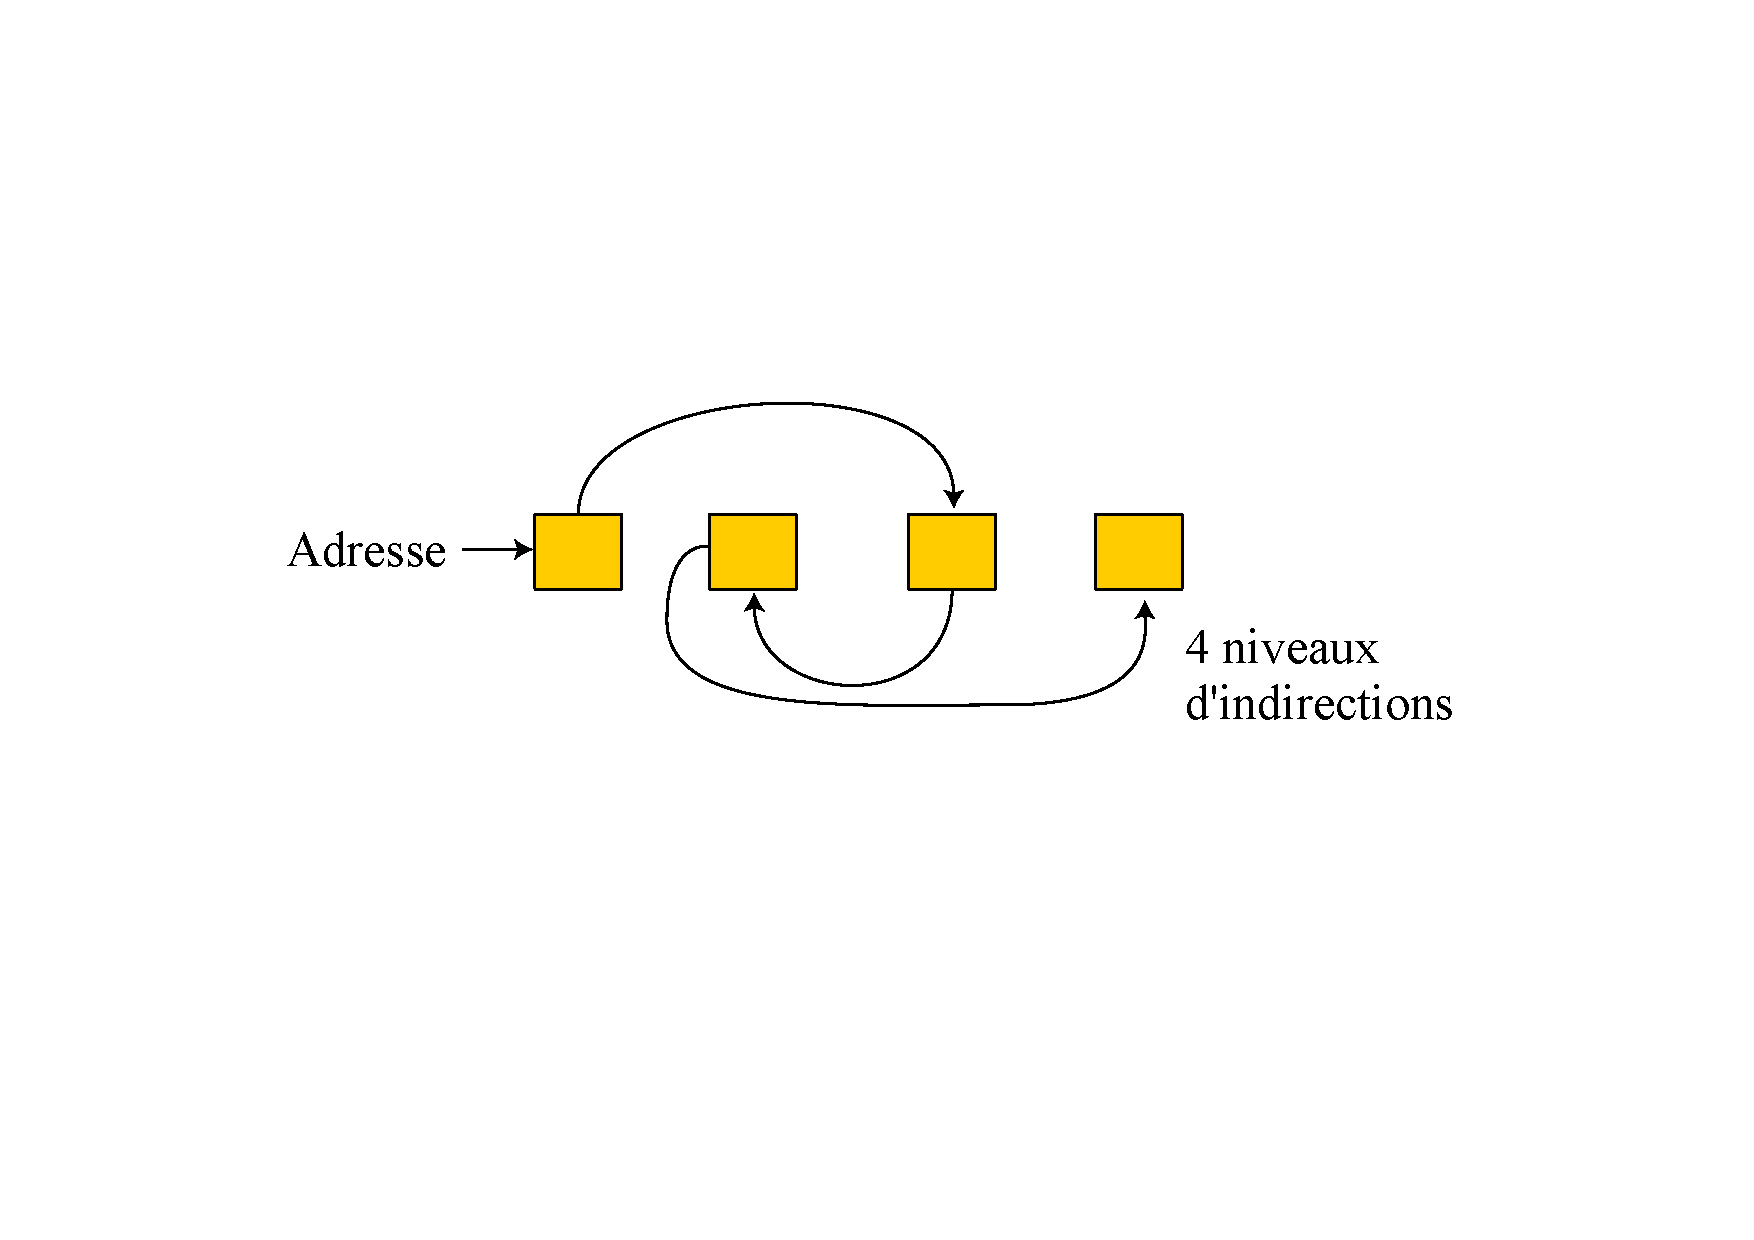
\includegraphics[width=.8\textwidth]{../illustration/indirection_memoire.pdf}
%\begin{itemize}
%\item Indirection mémoire :
%\begin{itemize}
%\item Instruction nécessite ensemble mémoire
%\item Limitation du niveau d'indirection (16 par exemple)
%\end{itemize}
%\end{itemize}
%\end{frame}


\begin{frame}
\frametitle{Nombre mini de pages allouées}
\begin{itemize}
\item Si le \textbf{nombre de cadres alloué} à un processus est inférieur au \textbf{nombre de cadres maximal requis} par le jeu d'instruction du processeur
\begin{itemize}
\item Il faut \textbf{suspendre} son activité
\item Sinon, il y a un \textbf{risque de blocage} définitif du système
\end{itemize}
\end{itemize}
\end{frame}


\begin{frame}
\frametitle{Algorithmes d'allocation de cadres}
\begin{itemize}
\item But :
\begin{itemize}
\item \textbf{Partager} les cadres disponibles entre les différents processus du système
\end{itemize}
\item Contraintes :
\begin{itemize}
\item \textbf{Répartir équitablement} la mémoire en fonction des besoins
\item \textbf{Éviter la monopolisation} de la mémoire par quelques processus au détriment des autres
\item \textbf{Optimiser} l'utilisation de la mémoire
\end{itemize}
\end{itemize}
\end{frame}


\begin{frame}
\frametitle{Algorithmes d'allocation de cadres}
Allocation à la \textbf{demande} :
\begin{itemize}
\item Pas de contrôle, allocation en fonction des demandes des processus
\item Risque de monopolisation de la mémoire par un processus
\item Augmente le nombre de défaut de page pour tous les autres processus du système
\end{itemize}
\end{frame}


\begin{frame}
\frametitle{Algorithmes d'allocation de cadre}
Allocation \textbf{équitable} :
\begin{itemize}
\item Méthode la plus simple
\item Répartir un nombre équitable de cadres pour chaque processus
\item Tous les processus sont sur un pied d'égalité
\item Ne tient pas compte de la disparité des travaux réalisés par le système
\begin{itemize}
\item Gaspillage de page pour les petits processus
\item Mauvaise utilisation des ressources pour les autres
\end{itemize}
\end{itemize}
\end{frame}

\begin{frame}
\frametitle{Algorithmes d'allocation de cadre}
Allocation \textbf{proportionnelle}
\begin{itemize}
\item Nombre de cadres alloué en fonction de la taille de la mémoire virtuelle du processus
\item Réquisition de cadres possible lors de l'augmentation du niveau de multiprogrammation
\item Gestion éventuelle des priorités de processus
\begin{itemize}
\item Comme unique critère d'attribution
\item Combiné avec la taille du processus
\end{itemize}
\end{itemize}
\end{frame}

\begin{frame}
\frametitle{Limites de la mémoire centrale}
\begin{itemize}
\item Dans l’idéal :
\begin{itemize}
\item Toutes les données et instructions résident en permanence dans la mémoire centrale
\end{itemize}
\item Impossible car :
\begin{itemize}
\item Mémoire centrale généralement trop petite
\item La mémoire centrale est volatile
\end{itemize}
\item Nécessité d’un stockage secondaire
\begin{itemize}
\item Peut maintenir une grande quantité de données de manière permanente
\end{itemize}
\end{itemize}
\end{frame}

%\subsection{Allocateurs SLAB/SLUB du noyau Linux}





%------------------------------------------------------------------- 
\section{Système de fichiers}
%------------------------------------------------------------------- 

\begin{frame}
\frametitle{Système de fichiers}
\begin{itemize}
\item Partie la plus ''visible'' d'un système pour les utilisateurs
\item Buts :
\begin{itemize}
\item Fournir les mécanismes fiables de \textbf{stockage des informations}
\begin{itemize}
\item Volume de données important
\item Perein (subsiste après un redémarrage du système)
\end{itemize}
\item Permettre l'\textbf{accès aux données} pour le système et ses utilisateurs
\end{itemize}
\end{itemize}
\end{frame}

%---------------------------------------------------
\subsection{Les périphériques de stockage secondaire}
%---------------------------------------------------

\begin{frame}
\frametitle{Les disques magnétiques}
\begin{itemize}
\item Dispositif de stockage secondaire
\item Utilisés comme extension de la mémoire centrale
\item Stockage programme et données
\begin{itemize}
\item Jusqu’à leur chargement en mémoire
\item Utilisé par de nombreux programmes en entrée ou sortie de traitement
\end{itemize}
\end{itemize}
\end{frame}

\begin{frame}
\frametitle{Disques magnétiques}
\begin{itemize}
\item Les informations ne peuvent pas être adressées depuis le processeur
\item Ces informations doivent être transférées en mémoire centrale pour pouvoir être utilisées par le processeur
\item Nécessite une requête d’E/S
\begin{itemize}
\item Accès au disque assuré par le contrôleur du périphérique
\end{itemize}
\end{itemize}
\end{frame}

\begin{frame}
\frametitle{Disques magnétiques}
Périphérique « mécanique »
\begin{itemize}
\item Plateaux magnétiques circulaires
\begin{itemize}
\item Divisés en pistes/secteurs
\item En rotation autour d ’un axe
\end{itemize}
\item Bras de disque
\begin{itemize}
\item Supporte les têtes de lecture/écriture
\item Déplacement latéral
\end{itemize}
\item Tête de lecture/écriture en survol
\end{itemize}
\end{frame}

\begin{frame}
\frametitle{Disques magnétiques}
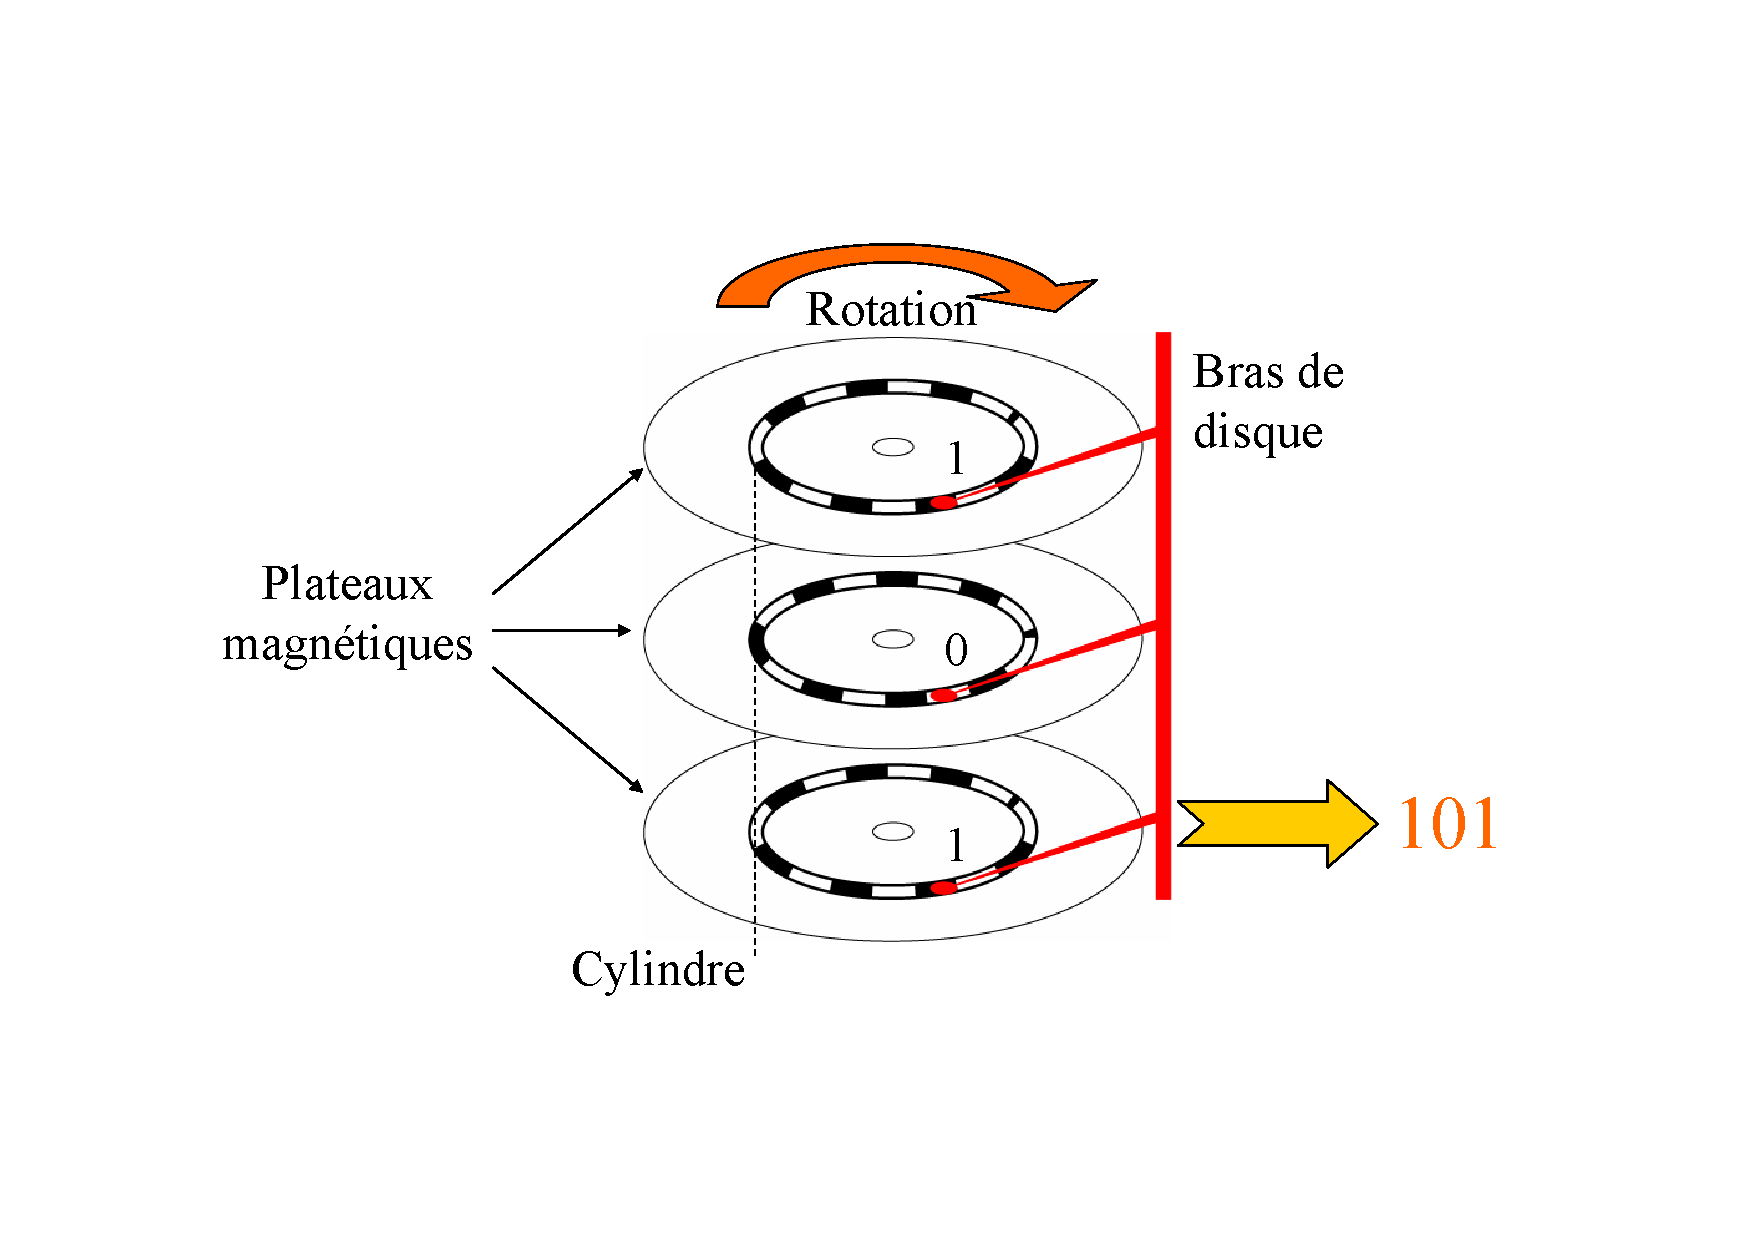
\includegraphics[height=6cm]{../illustration/decomp_hd.pdf}
\end{frame}

\begin{frame}
\frametitle{Disques magnétiques}
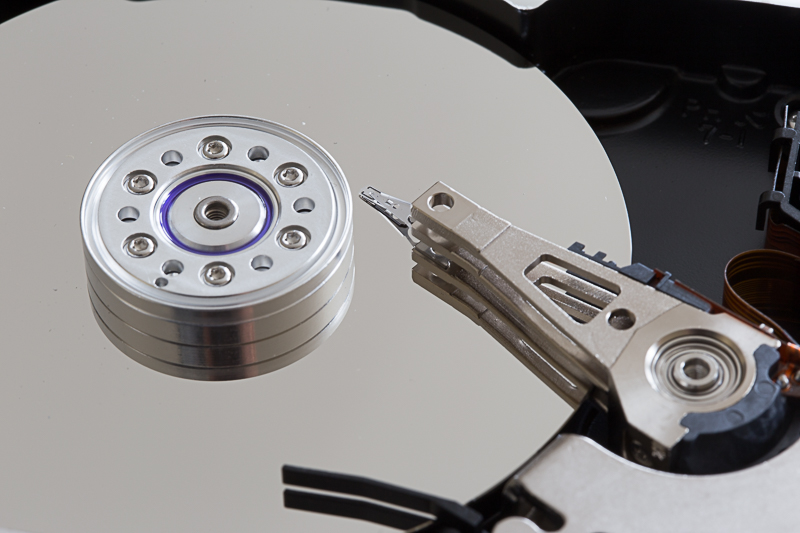
\includegraphics[height=6cm]{../illustration/disque_dur.jpg}
\end{frame}

\begin{frame}
\frametitle{Performances des disques magnétiques}
\begin{itemize}
\item Taux de transfert
\begin{itemize}
\item Vitesse de passage des données du disque à la mémoire centrale
\end{itemize}
\item Temps de positionnement
\begin{itemize}
\item Temps aléatoire
\begin{itemize}
\item Variable en fonction de la position courante du disque
\end{itemize}

\item Temps de recherche : 
\begin{itemize}
\item Positionnement du bras sur le cylindre recherché
\end{itemize}
\item Latence de rotation :
\begin{itemize}
\item Positionnement de la tête sur le secteur recherché
\end{itemize}
\end{itemize}
\end{itemize}
\end{frame}

\begin{frame}
\frametitle{Disques magnétiques amovibles}
\begin{itemize}
\item Disquette, Zip...
\begin{itemize}
\item Un seul disque souple
\item Contact tête - disque
\item Vitesse de rotation faible
\end{itemize}
\item Disque dur amovible
\begin{itemize}
\item Comparable aux disques durs fixes
\item Performances moindres, pour assurer la fiabilité
\end{itemize}
\end{itemize}
\end{frame}


\begin{frame}
\frametitle{Les disques SSD}
\begin{itemize}
\item Solid State Drive
\begin{itemize}
\item lecteur à l'état solide
\item aucune pièce en mouvement
\end{itemize}

\item Mémoire flash
\begin{itemize}
\item Caractéristiques d'une mémoire vive (accès aléatoire)
\item Pérennité des données après mise hors tension (EEPROM)
\end{itemize}
\end{itemize}
\end{frame}


\begin{frame}
\frametitle{Les disques SSD}
Deux principales technologies :
\begin{itemize}
\item \textbf{NOR}
\begin{itemize}
\item Inventée par Intel en 1988
\item Écriture lente, lecture rapide et fiable (100\%)
\item Densité faible et coût élevé
\end{itemize}
\item \textbf{NAND}
\begin{itemize}
\item Développée par Toshiba en 1989
\item Plus rapide à l'effacement et à l'écriture
\item Densité importante et faible coût
\item Peu fiable (vérification et répartition des écritures - mise en place d'EEC -\begin{tiny} Error Code Correction\end{tiny})
\item Limite la vitesse de lecture
\end{itemize}
\end{itemize}
\end{frame}

\begin{frame}
\frametitle{La mémoire NAND}
\begin{center}
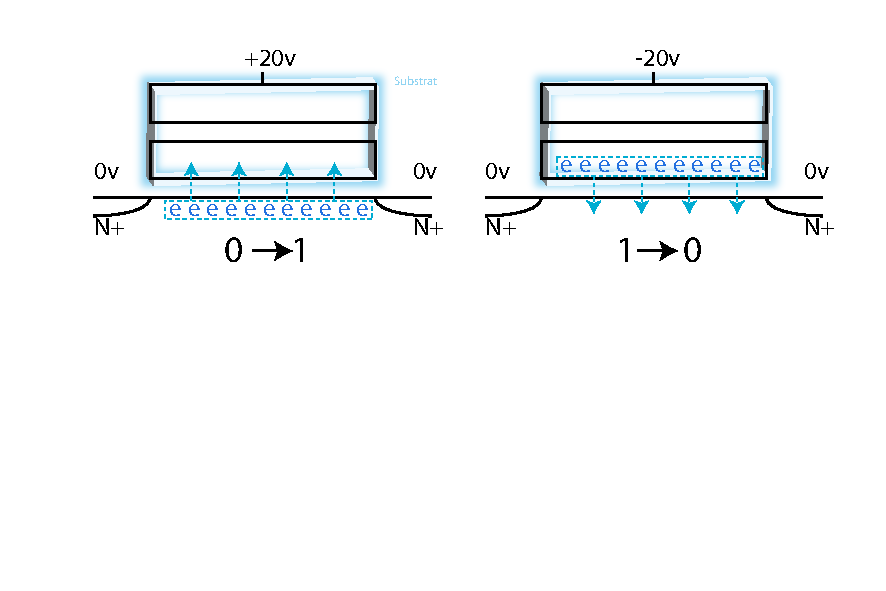
\includegraphics[width=10cm]{../illustration/NAND_modif.pdf}
\end{center}
\end{frame}

\begin{frame}
\frametitle{La mémoire NAND}
Deux types de mémoire NAND :
\begin{itemize}
\item SLC (Single Level Cell)
\begin{itemize}
\item stocke un seul bit dans chaque cellule (deux niveaux de charge)
\end{itemize}
\item MLC (Multi Level Cell)
\begin{itemize}
\item stocke plusieurs bits dans la même cellule
\item le plus souvent 2 bits (quatre niveaux de charge)
\end{itemize}
\item TLC (Triple Level Cell)
\begin{itemize}
\item 3 bits par cellule (huit niveaux de charge)
\end{itemize}
\end{itemize}
\end{frame}

\begin{frame}
\frametitle{Performances des différentes mémoire NAND}
\begin{itemize}
\item MLC et TLC moins coûteux à produire
\begin{itemize}
\item SSD bas de gamme
\end{itemize}

\item Mais dégrade les performances, surtout en écriture
\item Réduit grandement la durée de vie des cellules.
\end{itemize}

\begin{table}[htdp]
\caption{Nombre de cycles écriture/effacement des différents types de mémoire NAND}
\begin{center}
\begin{tabular}{c|c}
Type de mémoire & Durée de vie \\
\hline
SLC & 100 000 cycles par cellule \\
MLC &  3 000 à 10 000 cycles par cellule \\
TLC & 1 000 cycles par cellule \\
\end{tabular}
\end{center}
\label{default}
\end{table}
\textit{Disques SSD de production $\rightarrow$ mémoire SLC.}
\end{frame}

\begin{frame}
\frametitle{À venir... technologie 3D XPoint ("CrossPoint") \cite{XPoint}}
\begin{itemize}
\item Collaboration entre Intel et Micron Technology
\item Amélioration des performances de la SSD (annoncée)
\begin{itemize}
\item Vitesse : 
\begin{itemize}
\item 1000 fois plus rapide\footnote{Que la mémoire NAND}
\item Latence de l'ordre de la nanoseconde\footnote{Microseconde pour les SSD, milliseconde pour un HDD}
\end{itemize}

\item Durée de vie : 1000 fois plus endurante
\item Capacité : 10 fois plus dense
\end{itemize}
\item Transistors $\rightarrow$  points de croisement (empilement)
\end{itemize}

\begin{figure}[htbp]
\begin{center}
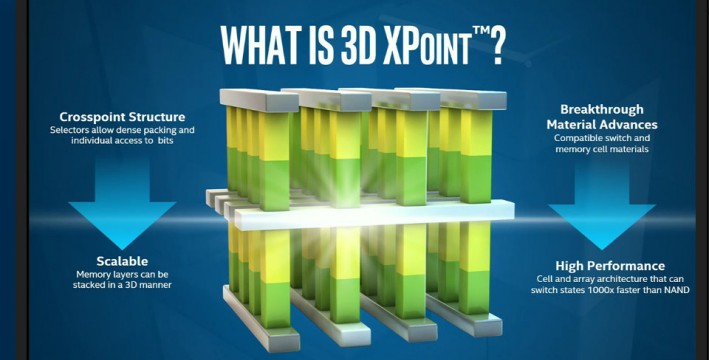
\includegraphics[height=2.5cm]{../illustration/XPoint.jpg}
\label{default}
\end{center}
\end{figure}

\end{frame}

\begin{frame}
\frametitle{Mémoire SSD - la commande TRIM}
\begin{itemize}

\item Amplification d’écriture (\textit{write amplification})
\begin{itemize}
\item Manipulation de blocs de 4ko
\item Effacement préalablement de blocs plus larges (128 ou 512 ko)
\item Cycle lecture-effacement-modification-écriture
\end{itemize}

\item TRIM : optimisation SSD par le système
\begin{itemize}
\item Informe le contrôleur des blocs contenant des données
\item Identification des blocs effacés
\end{itemize}

\item Mise à niveau de l’usure (\textit{wear levelling})
\begin{itemize}
\item Réarrangement des données
\begin{itemize}
\item répartition des écritures sur les différentes cellules
\end{itemize}

\item Déplacement des données 
\item Nécessite de connaître les blocs utilisés ou non
\end{itemize}

\end{itemize}

\end{frame}

\begin{frame}
\frametitle{Bandes magnétiques}
\begin{itemize}
\item Grande capacité
\item Temps d’accès longs
\item Taux de transfert élevés
\item Économiques
\item Encore utilisées pour :
\begin{itemize}
\item Sauvegarde
\item Archivage
\item Transferts
\end{itemize}
\end{itemize}
\end{frame}

\begin{frame}
\frametitle{Les bandes magnétiques}
\begin{center}
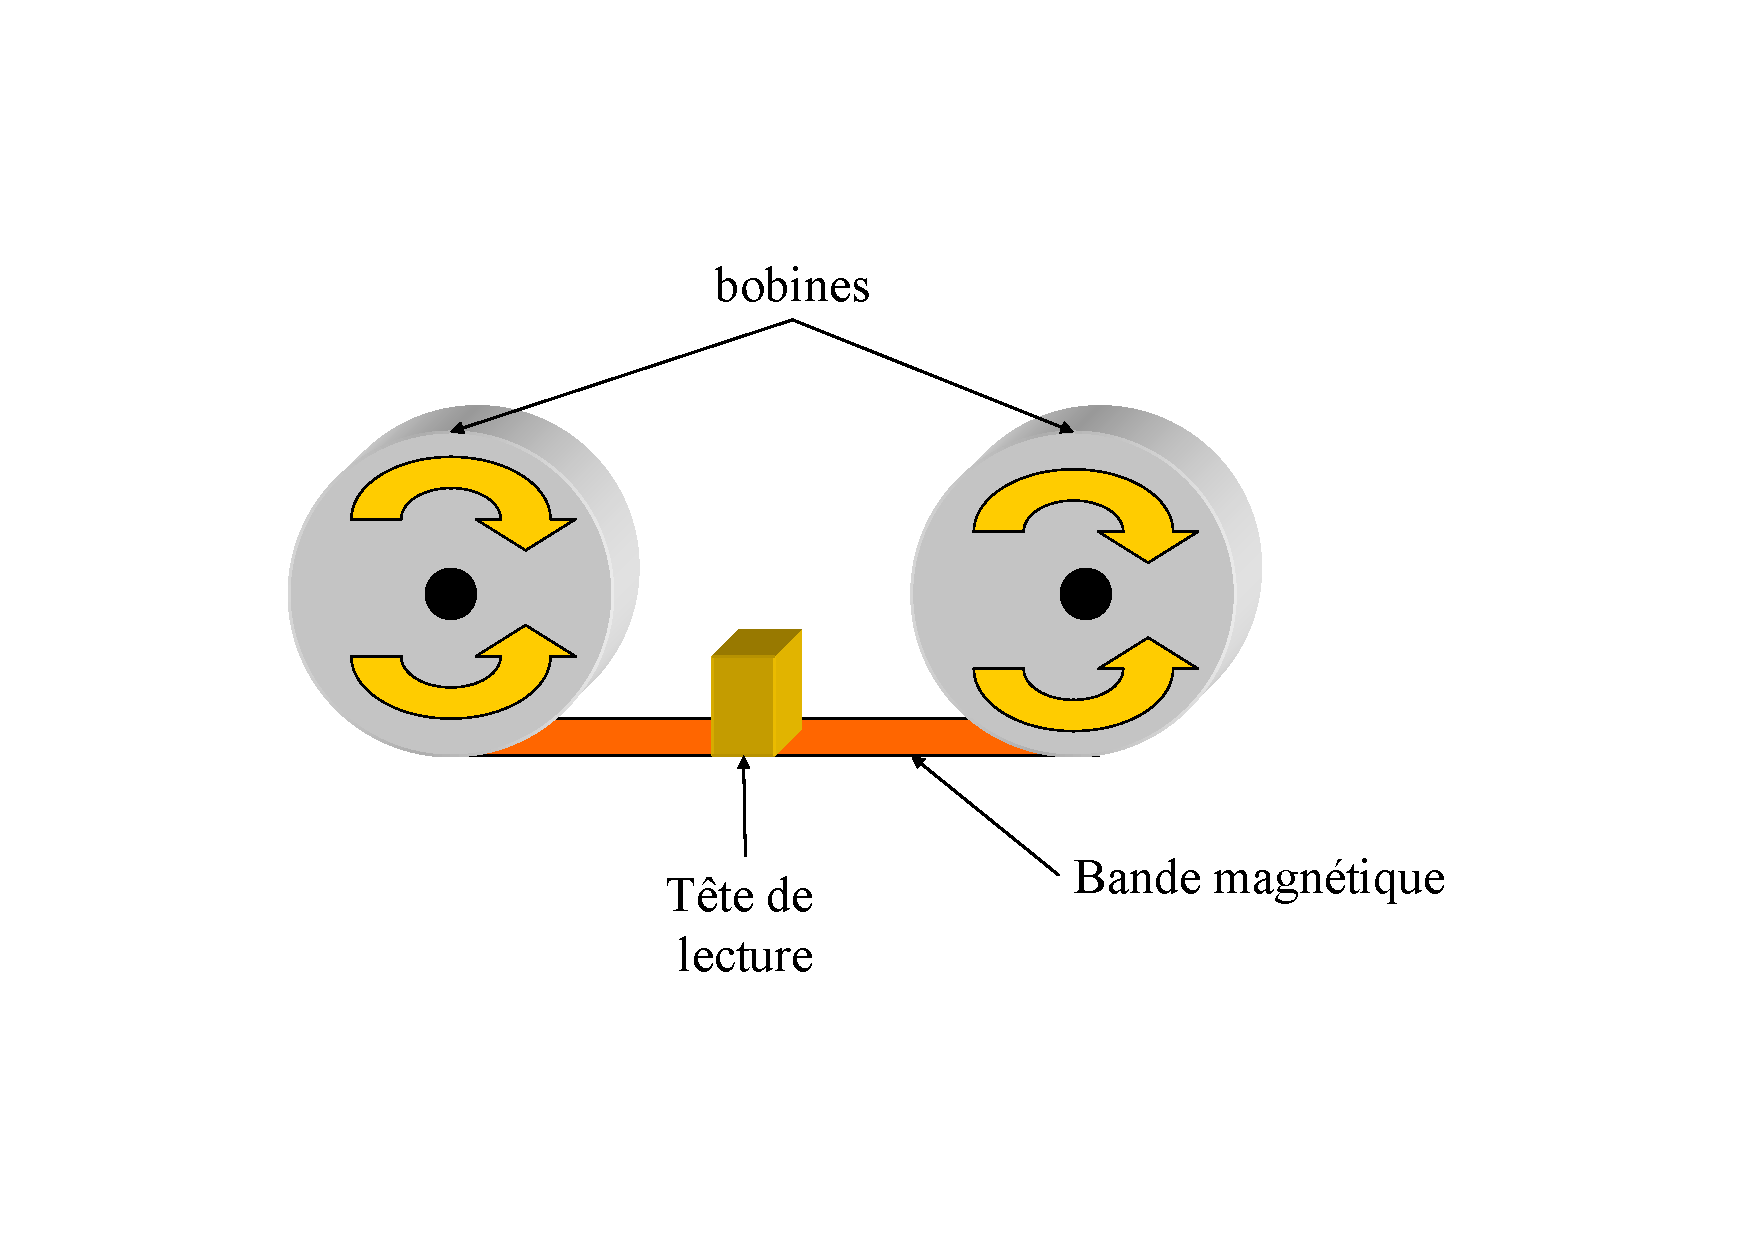
\includegraphics[height=0.8\textheight]{../illustration/bande.pdf}
\end{center}
\end{frame}


\begin{frame}
\frametitle{La technologie RAID}
\begin{itemize}
\item Redundant Array of Inexpensive Disks
\item Constituer une \textbf{unité de stockage} à partir de \textbf{plusieurs disques} (grappe)
\item Une \textbf{grappe} peut offrir :
\begin{itemize}
\item Plus grande \textbf{tolérance aux pannes}
\item Plus grande \textbf{capacité d'écriture}
\item Meilleurs \textbf{performances}
\end{itemize}
\end{itemize}
\end{frame}

\begin{frame}
\frametitle{Plusieurs niveaux RAID}
\begin{tabular}{c|l}
\textbf{RAID 0} & Entrelacement (Striping) \\
\textbf{RAID 1} & Miroir (Mirroring, shadowing, duplexing) \\
\textbf{RAID 3} & Disk array with bit-interleaved data \\
\textbf{RAID 4} & Disk array with block-interleaved data \\
\textbf{RAID 5} & Disk array with block-interleaved distributed parity \\
\end{tabular}
\end{frame}


\begin{frame}
\frametitle{RAID 0}
\begin{columns}
\column{.6\textwidth}
\begin{itemize}
\item \textbf{Chaînage} de disques
\item Les disques peuvent être différents
\item \textbf{Entrelacement} des données
\item Agrégats par bandes
\end{itemize}
\begin{itemize}
\item Augmente la \textbf{capacité}
\item Améliore le \textbf{taux de transfert}
\item Dégrade la \textbf{fiabilité}
\end{itemize}
\column{.4\textwidth}
\includegraphics[width=4cm]{../illustration/RAID0.pdf}
\end{columns}
\end{frame}


\begin{frame}
\frametitle{RAID 1}
\begin{columns}
\column{.5\textwidth}
\begin{itemize}
\item \textbf{Miroir}
\item Recopie des données à l'identique sur deux disques
\end{itemize}
\begin{itemize}
\item \textbf{Sécurité}
\item Amélioration des \textbf{performances en lecture}
\item Gaspillage de la moitié de l’espace disque
\end{itemize}
\column{.5\textwidth}
\includegraphics[height=4cm]{../illustration/RAID1.pdf}
\end{columns}
\end{frame}


\begin{frame}
\frametitle{RAID 3}
\begin{columns}
\column{.5\textwidth}
\begin{itemize}
\item Disques identiques
\item \textbf{Parité bit à bit}
\end{itemize}
\begin{itemize}
\item Sécurité
\item Utilisation des 2/3 de l’espace disque
\end{itemize}
\column{.5\textwidth}
\includegraphics[height=4cm]{../illustration/RAID3.pdf}
\end{columns}
\end{frame}


\begin{frame}
\frametitle{RAID 5}
\begin{columns}
\column{.5\textwidth}
\begin{itemize}
\item N disques (au moins 3)
\item Parité répartie sur l’ensemble des disques
\end{itemize}
\begin{itemize}
\item Sécurité
\item Utilisation des (n-1)/n de l’espace disque
\item Performances
\end{itemize}
\column{.5\textwidth}
\includegraphics[height=4cm]{../illustration/RAID5.png}
\end{columns}
\end{frame}


\begin{frame}
\frametitle{La technologie RAID}
\begin{itemize}
\item Trois critères de choix :
\begin{itemize}
\item La sécurité
\item Les performances
\item Le coût
\end{itemize}
\item Pris en charge par :
\begin{itemize}
\item Logiciel : Drivers
\item Matériel : Contrôleurs ou DASD
\end{itemize}
\end{itemize}
\end{frame}

\begin{frame}
\frametitle{La technologie RAID}
\begin{tabular}{c|*{2}{p{4cm}|}}
 & Avantages & Inconvénients \\
\hline
\textbf{Raid 0} & \begin{small}Performances en lecture / écriture\end{small} & \begin{small}Pas de tolérance aux pannes\end{small} \\
 & Capacité & \\
\hline
\textbf{Raid 1} & \begin{small}Performances en lecture\end{small} & \begin{small}Perte de capacité de 50\%\end{small} \\
 & \begin{small}Tolérance aux pannes\end{small} & \\
 & \begin{small}Temps de reprise sur panne\end{small} & \\
\hline
\textbf{Raid 3} & \begin{small}Optimisation de la capacité\end{small} & \begin{small}Performances\end{small} \\
 & \begin{small}Tolérance aux pannes\end{small} & \begin{small}(disque de parité)\end{small} \\
\hline
\textbf{Raid 5} & \begin{small}Souplesse\end{small} & \begin{small}Coût de reconstruction\end{small} \\
 & \begin{small}Performance\end{small} & \\
\end{tabular}
\end{frame}


%-----------------------------------------------
\subsection{Concept de fichier}
%-----------------------------------------------

\begin{frame}
\frametitle{Composantes du système de fichiers}
Deux parties distinctes :
\begin{itemize}
\item \textbf{Collection} de fichiers :
\begin{itemize}
\item \textbf{Stockage} de l'information
\item Sur le dispositif de stockage
\end{itemize}
\item \textbf{Structure} de répertoire : 
\begin{itemize}
\item \textbf{Organisation} des informations stockées
\item Permet de retrouver les données stockées
\end{itemize}
\end{itemize}
\end{frame}


\begin{frame}
\frametitle{Concept de fichier}
\begin{itemize}
\item Stockage des informations sur \textbf{supports variés} :
\begin{itemize}
\item Disques magnétiques,
\item Bandes magnétiques,
\item Disques optiques...
\end{itemize}
\item Nécessité de disposer d'une \textbf{vue logique} des ces systèmes de stockage
\begin{itemize}
\item Indépendante du support utilisé
\item Abstraction du mode de stockage physique
\item Mêmes méthodes d'accès
\end{itemize}
\end{itemize}
\end{frame}

\begin{frame}
\frametitle{Concept de fichier}
\begin{itemize}
\item Fichier :
\begin{itemize}
\item \textbf{Vue logique} uniforme du stockage fournie par le système
\item Permet de faire \textbf{abstraction} du dispositif utilisé pour stocker les informations
\item \textbf{Collection nommée} d'informations apparentées
\item Entité manipulée par l'utilisateur d'un système de fichier
\end{itemize}
\end{itemize}
\includegraphics[scale=.5]{../illustration/fichier.png} 
\end{frame}

\begin{frame}
\frametitle{Concept de fichier}
\begin{itemize}
\item Enregistré sur un support de \textbf{mémoire secondaire}
\item Pour l'utilisateur :
\begin{itemize}
\item Le fichier est la plus petite \textbf{unité logique d'allocation} de mémoire secondaire
\item Toutes les données écrites en mémoire secondaire doivent \textbf{résider dans un fichier}
\end{itemize}
\end{itemize}
\end{frame}

\begin{frame}
\frametitle{Contenu des fichiers}
\begin{itemize}
\item Le fichier peut représenter :
\begin{itemize}
\item Des \textbf{programmes}
\begin{itemize}
\item format source
\item format objet
\end{itemize}
\item Des \textbf{données}
\begin{itemize}
\item Format numérique
\item Format alphanumérique
\item Format binaire
\item Format quelconque ou strict
\item Signification définie par le créateur du fichier
\end{itemize}
\end{itemize}
\end{itemize}
\end{frame}


\begin{frame}
\frametitle{Structure du contenu des fichiers}
Un fichier possède une \textbf{structure} définie par son \textbf{type}
\begin{itemize}
\item Fichier \textbf{texte} : 
\begin{itemize}
\item Succession de caractères organisée en lignes
\end{itemize}
\item Fichier \textbf{source} :
\begin{itemize}
\item Succession de commandes conformes à un langage de programmation
\end{itemize}
\item Fichier \textbf{objet} :
\begin{itemize}
\item Succession de commandes compréhensibles par un chargeur
\end{itemize}
\end{itemize}
\end{frame}


\begin{frame}
\frametitle{Attributs des fichiers}
Renseigne l'utilisateur et le système sur le \textbf{contenu} et \textbf{l'usage} du fichier

Métadonnées les plus courantes :
\begin{itemize}
\item Nom : identifiant
\item Type : qualification du contenu (strict ou indicatif)
\item Emplacement
\item Taille : en octet, blocs
\item Dates : de création, de modification, d'accès
\item Protection, identification des utilisateurs
\end{itemize}
\end{frame}


\begin{frame}
\frametitle{Typage de fichier}
\begin{itemize}
\item \textbf{Qualification} du \textbf{contenu} du fichier
\begin{itemize}
\item Permet de connaître les \textbf{opérations valides}
\item Pris en charge par certains systèmes
\end{itemize}
\item Techniques courantes :
\begin{itemize}
\item Inclure le type dans le nom (extensions)
\item Attribut "\texttt{type}" du fichier (+ nom du programme créateur)
\item Nombre magique stocké en début de fichier
\end{itemize}
\end{itemize}
\end{frame}

\begin{frame}
\frametitle{Exemple de typage : \textbf{MacOs}}
\begin{itemize}
\item Chaque fichier possède les attributs suivants :
\begin{itemize}
\item Type : Exemple "\texttt{pict}", "\texttt{text}"…
\item Nom du programme ayant créé le fichier
\end{itemize}
\item Positionnés par le système lors de la création du fichier
\item Géré par le système
\end{itemize}
\includegraphics[width=1cm]{../illustration/logo_macos.png}
\end{frame}

\begin{frame}
\frametitle{Exemple de typage : \textbf{Unix}}
\begin{itemize}
\item Nombre magique stocké au début de certains fichiers
\item Indique grossièrement le type du fichier :
\begin{itemize}
\item Fichier exécutable,
\item Script (nom de l'interpréteur),
\item Fichier texte,
\item Fichier PostScript…
\end{itemize}
\item Simulation des extensions de fichier lors du nommage
\end{itemize}
\includegraphics[width=1cm]{../illustration/logo_tux.png}
\end{frame}

\begin{frame}
\frametitle{Structure des fichiers}
\begin{itemize}
\item Correspondance entre type de fichier et structure interne :
\begin{itemize}
\item Fichier exécutable
\item Fichier source...
\end{itemize}
\item Prise en charge par le système possible
\begin{itemize}
\item Utilisation du type de fichier
\item Instructions de manipulation dédiées
\end{itemize}
\end{itemize}
\begin{exampleblock}{VMS de DEC}
3 structures de fichier :
\begin{itemize}
\item Exécutable
\item Texte
\item Séquentiel indexé
\end{itemize}
\end{exampleblock}
\end{frame}

\begin{frame}
\frametitle{Gestion avancé des structures des fichiers}
\begin{columns}
\column{0.5\textwidth}
\begin{block}{Avantages}
\begin{itemize}
\item Support avancé
\item Haut niveau d'abstraction
\item Optimisation des performances
\end{itemize}
\end{block}
\column{0.5\textwidth}
\begin{block}{Inconvénients}
\begin{itemize}
\item Complexification de l'OS
\begin{itemize}
\item Code propre à chaque type de fichier
\end{itemize}
\item Rigidification de l'OS
\begin{itemize}
\item nouveaux types de fichiers 
\end{itemize}
\end{itemize}
\end{block}
\end{columns}
\end{frame}

\begin{frame}
\frametitle{Gestion d'un minimum de types de fichier}
\begin{itemize}
\item Fichier = \textbf{séquence d'octets}
\begin{itemize}
\item Pas d'interprétation du contenu des fichiers
\end{itemize}
\item Souplesse maximale
\item Support dérisoire
\begin{itemize}
\item Développement des outils de manipulation des données pour chaque applicatif
\item Au moins une structure gérée :
\begin{itemize}
\item Fichiers exécutables (chargement)
\end{itemize}
\end{itemize}
\end{itemize}
\end{frame}

\begin{frame}
\frametitle{Exemple de structure des fichiers : \textbf{MacOS}}
\begin{itemize}
\item Fichier composé de deux parties :
\begin{itemize}
\item Branche de \textbf{ressources}
\begin{itemize}
\item Ressources utilisées (\textit{libellés des boutons, traduction des menus, icônes, fichiers son, emplacement fenêtre… })
\item Possibilité de paramétrer facilement la langue utilisée
\end{itemize}
\item Branche de \textbf{données}
\begin{itemize}
\item Contient les données ou le code exécutable
\end{itemize}
\end{itemize}
\item Facilite la vie du programmeur
\item Facilite la maintenance 
\end{itemize}
\includegraphics[width=1cm]{../illustration/logo_macos.png}
\end{frame}

\begin{frame}
\frametitle{Structure interne des fichiers}
\begin{itemize}
\item Fichier stocké sur disque
\item Information stockée sous forme de blocs :
\begin{itemize}
\item de taille fixe dans la plupart des cas (512 octets...)
\item de taille variable dans certains cas (ZFS - 512 o $\rightarrow$ 128 ko)
\end{itemize}
\item Fichier : Ensemble de blocs \textit{(au moins un)}
\begin{itemize}
\item Pas de correspondance enregistrement logique $\leftrightarrow$ bloc physique
\item Regroupe plusieurs enregistrements logiques dans un bloc \textit{(ou inversement)}
\end{itemize}
\end{itemize}
\end{frame}

\begin{frame}
\frametitle{Structure interne des fichiers : Exemple d'Unix}
\begin{itemize}
\item Fichier = \textbf{flux d'octets}
\item Chaque octet est adressable individuellement
\begin{itemize}
\item Déplacement à partir du début (ou de la fin) du fichier
\end{itemize}
\item Le système se charge de compacter / décompacter les octets en blocs physiques
\begin{itemize}
\item 512 octets par bloc, par exemple
\end{itemize}
\item Fragmentation interne (sur dernier bloc)
\item \textbf{Support dérisoire}, mais usage \textbf{universel}
\end{itemize}
\includegraphics[width=1cm]{../illustration/logo_tux.png}
\end{frame}

\begin{frame}
\frametitle{Structure interne des fichiers : Exemple de VMS}
Fichier séquentiel indexé :
\begin{itemize}
\item Structure de fichier supportée nativement par certains systèmes
\begin{itemize}
\item VMS, MVS (OS/3090, 360... )
\end{itemize}
\item Permet un accès direct ou séquentiel aux données (annuaire)
\begin{itemize}
\item Massivement utilisé avant la généralisation des bases de données
\end{itemize}
\item \textbf{Support avancé}, mais rendu presque \textbf{obsolète} aujourd'hui...
\end{itemize}
\end{frame}


\begin{frame}
\frametitle{Attribut de protection}
\begin{itemize}
\item \textbf{Protection}
\begin{itemize}
\item Permet de définir les droits d'accès au fichier
\item Lecture
\item Écriture
\item Exécution
\item Suppression...
\end{itemize}
\end{itemize}
\end{frame}


\begin{frame}
\frametitle{Attributs d'affectation}
\begin{itemize}
\item \textbf{Identification des utilisateurs} :
\begin{itemize}
\item Identifiant de l'utilisateur ayant créé le fichier (propriétaire du processus créateur)
\item Identification des utilisateurs du fichier (ou du dernier utilisateur)
\end{itemize}
\item Permet de contrôler la protection des fichiers
\item Permet de vérifier l'utilisation des fichiers
\end{itemize}
\end{frame}


\begin{frame}
\frametitle{Contrôle d'accès aux données}
\begin{itemize}
\item Nécessaire dans le cas de systèmes multi-utilisateurs
\item Type d'accès :
\begin{itemize}
\item [Lecture] Lecture du contenu d'un fichier
\item [Écriture] Modification du contenu
\item [Exécution] Chargement fichier et exécution
\item [Ajout] Ajout de données en fin de fichier
\item [Destruction] Suppression du fichier
\item [Liste] Consultation des attributs du fichier
\end{itemize}
\end{itemize}
\end{frame}

\begin{frame}
\frametitle{Liste d'accès au fichier (ACL)}
\begin{itemize}
\item Possibilité de définir les droits individuellement, pour chaque utilisateur du système
\begin{itemize}
\item Définition de listes d'accès pour chaque fichier ou répertoire
\end{itemize}
\item Problèmes :
\begin{itemize}
\item taille des listes d'accès
\item définition et maintenance fastidieuses
\item taille de l'entrée de répertoire (importante et variable en fonction de la liste d'accès)
\end{itemize}
\end{itemize}
\end{frame}

\begin{frame}
\frametitle{Contrôle par classe}
\begin{itemize}
\item Chaque utilisateur est identifié
\item Il fait partie d'au moins un groupe
\item Classes d'utilisateurs (exemple UGO d'Unix) :
\begin{itemize}
\item [Propriétaire] Utilisateur ayant créé le fichier
\item [Groupe] Ensemble d'utilisateurs ayant besoin du fichier
\item [Univers] Tous les (autres) utilisateurs du système
\end{itemize}
\end{itemize}
\end{frame}

\begin{frame}
\frametitle{Contrôle par classe (Unix)}
\begin{itemize}
\item Définition des droits d'accès pour chaque classe d'utilisateurs
\begin{itemize}
\item Un champ pour chaque classe d'utilisateurs
\begin{tabular}{c|c|c|c|c}
& \textit{Lecture} & \textit{Ecriture} & \textit{Exécution} &  \\ 
\hline
Propriétaire & 1 & 1 & 1 & \textit{7} \\ 
Groupe & 1 & 0 & 1 & \textit{5} \\ 
Autres & 0 & 0 & 0 & \textit{0} \\  
\end{tabular} 
\end{itemize}
\end{itemize}
\end{frame}



\begin{frame}
\frametitle{Stockage des attributs de fichiers}
\begin{itemize}
\item Stockés dans la structure des répertoires
\begin{itemize}
\item De 16 à 1000 octets par fichier
\end{itemize}
\item Réside dans la mémoire secondaire
\item Chargés en mémoire principale lors de l'utilisation des fichiers
\begin{itemize}
\item Importance des mécanismes de cache sur les performances
\end{itemize}
\end{itemize}
\end{frame}


\begin{frame}
\frametitle{Opérations sur les fichiers}
\begin{itemize}
\item Permet d'accéder au contenu des fichiers
\item Réalisés par des appels système
\item Opérations de base :
\begin{itemize}
\item \textbf{Création} d'un fichier
\item \textbf{Écriture} dans un fichier
\item \textbf{Lecture} d'un fichier
\item \textbf{Repositionnement} dans un fichier
\item \textbf{Suppression} d'un fichier
\item \textbf{Troncature} d'un fichier
\end{itemize}
\end{itemize}
\end{frame}


\begin{frame}
\frametitle{Opération de création d'un fichier}
\begin{itemize}
\item Allocation de l'espace nécessaire sur le périphérique de stockage (dans le système de fichier)
\item Création d'une nouvelle entrée dans le répertoire
\begin{itemize}
\item Nom du fichier
\item Emplacement dans le système de fichier
\item Autres attributs...
\end{itemize}
\end{itemize}
\end{frame}


\begin{frame}
\frametitle{Opération d'écriture dans un fichier }
\begin{itemize}
\item Indication du nom du fichier et des informations à y écrire
\item Recherche du fichier dans le répertoire
\item Ouverture du fichier 
\item Attribution par le système d'un pointeur d'écriture (emplacement dans le fichier de la prochaine écriture)
\item Écriture des données
\end{itemize}
\end{frame}

\begin{frame}
\frametitle{Opération de lecture du contenu d'un fichier}
\begin{itemize}
\item Indication du nom de fichier et de l'emplacement à lire
\item Recherche du fichier dans le répertoire
\item Ouverture du fichier 
\item Attribution par le système d'un pointeur de lecture :
\begin{itemize}
\item Emplacement dans le fichier de la prochaine lecture : position courante
\item Souvent un seul pointeur lecture/écriture
\end{itemize}
\end{itemize}
\end{frame}

\begin{frame}
\frametitle{Opération de repositionnement dans un fichier}
\begin{itemize}
\item Positionnement dans un fichier
\item Ne nécessite pas d 'E/S réelle
\item Modification du pointeur de fichier
\end{itemize}
\end{frame}

\begin{frame}
\frametitle{Localisation des fichiers}
\begin{itemize}
\item Fichiers identifiés par leur nom
\begin{itemize}
\item La localisation du fichier nécessite une recherche dans le répertoire
\item Nécessite une E/S sur disque (pour lire les informations du répertoire)
\item Pénalisante en performance
\end{itemize}
\item Pour éviter cette recherche, de nombreux systèmes utilisent un mécanisme d'ouverture de fichier
\end{itemize}
\end{frame}

\begin{frame}
\frametitle{Ouverture de fichier}
\begin{itemize}
\item \textbf{Table des fichiers ouverts}
\begin{itemize}
\item Une entrée par fichier ouvert
\item Pointeur vers chaque fichier ouvert
\item Fermeture : suppression entrée
\end{itemize}
\item Chaque fichier ouvert par le système est ajouté à cette table
\item Lors des accès suivants, il n'est pas nécessaire de le localiser à nouveau dans le système de fichier
\end{itemize}
\end{frame}

\begin{frame}
\frametitle{Table des fichiers ouverts}
\includegraphics[width=\textwidth]{../illustration/table_fichiers_ouverts.pdf}
\end{frame}

\begin{frame}
\frametitle{Ouverture et fermeture explicites de fichier}
\begin{itemize}
\item Appels systèmes
\item \texttt{open (nom du fichier)} :
\begin{itemize}
\item Recherche le fichier dans le répertoire
\item Vérifie les droits d'accès
\item Retourne le numéro de l'entrée correspondante dans la table des fichiers ouverts
\end{itemize}
\item \texttt{close (num. fichier ouvert)} :
\begin{itemize}
\item Suppression de l'entrée de la table des fichiers ouverts
\item Écriture du contenu des éventuels caches
\end{itemize}
\end{itemize}
\end{frame}

\begin{frame}
\frametitle{Problème des systèmes multi-utilisateur}
\begin{itemize}
\item Plusieurs utilisateurs peuvent ouvrir simultanément le même fichier
\item Utilisation de \textbf{deux niveaux de table}
\begin{itemize}
\item Table de \textbf{tous} les fichiers ouverts
\begin{itemize}
\item Contient les informations indépendantes des processus (taille, emplacement, date d'accès... )
\end{itemize}
\item Table des fichiers ouverts par \textbf{chaque processus}
\begin{itemize}
\item Contient les informations relatives à l'utilisation du fichier (pointeur de fichier... )
\end{itemize}
\end{itemize}
\end{itemize}
\end{frame}

\begin{frame}
\frametitle{Problème des systèmes multi-utilisateur}
\begin{itemize}
\item \textbf{Ouverture} de fichier
\begin{itemize}
\item Recherche si le fichier est déjà en cours d'utilisation par un autre processus
\item Ouverture du fichier si le fichier n'est pas trouvé dans la table des fichiers ouvert
\end{itemize}
\item \textbf{Fermeture} de fichier par un processus
\begin{itemize}
\item Recherche s'il y a d'autres processus qui utilisent le fichier (compteur d'ouvertures)
\item S'il n'y en a pas, fermeture du fichier
\end{itemize}
\end{itemize}
\end{frame}

\begin{frame}
\frametitle{Problème des systèmes multi-utilisateur}
\includegraphics[width=0.95\textwidth]{../illustration/table_fichiers_ouverts_multi.pdf}
\end{frame}

\begin{frame}
\frametitle{Informations liées aux fichiers ouverts}
\begin{itemize}
\item Emplacement du fichier sur disque
\item Pointeur du fichier
\begin{itemize}
\item Gestion de la position courante dans le fichier
\item Unique pour chaque processus (ou partagé)
\end{itemize}
\item Compteur d'ouvertures
\begin{itemize}
\item Incrémenté à chaque ouverture
\item Décrémenté à chaque fermeture
\item Un fichier est fermé si le compteur est à zéro
\end{itemize}
\end{itemize}
\end{frame}

\begin{frame}
\frametitle{Opération de suppression de fichier}
\begin{itemize}
\item Recherche du fichier dans le répertoire
\item Suppression de l'entrée correspondante dans le répertoire
\item Marquage de l'espace disque utilisé par le fichier comme libre
\begin{itemize}
\item Ne supprime généralement pas les informations du disque
\end{itemize}
\end{itemize}
\end{frame}

\begin{frame}
\frametitle{Opération de troncature d'un fichier}
\begin{itemize}
\item Destruction du contenu d'un fichier
\item Maintient le fichier dans le répertoire
\begin{itemize}
\item Pas de modification du répertoire
\item Marquage de l'espace disque utilisé par le fichier comme libre
\item Mise à zéro de la taille du fichier
\end{itemize}
\item Permet de préserver ses attributs
\end{itemize}
\end{frame}

\begin{frame}
\frametitle{Autres opérations possibles sur les fichiers}
\begin{itemize}
\item Ajout d'informations en fin de fichier (\texttt{append})
\item Renommage de fichier
\item Copie de fichier
\end{itemize}
\begin{itemize}
\item Combinaison d'opérations de base
\item Proposées dans les API de certains systèmes
\end{itemize}
\end{frame}



\begin{frame}
\frametitle{Sémantique cohérente}
\begin{itemize}
\item Caractéristique importante des systèmes de partage de fichier
\item Précise à \textbf{quel moment} les \textbf{modifications} apportées aux fichiers sont \textbf{visibles} pour les autre processus
\end{itemize}
\end{frame}

\begin{frame}
\frametitle{Sémantique cohérente : Exemple d'UNIX}
\begin{itemize}
\item Les \textbf{modifications} apportées à un fichier ouvert sont \textbf{visibles immédiatement} par tous les processus ayant également ouvert ce fichier
\item Possibilité de partage du pointeur d'emplacement dans le fichier
\item Un processus ayant ouvert un fichier conserve cet accès, même en cas de suppression de ce fichier par un autre processus
\end{itemize}
\end{frame}


\begin{frame}
\frametitle{Méthodes d'accès aux fichiers}
\begin{itemize}
\item Accès séquentiel
\item Accès direct (ou accès relatif)
\item Fichiers indexés
\end{itemize}
\end{frame}

\begin{frame}
\frametitle{Méthode d'accès séquentiel}
\begin{itemize}
\item Méthode la \textbf{plus simple} d'accès à un fichier
\item Informations du fichier \textbf{traitées dans l'ordre}, l'une après l'autre
\item Avancement du pointeur en cours de lecture / écriture
\item Possibilité de revenir en début de fichier
\item Possibilité éventuelle d'avancer / reculer de n enregistrements
\end{itemize}
\end{frame}

\begin{frame}
\frametitle{Méthode d'accès séquentiel}
\begin{itemize}
\item Mode le plus courant
\item Utilisable avec tous les périphériques (bandes)
\end{itemize}
\includegraphics[width=\textwidth]{../illustration/acces_sequentiel.pdf} 
\end{frame}

\begin{frame}
\frametitle{Commandes de l'accès séquentiel}
\begin{itemize}
\item \texttt{reset}
\begin{itemize}
\item Positionnement du pointeur en début de fichier
\end{itemize}
\item \texttt{read next}
\begin{itemize}
\item Lecture de l' information pointée actuellement
\item Incrémentation du pointeur de position
\end{itemize}
\item \texttt{write next}
\begin{itemize}
\item Écriture à l'emplacement courant
\item Incrémentation du pointeur de position (positionnement après la donnée écrite)
\end{itemize}
\end{itemize}
\end{frame}

\begin{frame}
\frametitle{Méthode d'accès direct (ou accès relatif)}
\begin{itemize}
\item Numéro de bloc relatif au début du fichier
\item Commandes de l'accès direct :
\end{itemize}
\begin{tabular}{c|l}
\texttt{read n} & permet de lire le bloc num. n \\
\texttt{write n} & permet d'écrire le bloc num. n \\
\texttt{read next}	&	Commandes de \\
\texttt{write next}	&	l'accès séquentiel \\
\end{tabular}
\begin{itemize}
\item Ajout de la commande
\begin{itemize}
\item \texttt{position file to n}
\item \texttt{seek n}
\end{itemize}

\end{itemize}
\end{frame}

\begin{frame}
\frametitle{Fichiers indexés}
\begin{itemize}
\item Construction d'un \textbf{index de fichier}
\begin{itemize}
\item Index contient les \textbf{pointeurs} vers les \textbf{enregistrements} du fichier (num. bloc)
\item Index plus petit que le fichier de données
\item Peut parfois être conservé en mémoire
\end{itemize}

\item Accès direct à l'enregistrement depuis l’index
\item Diminution des E/S
\begin{itemize}
\item Accès rapides
\end{itemize}
\end{itemize}
\end{frame}

\begin{frame}
\frametitle{Fichiers indexés : exemple}
\begin{itemize}
\item Fichier d'articles (code $\rightarrow$ prix)
\item Code sur 10 chiffres, prix sur 6
\begin{itemize}
\item 16 octets par enregistrements
\end{itemize}
\item Blocs disque de 1024 octets
\begin{itemize}
\item 120 000 enregistrements $\rightarrow$ 2 000 blocs
\end{itemize}
\item Index des codes triés
\begin{itemize}
\item Entrée d'index = 1$^{er}$ code de chaque bloc
\item 2 000 x 10 octets $\rightarrow$ 20 blocs (cache possible)
\end{itemize}
\end{itemize}
\end{frame}

\begin{frame}
\frametitle{Fichiers indexés : exemple}
\includegraphics[width=\textwidth]{../illustration/fichier_indexe_exemple.pdf} 
\end{frame}



\begin{frame}
\frametitle{Représentation d'un fichier en mémoire}
\begin{itemize}
\item Représentation de parties de fichiers ouverts en mémoire virtuelle
\item Association logique de parties de l'espace d'adresses virtuelles à des parties du fichier
\item Lecture / écriture dans ces espaces mémoire $\Longrightarrow$ modifications du fichier
\begin{itemize}
\item Simplification de l'utilisation des fichiers
\item Optimisation des chargements en mémoire
\item Mécanisme de cache
\end{itemize}
\end{itemize}
\end{frame}

\begin{frame}
\frametitle{Représentation d'un fichier en mémoire}
\begin{itemize}
\item Fermeture du fichier :
\begin{itemize}
\item Écriture sur disque des pages modifiées de la mémoire virtuelle
\item Suppression de l'image du fichier en mémoire virtuelle
\end{itemize}
\item Partage de parties de fichier :
\begin{itemize}
\item Partage des cadres de mémoire entre les processus
\item Utilisation mécanismes d'exclusion mutuelle
\end{itemize}
\end{itemize}
\end{frame}

\begin{frame}
\frametitle{Représentation d'un fichier en mémoire}
\includegraphics[width=.8\textwidth]{../illustration/repres_fichier_memoire.png}
\end{frame}

\begin{frame}
\frametitle{Copie sur changement}
\begin{itemize}
\item Chargement image en mémoire physique depuis le système de fichier
\begin{itemize}
\item Lors du remplacement, les pages non modifiées sont simplement recouvertes puis éventuellement relues depuis le SF
\end{itemize}
\end{itemize}
\includegraphics[width=\textwidth]{../illustration/mapping_copie_changement.pdf}
\end{frame}


\begin{frame}
\frametitle{Copie sur remplacement}
\begin{itemize}
\item Idem, mais écriture systématique des pages remplacées dans l'EP
\begin{itemize}
\item Garantie de ne retrouver en EP que les pages utilisées (Unix BSD)
\end{itemize}
\end{itemize}
\includegraphics[width=.8\textwidth]{../illustration/mapping_copie_remplacement.pdf}
\end{frame}


\subsection{Structuration des systèmes de fichier}

\begin{frame}
\frametitle{Structure d'un système de fichier}
\begin{itemize}
\item Premier niveau :
\begin{itemize}
\item Découpage en partition
\end{itemize}
\item Deuxième niveau :
\begin{itemize}
\item Répertoire de périphérique
\end{itemize}
\end{itemize}
\end{frame}

\begin{frame}
\frametitle{1$^{er}$ niveau : Découpage en partitions}
\begin{itemize}
\item Zones indépendantes du disque
\begin{itemize}
\item "Disques virtuels"
\end{itemize}
\item Différentes appellations :
\begin{itemize}
\item \textit{partitions} pour Unix
\item \textit{minidisques} pour IBM
\item \textit{volumes} pour Macintosh et Microsoft
\end{itemize}
\item Différentes répartitions possibles :
\begin{itemize}
\item Plusieurs partitions par disque
\item Plusieurs disques pour une partition
\end{itemize}
\end{itemize}
\end{frame}

\begin{frame}
\frametitle{Découpage d'un disque en partitions}
\includegraphics[height=.9\textheight]{../illustration/partition_2sur1.pdf}
\end{frame}

\begin{frame}
\frametitle{Répartition d'une partition entre plusieurs disques}
\includegraphics[height=.9\textheight]{../illustration/partition_1sur2.pdf}
\end{frame}


\begin{frame}
\frametitle{2$^{eme}$ niveau : Répertoire de périphérique}
\begin{itemize}
\item \textbf{Table des matières} du volume
\begin{itemize}
\item Mémorisation des informations sur tous les fichiers de la partition
\item Tableau de traduction des noms de fichier en entrée de répertoire
\end{itemize}
\item Différentes organisations possibles
\end{itemize}
\end{frame}

\begin{frame}
\frametitle{Montage de systèmes de fichier}
\begin{itemize}
\item Un système de fichier doit être \textbf{monté} avant de pouvoir être utilisé
\item Appel système :
\begin{itemize}
\item Point de montage : Emplacement où rattacher le SF
\item Vérification de la validité du SF
\item Mise à jour de la structure de répertoire
\end{itemize}
\end{itemize}
\end{frame}

\begin{frame}
\frametitle{Actions réalisables sur la structure du répertoire}
\begin{itemize}
\item Création d'un fichier
\item Recherche d'un fichier
\item Suppression d'un fichier
\item Listage d'un répertoire
\item Renommage d'un fichier
\item Parcours du système de fichiers
\end{itemize}
\end{frame}

\begin{frame}
\frametitle{Actions réalisables sur la structure du répertoire}
\begin{itemize}
\item \textbf{Création} d'un fichier
\begin{itemize}
\item Allocation d'espace disque
\item Ajout d'un nouveau fichier dans le répertoire
\end{itemize}
\item \textbf{Recherche} d'un fichier
\begin{itemize}
\item Parcourir le répertoire pour trouver un fichier particulier
\item Recherche basée sur le nom symbolique du fichier
\begin{itemize}
\item Recherche exacte
\item Recherche symbolique
\end{itemize}
\end{itemize}
\end{itemize}
\end{frame}

\begin{frame}
\frametitle{Actions sur un répertoire}
\begin{itemize}
\item \textbf{Suppression} d'un fichier
\begin{itemize}
\item Suppression de l'entrée correspondante du répertoire
\item Libération de l'entrée correspondante dans le répertoire
\end{itemize}
\item \textbf{Listage} d'un répertoire
\begin{itemize}
\item Affichage de la liste de tous les fichiers du répertoire
\end{itemize}
\item \textbf{Renommage} d'un fichier
\begin{itemize}
\item Changement du nom de fichier dans le répertoire
\item Les fichiers doivent posséder des noms unique au sein de chaque répertoire
\item Peut changer l'emplacement de l'entrée dans le répertoire
\end{itemize}
\end{itemize}
\end{frame}

\begin{frame}
\frametitle{Actions sur un répertoire}
\begin{itemize}
\item \textbf{Parcours} du système de fichiers
\begin{itemize}
\item Parcours de tous les répertoires
\item Accès exhaustif à tous les fichiers de chaque répertoire
\item Souvent utilisé pour les sauvegardes
\item  Ne doit parcourir qu'une seule fois chaque entité du système de fichiers
\end{itemize}
\end{itemize}
\end{frame}

\begin{frame}
\frametitle{Structure des répertoires}
\begin{itemize}
\item Différentes structures possibles :
\begin{itemize}
\item Répertoire à \textbf{un niveau}
\item Répertoire à \textbf{deux niveaux}
\item \textbf{Arborescence} de répertoires
\item Répertoire à \textbf{graphe acyclique}
\item Répertoire de \textbf{graphes généraux}
\item Répertoire organisé de façon \textbf{relationnelle}
\end{itemize}
\end{itemize}
\end{frame}

\begin{frame}
\frametitle{Répertoire à un niveau}
Structure la plus \textbf{simple}, tous les fichiers résident dans le même répertoire (MFD \begin{tiny}Master File Directory\end{tiny})
\begin{itemize}
\item Facile à gérer et à implémenter
\item Limitations importantes :
\begin{itemize}
\item Espace de nommage unique
\item Recherches difficiles lorsque le nombre de fichiers augmente
\item Utiliser des noms de fichiers uniques (limitation en longueur)
\item Pas de distinction par utilisateur
\end{itemize}
\end{itemize}
\end{frame}

\begin{frame}
\frametitle{Répertoire à un niveau}
\includegraphics[width=.9\textwidth]{../illustration/repertoire_1niveau.pdf}
\end{frame}

\begin{frame}
\frametitle{Répertoire à deux niveaux}
\begin{itemize}
\item Répertoire de fichiers maître
\begin{itemize}
\item MFD indexé par le nom des utilisateurs
\end{itemize}
\item Un sous répertoire par utilisateur
\begin{itemize}
\item Répertoire de fichiers utilisateur (UFD)
\item Permet de distinguer les fichiers de chaque utilisateur (unicité des noms locale à l'UFD)
\item Tous les UFD ont la même structure
\item Unique point d'accès pour chaque utilisateur
\end{itemize}
\end{itemize}
\end{frame}

\begin{frame}
\frametitle{Répertoire à deux niveaux}
\includegraphics[width=.9\textwidth]{../illustration/repertoire_2niveaux.pdf}
\end{frame}

\begin{frame}
\frametitle{Répertoire à deux niveaux}
\begin{itemize}
\item UFD créés par le système
\item Isolement des UFD entre eux
\begin{itemize}
\item Problème de partage d'informations entre utilisateur (programmes, par exemple)
\item Solutions possibles :
\begin{itemize}
\item Possibilité de référencer un fichier en le préfixant par le nom de son UFD (chemin)
\item Fichiers système stockés dans un UFD particulier, parcouru d'abord (avant l'UFD courant) lorsque l'on demande l'exécution d'un programme
\end{itemize}
\end{itemize}
\end{itemize}
\end{frame}

\begin{frame}
\frametitle{Arborescence de répertoires}
\begin{itemize}
\item Extension de la structure de répertoires à une arborescence de hauteur quelconque
\begin{itemize}
\item Racine commune
\item Les utilisateurs ont la possibilité de créer leurs propres sous-répertoires
\item Chemin unique pour chaque fichier
\end{itemize}
\item Structure de répertoire la plus courante
\end{itemize}
\end{frame}

\begin{frame}
\frametitle{Arborescence de répertoires}
\begin{itemize}
\item Un répertoire héberge des fichiers ou des répertoires
\item Distinction des entrées du répertoire à l'aide d'un bit (par exemple)
\begin{itemize}
\item 0 $\rightarrow$ fichier
\item 1 $\rightarrow$ sous-répertoire
\end{itemize}
\end{itemize}
\end{frame}

\begin{frame}
\frametitle{Arborescence de répertoires}
\begin{itemize}
\item Répertoire courant
\begin{itemize}
\item Possibilité de changer de \textbf{répertoire courant} (appel système)
\item Référence à d'autres fichiers par indication du \textbf{chemin}
\begin{itemize}
\item \textbf{Absolu} : à partir de la racine
\item \textbf{Relatif} : par rapport au répertoire courant
\end{itemize}
\end{itemize}
\item Répertoire initial pour chaque utilisateur
\item Chemin de recherche (programmes)
\end{itemize}
\end{frame}

\begin{frame}
\frametitle{Arborescence de répertoires}
\includegraphics[width=\textwidth]{../illustration/repertoire_arbo.pdf}
\end{frame}

\begin{frame}
\frametitle{Répertoire à graphe acyclique}
\begin{itemize}
\item Besoin de partage de données
\begin{itemize}
\item Partage de fichiers
\item Partage de répertoire
\item Ni maître, ni esclave
\item Plusieurs références à la même entité
\end{itemize}
\item Graphe acyclique :
\begin{itemize}
\item Graphe sans cycle
\item Permet de partager des fichiers ou des répertoires (liens physiques Unix)
\end{itemize}
\end{itemize}
\end{frame}

\begin{frame}
\frametitle{Répertoire à graphe acyclique}
\includegraphics[width=.9\textwidth]{../illustration/repertoire_graphe.pdf}
\end{frame}

\begin{frame}
\frametitle{Répertoire à graphe acyclique}
\begin{itemize}
\item Solution souple
\begin{itemize}
\item Permet de résoudre des problèmes de partage complexes
\end{itemize}
\item Solution complexe
\begin{itemize}
\item Comment distinguer la source des informations
\item Pas de relation maître-esclave
\item Plusieurs noms/chemins pour un même fichier (parcours de répertoire)
\end{itemize}
\end{itemize}
\end{frame}

\begin{frame}
\frametitle{Répertoire à graphe acyclique}
\begin{itemize}
\item Suppression de fichier / répertoire
\begin{itemize}
\item Ne supprimer le fichier que s'il n'y a plus de référence s'y rapportant
\item Entretient compteur de référence
\item Entretient liste des références à un fichier
\end{itemize}
\item Vérification absence de cycles (répertoire)
\item Utilisation des liens symboliques moins risquée en pratique
\end{itemize}
\end{frame}

\begin{frame}
\frametitle{Répertoire à base de graphes généraux}
\begin{itemize}
\item Problème de la vérification de l'absence de cycles dans le graphe du répertoire
\item Références multiples a des fichiers
\begin{itemize}
\item Aucun risque de création de cycles
\end{itemize}
\item Références multiples a des répertoires
\begin{itemize}
\item Création de cycles possibles
\end{itemize}
\end{itemize}
\end{frame}

\begin{frame}
\frametitle{Répertoire à base de graphes généraux}
\begin{itemize}
\item Avantage graphes acycliques :
\begin{itemize}
\item Simplicité des algorithmes de parcours
\item Facile de déterminer s'il existe des références à un fichier
\end{itemize}
\item Graphes généraux :
\begin{itemize}
\item Éviter le parcours multiple des éléments partagés (éviter les boucles infinies)
\item Problème de l'auto-référencement des fichiers (ramasse-miettes coûteux)
\end{itemize}
\end{itemize}
\end{frame}

\begin{frame}
\frametitle{Répertoire à base de graphes généraux}
\includegraphics[width=.9\textwidth]{../illustration/repertoire_graphe_g.pdf}
\end{frame}

\begin{frame}
\frametitle{Répertoire à base de graphes généraux}
\begin{itemize}
\item \textbf{Ramasse miettes} :
\begin{itemize}
\item Parcours de l'ensemble du graphe à partir de la racine et marquage des éléments accessibles
\item Suppression des fichiers non marqués
\item Extrêmement \textbf{coûteux} (parcours disque)
\end{itemize}
\item Mieux vaut donc des graphes acycliques
\begin{itemize}
\item Difficulté : détecter les cycles à la création des liens
\end{itemize}
\end{itemize}
\end{frame}

\begin{frame}
\frametitle{Répertoires adossés à une base de données}
\begin{itemize}
\item Exploite une \textbf{base de données relationnelle des fichiers}
\begin{itemize}
\item 1970-1975 : projet FS d'IBM
\item 1979 : Système 38, puis sur OS/400, OS/2...
\item Brevets IBM sur 20 ans
\item BFS (système de fichier de BeOS)
\end{itemize}
\item Exploitation de \textbf{métadonnées} indexées
\item Peut \textbf{compléter} une organisation plus classique
\begin{itemize}
\item WinFS de Microsoft, basé sur NTFS
\item SpotLight de Mac OS X
\item Beagle, Gnome Storage ou GLScube de Linux
\item Google Desktop sous Windows XP
\end{itemize}
\end{itemize}
\end{frame}


%--------------------------------------
\section{Les entrées sorties}
%--------------------------------------
\subsection{Prise en charge des E/S}


\begin{frame}
\frametitle{Les entrées sorties}
\begin{itemize}
\item Deux principales tâches d'un système informatique :
\begin{itemize}
\item le \textbf{traitement} des informations
\item les \textbf{entrées - sorties} (communication avec l'environnement)
\end{itemize}
\item Mise en relation des différents composant du système
\begin{itemize}
\item interface entre le matériel et les applications
\end{itemize}
\item Impact important sur les performances
\begin{itemize}
\item grande \textbf{disparité} de \textbf{performance}
\item méthodes d'accès très variées
\end{itemize}
\end{itemize}
\end{frame}

\begin{frame}
\frametitle{Sous système de gestion des E/S}
\begin{itemize}
\item \textbf{Isole} le reste du noyau de la complexité de la gestion des dispositifs d'E/S
\item Contradictions de la gestion des périphériques d'E/S :
\begin{itemize}
\item fiabiliser les E/S vis à vis des risques de conflits
\item banalisation des accès
\item MAIS : optimisation des performances
\end{itemize}
\item Structuration en modules de \textbf{pilotes} de périphériques
\begin{itemize}
\item \textbf{Interface uniforme} d'accès aux E/S
\item Cf. gestion des appels systèmes pour les applications
\end{itemize}
\end{itemize}
\end{frame}

\subsection{Matériel d'entrée/sortie}

\begin{frame}
\frametitle{Matériel d'entrée/sortie}
\begin{itemize}
\item Grande \textbf{variété de dispositifs} :
\begin{itemize}
\item stockage \textit{(disques, bandes... )}
\item transmission \textit{(carte réseau, modem... )}
\item interface homme-machine \textit{(écran, clavier, souris... )}
\item interfaces spécialisées \textit{(pilotage, capteurs... )}
\end{itemize}
\item Communication à l'aide de signaux :
\begin{itemize}
\item sur un \textbf{port} (lien point à point)
\item sur un \textbf{bus} (partage de ligne entre plusieurs périphériques)
\end{itemize}
\item Type de transmission :
\begin{itemize}
\item en série
\item en parallèle (risque de déphasage temporel)
\end{itemize}
\end{itemize}
\end{frame}

\begin{frame}
\frametitle{Les ports de communication}
\begin{itemize}
\item Contrôle direct d'\textbf{un seul} périphérique
\item Protocole simplifié
\item Souplesse limitée
\begin{itemize}
\item Exemple : port série
\end{itemize} 
\end{itemize}
\end{frame}

\begin{frame}
\frametitle{Les bus de communication}
\begin{itemize}
\item Ensemble de lignes électriques
\begin{itemize}
\item Partagées par plusieurs périphériques
\item Girlande
\end{itemize}
\item Protocole de communication strictement défini
\begin{itemize}
\item Ensemble des messages pouvant être transmis sur les lignes
\item Combinaisons temporisées de tensions électriques sur les lignes
\item Passage de \textbf{messages}
\end{itemize}
\item Largement répandu
\begin{itemize}
\item Bus PCI, PS2, SCSI...
\end{itemize}
\end{itemize}
\end{frame}

\begin{frame}
\frametitle{Les bus et ports de communication d'un PC}
\includegraphics[width=.8\textwidth]{../illustration/bus_pc.pdf}
\end{frame}

\begin{frame}
\frametitle{Communication avec les contrôleurs}
\begin{itemize}
\item Les contrôleurs possèdent un ou plusieurs \textbf{registres}
\begin{itemize}
\item Pour les données
\item Pour les signaux de contrôle
\end{itemize}
\item Lecture et mise à jour de ces registres
\begin{itemize}
\item Par le processeur
\item Par le contrôleur
\end{itemize}
\item Communication via un bus
\begin{itemize}
\item Poignée de main (\textit{handshaking})
\end{itemize}
\end{itemize}
\end{frame}

\begin{frame}
\frametitle{Exemple d'E/S : Communication via le port série}
\begin{itemize}
\item 4 registres sur le contrôleur :
\begin{itemize}
\item \texttt{Etat} : utilisé pour les communications entre processeur et contrôleur (commande prête, occupé, disponible... )
\item \texttt{Contrôle} : définition du type de communication
\begin{itemize}
\item (half ou full duplex, contrôle de parité, longueur des mots, vitesse... )
\end{itemize}
\item \texttt{Entrée de données}
\item \texttt{Sortie de données}
\end{itemize}
\item Registres de données : exploitation de tampons FIFO
\end{itemize}
\end{frame}

\begin{frame}
\frametitle{Communication avec les contrôleurs}
\begin{itemize}
\item E/S mappées en mémoire (\textit{memory-mapped})
\item Utilisation de plage mémoire dédiée aux échanges avec le contrôleur
\item Exemple :
\begin{itemize}
\item Carte vidéo d'un PC
\end{itemize}
\end{itemize}
\end{frame}

\begin{frame}
\frametitle{Attente d’entrée / sortie}
\begin{itemize}
\item \textbf{Attente active}
\begin{itemize}
\item Scrutation
\begin{itemize}
\item Interrogation périphérique (drapeau)
\item Boucle d’attente
\item Communication entre processeur et contrôleur de périphérique
\item Périphériques ne gérant pas les \textbf{interruptions} ou \textbf{rapide}
\end{itemize}
\end{itemize}
\item \textbf{Attente passive}
\begin{itemize}
\item Attente d'une interruption
\begin{itemize}
\item Instruction \texttt{wait}
\item Donne le contrôle à d’autres traitements
\item Pour les périphériques lents ou les E/S longues
\end{itemize}
\end{itemize}
\end{itemize}
\end{frame}


\subsection{Interfaces d'E/S des applications}

\begin{frame}
\frametitle{Interfaces d'E/S des applications}
\begin{itemize}
\item Objectifs : 
\begin{itemize}
\item Gestion uniforme et standard des E/S
\item Abstraction du type de matériel utilisé pour l'E/S
\item Simplification :
\begin{itemize}
\item du travail des développeurs
\item des concepteurs de périphériques
\end{itemize}
\end{itemize}

\item Pilotes de périphériques
\begin{itemize}
\item Correspondance pilote - contrôleur
\item Encapsulation du fonctionnement des périphériques dans quelques \textbf{classes génériques}
\item Banalisation des appels systèmes
\item Permet l'ajout/suppression
\end{itemize}
\end{itemize}
\end{frame}

\begin{frame}
\frametitle{Types de périphériques d'E/S}
\begin{itemize}
\item \textbf{Caractères ou blocs} :
\begin{itemize}
\item Caractères : transfert octet par octet
\item Bloc : transfert d'un bloc d'octets en tant qu'unité
\end{itemize}
\item \textbf{Séquentiel ou accès direct}
\item \textbf{Synchrone ou asynchrone} :
\begin{itemize}
\item Attente ou non de la fin d'une opération pour envoyer la suivante
\end{itemize}
\item \textbf{Partageable ou dédié}
\item \textbf{Vitesse} de fonctionnement
\item Capacité de \textbf{lecture/écriture}
\end{itemize}
\end{frame}

\begin{frame}
\frametitle{E/S vers des périphériques spéciaux}
\begin{itemize}
\item \textbf{Fonctions spécialisées} de l'API du système
\item Exception à la règle de banalisation des périphériques
\begin{itemize}
\item Porte d'échappement ou porte de service
\item Envoi direct d'une commande au pilote de périphérique
\item \texttt{ioctl} dans l'API Unix, \texttt{DeviceIoControl} dans Win32 : 
\begin{itemize}
\item Opérations non conformes au modèle des E/S par flux
\item Communication avec modules du noyau
\end{itemize}
\end{itemize}
\end{itemize}

\begin{exampleblock}{Exemples}
\begin{itemize}
\item Accès à l'horloge, à un chronomètre, un watchdog...
\item Configuration particulière d'un périphérique en mode caractère (terminal, par exemple)
\item Ejection d'un CD-ROM
\end{itemize}
\end{exampleblock}
\end{frame}

\begin{frame}
\frametitle{Périphériques réseau}
\begin{itemize}
\item Plus complexes que les autres périphériques d'E/S :
\begin{itemize}
\item \texttt{Read-write-seek}
\item Comme pour les disques
\end{itemize}
\item Mais
\begin{itemize}
\item Souvent interface spécifique (socket)
\item Utilisation de protocoles
\item Scrutation plus complexe
\item Fonction \texttt{select} de consolidation de sockets
\end{itemize}
\end{itemize}
\end{frame}

\begin{frame}
\frametitle{Horloges et minuteries}
\begin{itemize}
\item Fonctions de base :
\begin{itemize}
\item donner l'heure actuelle
\item donner le temps écoulé
\item cadencer les échanges (synchrones/asynchrones)
\end{itemize}
\item Synchronisation par minuterie programmable
\begin{itemize}
\item Attente d'un temps défini, éventuellement répétitif
\item Génération d'une interruption
\end{itemize}
\item Souvent utilisées
\begin{itemize}
\item Ordonnanceur, E/S disque pour les tampons, accès réseau...
\end{itemize}
\end{itemize}
\end{frame}


\section{Optimisation des performances}

\subsection{Implémentation des systèmes de fichiers}

\begin{frame}
\frametitle{Implémentation des accès au système de fichier}
\begin{itemize}
\item E/S disque liée au périphérique utilisé :
\begin{itemize}
\item E/S sur disques\textbf{ regroupées en blocs} de taille variable
\begin{itemize}
\item 32 à 4 096 octets - \textit{512 octets le plus souvent}
\end{itemize}
\item S'appuie sur des périphériques aux \textbf{caractéristiques variées}
\end{itemize}
\item Le système de fichier doit permettre l'\textbf{abstraction du type de matériel utilisé}
\end{itemize}
\end{frame}

\begin{frame}
\frametitle{Organisation en couche du système de fichier}
\includegraphics[height=.9\textheight]{../illustration/couches_systeme_fichier.pdf}
\end{frame}

\begin{frame}
\frametitle{Organisation de l'accès au système de fichier}
\begin{itemize}
\item Contrôle des E/S
\begin{itemize}
\item Pilotes de périphériques
\end{itemize}
\item Système de fichiers de base
\begin{itemize}
\item Demande un bloc identifié par son adresse
\item Exemple : Unité 1, cylindre 63, piste 7, secteur 24
\end{itemize}
\item Module d'organisation de fichiers
\begin{itemize}
\item Traduction des numéros de blocs logiques $\Longrightarrow$ physiques
\item Gestion espace libre
\item Fourniture sur demande 
\end{itemize}
\end{itemize}
\end{frame}

\begin{frame}
\frametitle{Système de fichiers logique}
\begin{itemize}
\item Traduction de la structure de répertoires $\Longrightarrow$ num. bloc logique (\textit{inode})
\item Protection et sécurité des données
\item Utilisé par les processus

\item Permet de faire \textbf{abstraction du type de périphérique utilisé }
\end{itemize}
\end{frame}

\begin{frame}
\frametitle{ Disque magnétiques}
\begin{itemize}
\item Tableau de blocs logiques (généralement 512 octets) adressables directement
\item Num. bloc logique $\Longrightarrow$ num. bloc physique
\begin{itemize}
\item Problème des secteurs défectueux
\item Nombre de secteurs par disque non constant pour toutes les zone de cylindres
\end{itemize}
\end{itemize}
\end{frame}

\begin{frame}
\frametitle{Méthodes d'allocation}
\begin{itemize}
\item Allocation \textbf{contiguë}
\item Allocation \textbf{chaînée}
\item Allocation \textbf{indexée}

\item Implémentation d'une ou plusieurs méthodes par le système de fichier
\end{itemize}
\end{frame}

\begin{frame}
\frametitle{Allocation contiguë}
\begin{itemize}
\item Occupation de blocs contiguës sur le disque
\item Pas de déplacement de tête lors du parcours séquentiel d'un fichier (une piste maxi)
\item Emplacement fichier (entrée répertoire) :
\begin{itemize}
\item Identification du premier bloc
\item Longueur du fichier (en blocs)
\end{itemize}
\end{itemize}
\end{frame}

\begin{frame}
\frametitle{Allocation contiguë}
\includegraphics[width=.9\textwidth]{../illustration/allocation_contigue.pdf}
\end{frame}

\begin{frame}
\frametitle{Allocation contiguë}
\begin{itemize}
\item Parcours séquentiel de fichier performant
\begin{itemize}
\item Limitation des déplacement de têtes
\item Débit important
\item Adapté aux périphériques au positionnement lent (bande, CD ou DVD)
\end{itemize}
\item Accès direct \textbf{simple} et \textbf{performant}
\item \textbf{Problème} de l'\textbf{allocation dynamique} de stockage
\begin{itemize}
\item Fragmentation externe
\item Compactage possible mais coûteux
\end{itemize}
\end{itemize}
\end{frame}

\begin{frame}
\frametitle{Allocation contiguë}
\begin{itemize}
\item Nécessite de connaître la \textbf{taille maximale} du fichier lors de sa création
\begin{itemize}
\item Donnée à l'appel système de création
\end{itemize}
\item Possibilité d'utiliser des extensions de fichier
\begin{itemize}
\item Allocation d'un autre espace de disque contiguë distinct du premier
\item Lien du premier bloc vers le suivant
\end{itemize}
\end{itemize}
\end{frame}

\begin{frame}
\frametitle{Lutte contre fragmentation externe}
\begin{itemize}
\item But : 
\begin{itemize}
\item Rassembler les données de chaque fichier dans des espaces contigus
\end{itemize}
\item Méthode curative : Défragmentation
\begin{itemize}
\item Sauvegarde - restauration
\item Lent et coûteux
\end{itemize}
\item Méthode préventive : Stratégie d’allocation
\begin{itemize}
\item Bonne organisation des données (Unix)
\end{itemize}
\end{itemize}
\end{frame}

\begin{frame}
\frametitle{Allocation chaînée}
\begin{itemize}
\item Résout les problèmes de l'allocation contiguë
\begin{itemize}
\item Supprime la notion de fragmentation externe
\end{itemize}
\item Permet les extentions de fichiers
\item Chaque fichier :
\begin{itemize}
\item Liste chaînée de blocs disque
\item Dispersés sur le disque
\item Chaque bloc contient un pointeur vers le bloc suivant
\item Lien vers le premier et le dernier bloc dans le répertoire
\end{itemize}
\end{itemize}
\end{frame}

\begin{frame}
\frametitle{Allocation chaînée}
\includegraphics[width=.8\textwidth]{../illustration/allocation_chainee.pdf}
\end{frame}

\begin{frame}
\frametitle{Allocation chaînée}
\begin{itemize}
\item \textbf{Supprime} la fragmentation \textbf{externe}
\item Fragmentation \textbf{interne} (dernier bloc)
\item Moins bonnes performances :
\begin{itemize}
\item Déplacement importants du bras lors du parcours séquentiel de fichier
\item Accès direct peut performant 
\begin{itemize}
\item Nécessite le parcours des blocs jusqu'à la position demandée (accès disque)
\item Stockage du pointeur ($\frac{4 octets}{512 octets} = 0.78\%$)
\end{itemize}
\end{itemize}
\end{itemize}
\end{frame}

\begin{frame}
\frametitle{Allocation chaînée par bloc}
\begin{itemize}
\item Cherche à limiter la perte de performances
\item Regroupement de blocs en clusters
\begin{itemize}
\item Groupe de 4 blocs, par exemple
\item Allocation de clusters à la place des blocs
\item Pointeur plus petit
\item Moindres mouvements de positionnement (espace contiguë)
\item Augmentation de la fragmentation interne
\end{itemize}
\end{itemize}
\end{frame}

\begin{frame}
\frametitle{Fiabilité et allocation chaînée}
\begin{itemize}
\item Problème de \textbf{fiabilité}
\item Si un bloc est endommagé
\begin{itemize}
\item le fichier peut être entièrement perdu
\end{itemize}
\item Si la mise à jour du fichier est interrompue
\begin{itemize}
\item la suite du fichier risque d'être perdue 
\end{itemize}
\end{itemize}
\end{frame}

\begin{frame}
\frametitle{Table allocation fichiers (FAT)}
\begin{itemize}
\item \textbf{Variante} de l'allocation chaînée
\begin{itemize}
\item Simple et efficace
\item Courament utilisé (Dos, Os/2... )
\end{itemize}
\item FAT en début de partition
\begin{itemize}
\item Une entrée pour chaque bloc de disque
\item Liste chaînée pour chaque fichier
\item Indication des blocs inutilisés par 0
\item Possibilité de doubler la FAT
\item Fiabilisation d'un donnée critique\textbf{}
\end{itemize}
\end{itemize}
\end{frame}

\begin{frame}
\frametitle{Table allocation fichiers (FAT)}
\includegraphics[width=\textwidth]{../illustration/fat.pdf}
\end{frame}

\begin{frame}
\frametitle{FAT et performances}
\begin{itemize}
\item Mise en cache possible de l'ensemble de la table
\begin{itemize}
\item peu pertinent (taux d'utilisation du cache)
\end{itemize}
\item Forte sollicitation du début de la partition
\begin{itemize}
\item déséquilibre des mouvements de bras
\item usure des SSD (contrôleurs basiques)
\end{itemize}
\item Fragilité de la FAT
\begin{itemize}
\item donnée très sensible pour l'ensemble du système de fichier
\end{itemize}
\end{itemize}
\end{frame}

\begin{frame}
\frametitle{Allocation indexée}
\begin{itemize}
\item \textbf{Bloc d'index} de chaque fichier (\textit{inode}) :
\begin{itemize}
\item Regroupe les \textbf{pointeurs} vers les tous les blocs du fichier
\item Facilement \textbf{mis en cache} (dans la table des fichiers ouverts)
\end{itemize}
\item Lecture du bloc d'index
\begin{itemize}
\item Lors de l'ouverture du fichier
\item Mise en cache de l'ensemble des descripteurs du fichier
\end{itemize}
\end{itemize}
\end{frame}

\begin{frame}
\frametitle{Allocation indexée}
\includegraphics[width=.8\textwidth]{../illustration/bloc_index.pdf}
\end{frame}

\begin{frame}
\frametitle{Exemple d'allocation indexée : l'inode d'Unix}
\begin{itemize}
\item Structure créée au même moment qu'un fichier
\begin{itemize}
\item contient les \textbf{informations fondamentales}
\end{itemize}
\item Tous les inodes sont :
\begin{itemize}
\item conservés dans une table
\item identifiés par un \textbf{INumber} (numéro d'index)
\end{itemize}
\item Chargement en cache lors de l'ouverture du fichier
\end{itemize}
\end{frame}

\begin{frame}
\frametitle{Allocation indexée}
\begin{itemize}
\item Pour les \textbf{gros fichiers} :
\begin{itemize}
\item \textbf{Chaînage} de blocs index
\item Index à plusieurs niveaux
\begin{itemize}
\item 2 niveaux : 4 Go par fichier avec adresses 32bits
\end{itemize}
\item Gaspillage de place pour les petits fichiers
\end{itemize}
\end{itemize}

\begin{exampleblock}{Exemple : BSD}
Chaque inode contient 15 pointeurs :
\begin{itemize}
\item 12 vers des blocs de données (blocs directs)
\item 3 vers des blocs d'index
\end{itemize}
\end{exampleblock}
\end{frame}


\begin{frame}
\frametitle{Exemple d'allocation indexée : l'inode d'Unix}
\includegraphics[width=.7\textwidth]{../illustration/inode_unix.pdf}
\end{frame}

\begin{frame}
\frametitle{Gestion de l'espace libre}
\begin{itemize}
\item \textbf{Vecteur binaire}
\begin{itemize}
\item Tableau de bits : 0 \textit{libre}, 1 \textit{occupé}
\item Vecteur en mémoire - instructions optimisées (i386, 68030)
\end{itemize}
\item \textbf{Liste chaînée}
\begin{itemize}
\item Chaînage des blocs libres
\item Chaque bloc pointe vers le suivant
\end{itemize}
\item \textbf{Groupage}
\begin{itemize}
\item Stockage des adresses de blocs libres dans autant de blocs libres que nécessaire.
\item Efficace grâce au principe de lecture par bloc
\end{itemize}
\item \textbf{Compactage}
\begin{itemize}
\item Souvent, les blocs libres se suivent
\item Chaînage des espaces libres (comptage du nombre de blocs libres)
\end{itemize}
\end{itemize}
\end{frame}

\begin{frame}
\frametitle{Implémentation des répertoires}
\textbf{Liste linéaire} :
\begin{itemize}
\item Méthode la plus simple à programmer
\item Solutions possibles 
\begin{itemize}
\item Tableau des entrées (triée ou non)
\item Liste chaînée (suppression d'entrées plus facile)
\end{itemize}
\item Peu performant - pénalisant - peu utilisé
\begin{itemize}
\item Nécessite le parcours linéaire de la table
\item Diminution des performances avec l'augmentation du nombre d'entrées
\end{itemize}
\end{itemize}
\end{frame}

\begin{frame}
\frametitle{Implémentation des répertoires}
\textbf{Table de hachage}
\begin{itemize}
\item Liste linéaire des entrées
\item Optimisation du parcours lors de la recherche
\item Table de hachage :
\begin{itemize}
\item Nombre de positions fixé
\item Calcul d'une valeur à partir du nom de fichier
\item Renvoi un pointeur vers la liste des entrées
\end{itemize}
\item Table de hachage à dépassement de chaîne
\begin{itemize}
\item Entrée de hachage : Liste chaînée (collisions)
\end{itemize}
\end{itemize}
\end{frame}

\begin{frame}
\frametitle{Table de hachage}
\includegraphics[width=.9\textwidth]{../illustration/table_hachage.pdf}
\end{frame}

\begin{frame}
\frametitle{Arbre binaire (B-tree)}
\begin{itemize}
\item Index basé sur un arbre binaire
\item Fonction booléenne à chaque branchement
\item Optimisation des accès
\begin{itemize}
\item Quel que soit le nombre d'entrées dans la liste indexée
\item Équilibrage de l'arbre
\end{itemize}
\end{itemize}
\end{frame}

\begin{frame}
\frametitle{Arbre binaire (B-tree)}
\includegraphics[width=.8\textwidth]{../illustration/b-tree.pdf}
\end{frame}


\subsection{Hiérarchie de stockage} 

\begin{frame}
\frametitle{Système de stockage}
\begin{itemize}
\item Grande différence de temps d’accès :
\begin{itemize}
\item Registres
\item Mémoire principale
\item Disque électronique
\item Disque magnétique
\item Bande magnétique
\end{itemize}
\item Grande différence de coût
\begin{itemize}
\item Registre très cher
\item Bande magnétique très bon marché
\end{itemize}
\end{itemize}
\end{frame}


\begin{frame}
\frametitle{Intérêt de la mémoire cache}
\begin{itemize}
\item Système mémoire :
\begin{itemize}
\item Compromis entre performances et coût
\item Mémoire volatile ou permanente
\end{itemize}
\item Mémoire cache
\begin{itemize}
\item Mémoire rapide
\item Tampon entre niveau de stockage
\item Réduit les différences de performance entre composants
\end{itemize}
\end{itemize}
\end{frame}


\begin{frame}
\frametitle{Hiérarchie de stockage}
\includegraphics[width=\textwidth]{../illustration/hierarchie_stockage.pdf}
\end{frame}


\begin{frame}
\frametitle{Le cache processeur}
\begin{itemize}
\item Deux niveaux de cache :
\begin{itemize}
\item Cache interne L1
\begin{itemize}
\item Implanté dans le processeur et géré par lui
\item Même fréquence de fonctionnement
\item Souvent séparation données/instructions
\end{itemize}
\item Cache L2 
\begin{itemize}
\item Extérieur au processeur
\item Souvent implanté dans le même boîtier
\end{itemize}
\end{itemize}
\item Énorme influence sur les performances
\begin{itemize}
\item Première génération de Celeron, sans cache L2 $\rightarrow$ 40\% moins performant
\end{itemize}
\end{itemize}
\end{frame}

\begin{frame}
\frametitle{Mise en mémoire cache}
\begin{itemize}
\item Indépendante du programme en cours d'exécution
\item Tampon
\begin{itemize}
\item Stockage des données susceptibles d’être réutilisées
\item Entre deux niveaux de la hiérarchie de stockage
\item Faible capacité
\end{itemize}
\item Gestion du cache
\begin{itemize}
\item Amélioration des performances
\item Pris en charge par le matériel ou le système
\end{itemize}
\end{itemize}
\end{frame}



\begin{frame}
\frametitle{Mise en mémoire cache}
\includegraphics[width=.9\textwidth]{../illustration/cache_lecture_en_avance.pdf}
\end{frame}


\begin{frame}
\frametitle{Mise en mémoire cache}
\includegraphics[width=.9\textwidth]{../illustration/cache_lecture_en_avance2.pdf}
\end{frame}


\begin{frame}
\frametitle{Cohérence et consistance}
\begin{itemize}
\item Une même donnée peut être dupliquée à différents niveaux
\item Pas de problème si un seul processus
\begin{itemize}
\item Utilisation de la valeur du niveau le plus haut
\end{itemize}
\item Accès concurrents
\begin{itemize}
\item Doit utiliser la valeur actuelle
\item Problème de la cohérence de cache
\end{itemize}
\end{itemize}
\end{frame}


\begin{frame}
\frametitle{Cohérence de cache}
\begin{itemize}
\item Architecture multiprocesseur
\begin{itemize}
\item Données dupliquées dans les registres
\end{itemize}
\item Systèmes distribués
\begin{itemize}
\item Duplications des données entre ordinateurs
\item Propagation des mises à jour
\end{itemize}
\item Nécessité de maîtriser l’accès aux données
\begin{itemize}
\item Passage obligé par le système
\item Centralisation
\end{itemize}
\end{itemize}
\end{frame}

\subsection{Journalisation des systèmes de fichiers}

\begin{frame}
\frametitle{Utilisation de caches}
\begin{itemize}
\item En cas de \textbf{panne système}
\begin{itemize}
\item perte des informations des caches
\item incohérence de certaines données (fichiers - répertoires)
\end{itemize}
\item Contrôle de cohérence
\begin{itemize}
\item vérifiée par contrôleur de cohérence
\item lors du montage du système de fichier
\item comparaison de la structure de répertoire avec les blocs stockés sur disque
\end{itemize}
\item Réparation si besoin (et si possible)
\begin{itemize}
\item peut être long
\item pénalise le délai de reprise après incident
\end{itemize}
\end{itemize}
\end{frame}

\begin{frame}
\frametitle{La journalisation}
\begin{itemize}
\item Un système de fichier classique \textbf{enregistre} chaque fichier \textbf{directement} à son \textbf{emplacement final}
\item Risque de \textbf{corruption} en cas d'enregistrement partiel (panne)
\item Au redémarrage, le système devra examiner tout le disque pour rechercher les éventuelles erreurs (et les corriger)
\begin{itemize}
\item Long et pénalisant pour le délai de reprise
\item Manque de fiabilité
\end{itemize}
\end{itemize}
\end{frame}

\begin{frame}
\frametitle{La journalisation}
Un système de fichier \textbf{journalisé} fonctionne par \textbf{transaction} 
\begin{itemize}
\item Écriture d'un fichier faite à un \textbf{emplacement temporaire} (le \textbf{journal})
\item L'écriture n'est pas validée tant que le fichier n'est pas écrit complètement
\item Elle est \textbf{validée en une fois} (atomiquement)
\item Si la transaction n'est pas complète, les modifications ne sont pas prises en compte (\textit{rollback})
\end{itemize}
\end{frame}

\begin{frame}
\frametitle{Exemples de SF journalisés}
\begin{itemize}
\item \textbf{NTFS}
\begin{itemize}
\item New Technology File Sysem (depuis Windows NT)
\item Fiabilisation des modifications :
\begin{itemize}
\item Les processus enregistrent leurs modifications dans un fichier journal
\item Validé en fin d'opération
\item Utilisé en cas de panne pour restaurer les informations initiales
\end{itemize}
\end{itemize}
\item \textbf{Ext3}
\begin{itemize}
\item Remplace Ext2
\item Système de fichier par défaut de Linux
\item Plusieurs niveaux de journalisation, au choix :
\begin{itemize}
\item journalisation complète (données et structure)
\item uniquement les informations relatives à la \textbf{structure} du système de fichiers
\end{itemize}
\end{itemize}
\end{itemize}
\end{frame}


%------------------------------------------
\subsection{Ordonancement des E/S}
%------------------------------------------

\begin{frame}
\frametitle{Sous systèmes d'E/S du noyau}
Propose de nombreux services :
\begin{itemize}
\item Ordonnancement (\textit{scheduling})
\item Mise en tampon (\textit{buffering})
\item Mise en cache (\textit{caching})
\item Mise en attente (\textit{spooling})
\end{itemize}
\end{frame}

\begin{frame}
\frametitle{Ordonnancement d'E/S}
\begin{itemize}
\item Déterminer l'ordre d'exécution des requêtes d'E/S
\item Amélioration des performances
\begin{itemize}
\item Cas des accès disque
\end{itemize}
\item Partage de périphérique
\begin{itemize}
\item Gestion des files d'attente
\end{itemize}
\item Prise en compte des priorités
\end{itemize}
\end{frame}


\begin{frame}
\frametitle{Programmation de disques}
Décomposition du temps d'accès :
\begin{itemize}
\item Temps de positionnement
\begin{itemize}
\item Temps de positionnement du bras sur le cylindre
\end{itemize}
\item Latence de rotation
\begin{itemize}
\item Délais de passage du secteur sous la tête de lecture
\end{itemize}
\item Bande passante
\begin{itemize}
\item $\frac{Nombre.octets}{temps.de.transfert}$
\end{itemize}
\end{itemize}

\begin{block}<2>{Optimisation}
Amélioration possible par \textbf{optimisation} de la \textbf{programmation}
\end{block}
\end{frame}

\begin{frame}
\frametitle{Programmation de disques}
\begin{itemize}
\item Pris en charge par le contrôleur de disque
\item Gestion de la file d'attente des requêtes d'accès
\item Différents type de programmation :
\begin{itemize}
\item FCFS
\item SSTF
\item SCAN et C-SCAN
\item LOOK et C-LOOK
\end{itemize}
\end{itemize}
\end{frame}

\begin{frame}
\frametitle{Programmation FCFS}
\begin{itemize}
\item Premier arrivé, premier servi
\item Programmation simple
\item Service peu rapide
\end{itemize}
\end{frame}

\begin{frame}
\frametitle{Algorithme FCFS}
\begin{itemize}
\item Exemple de file d'attente :
\begin{itemize}
\item 53, 98, 183, 37, 122, 14, 124, 65, 67
\end{itemize}
\end{itemize}
\begin{flushright}
\includegraphics[width=.6\textwidth]{../illustration/prog_disque_fcfs.pdf}
\end{flushright}
\begin{itemize}
\item Déplacement de \textbf{640 cylindres}
\end{itemize}
\end{frame}

\begin{frame}
\frametitle{Algorithme SSTF}
\begin{itemize}
\item Plus court positionnement d'abord \textit{(shortest seek time first)}
\begin{itemize}
\item Travail plus rapide d'abord (SJF)
\end{itemize}
\item Sélectionne la requête entraînant le temps de positionnement le plus court

\item Risque de famine
\end{itemize}
\end{frame}

\begin{frame}
\frametitle{Algorithme SSTF}
\begin{itemize}
\item Exemple de file d'attente :
\begin{itemize}
\item 53, 98, 183, 37, 122, 14, 124, 65, 67
\end{itemize}
\end{itemize}
\begin{flushright}
\includegraphics[width=.65\textwidth]{../illustration/prog_disque_sstf.pdf}
\end{flushright}
\begin{itemize}
\item Déplacement de \textbf{236 cylindres}
\end{itemize}
\end{frame}

\begin{frame}
\frametitle{Algorithme SCAN}
\begin{itemize}
\item Algorithme de l'ascenseur
\begin{itemize}
\item Démarrage du bras de disque à une extrémité
\item Sert les requêtes de chaque cylindre rencontré
\item Repart dans le sens inverse en bout de course
\end{itemize}
\item Évite la famine
\item Temps de réponse non uniforme
\end{itemize}
\end{frame}

\begin{frame}
\frametitle{Algorithme SCAN}
\begin{itemize}
\item Exemple de file d'attente :
\begin{itemize}
\item 53, 98, 183, 37, 122, 14, 124, 65, 67
\end{itemize}
\end{itemize}
\includegraphics[width=.8\textwidth]{../illustration/prog_disque_scan.pdf}
\end{frame}

\begin{frame}
\frametitle{Algorithme C-SCAN}
\begin{itemize}
\item SCAN Circulaire
\begin{itemize}
\item Permet d'obtenir des temps d'attente plus uniformes
\item Retour du bras en début de disque lorsqu'il arrive à la fin (ou l'inverse)
\end{itemize}
\end{itemize}
\end{frame}

\begin{frame}
\frametitle{Algorithme C-SCAN}
\begin{itemize}
\item Exemple de file d'attente :
\begin{itemize}
\item 53, 98, 183, 37, 122, 14, 124, 65, 67
\end{itemize}
\end{itemize}
\includegraphics[width=.8\textwidth]{../illustration/prog_disque_cscan.pdf}
\end{frame}

\begin{frame}
\frametitle{Algorithmes LOOK et C-LOOK}
\begin{itemize}
\item Même principe que SCAN et C-SCAN
\item Ne va pas jusqu'à l'extrémité du disque
\item Déplacement jusqu'à l'extrémité de chaque direction
\end{itemize}
\end{frame}

\begin{frame}
\frametitle{Algorithme C-LOOK}
\begin{itemize}
\item Exemple de file d'attente :
\begin{itemize}
\item 53, 98, 183, 37, 122, 14, 124, 65, 67
\end{itemize}
\end{itemize}
\includegraphics[width=.8\textwidth]{../illustration/prog_disque_clook.pdf}
\end{frame}

\begin{frame}
\frametitle{Choix d’un algorithme de programmation de disque}
\begin{itemize}
\item SSTF
\begin{itemize}
\item performant : limite les déplacements de bras
\end{itemize}
\item SCAN et dérivés
\begin{itemize}
\item d'une façon générale :
\begin{itemize}
\item adaptés aux fortes sollicitations disque
\end{itemize}
\item pris en charge par le contrôleur ou l'OS
\item influence de la position des entrées de répertoire
\end{itemize}
\end{itemize}
\end{frame}


\begin{frame}
\frametitle{Mise en tampon}
Trois raisons pour utiliser des tampons :
\begin{itemize}
\item \textbf{Synchronisation} des transferts
\begin{itemize}
\item double tamponnage
\end{itemize}
\item \textbf{Amortissement} des différences 
\begin{itemize}
\item volume de stockage
\item fragmentation des blocs
\end{itemize}
\item Gestion de la \textbf{sémantique cohérente d'E/S}
\begin{itemize}
\item exemple d'Unix
\end{itemize}
\end{itemize}
\end{frame}

\begin{frame}
\frametitle{Mise en cache}
\begin{itemize}
\item Zone de mémoire rapide pour la copie des données
\begin{itemize}
\item différents niveaux
\end{itemize}
\item Différences avec un tampon 
\begin{itemize}
\item un \textbf{tampon} ne peut contenir que la \textbf{seule copie existante} de la donnée
\item le \textbf{cache} contient une \textbf{simple copie} de la donnée entre deux niveaux
\end{itemize}
\item Une même zone mémoire peut assurer les deux usages
\end{itemize}
\end{frame}

\begin{frame}
\frametitle{Mise en attente (\textit{spooling})}
\begin{itemize}
\item Liste de travaux d'un périphérique d'E/S
\item Permet le \textbf{partage} de périphériques exclusifs par nature (\textit{imprimante... })
\item Permet de réaliser des \textbf{E/S non bloquantes}
\begin{itemize}
\item les processus n'ont plus à attendre la disponibilité de périphériques
\end{itemize}

\item Optimisation des performances (ordonnancement)
\end{itemize}
\end{frame}

\begin{frame}
\frametitle{Gestion des erreurs}
\begin{itemize}
\item Nombreuses causes de défaillances
\begin{itemize}
\item Mineures ou sévères
\item Temporaires ou permanentes
\end{itemize}
\item Pris en charge dans la mesure du possible par le système
\begin{itemize}
\item Correction de la donnée si possible
\item Nouvel essai (disque, réseau... )
\end{itemize}
\item En cas d'erreur irrécupérable 
\begin{itemize}
\item Code retour de l'appel système (état)
\item Variable \texttt{errno} sur Unix (100 valeurs possibles)
\item Doit être traité par le processus
\item Informations parfois plus détaillées (SCSI, journaux SMART...~)
\end{itemize}
\end{itemize}
\end{frame}

\frame[allowframebreaks]
{
\frametitle{Bibliographie}
\bibliographystyle{plain}
\bibliography{smb137}
}

\end{document}
